\documentclass{article}
% For LaTeX2e
% Anonymous double-blind submission copy: no package option (adds required
% reviewer line numbers and the "Submitted to..." footer, keeps anonymity).
\usepackage{neurips_2026}
% After acceptance, switch to the camera-ready copy with real author names:
%     \usepackage[final]{neurips_2026}
% For a de-anonymized arXiv preprint instead, with real author names:
%     \usepackage[preprint]{neurips_2026}
\usepackage[utf8]{inputenc} % allow utf-8 input
\usepackage[T1]{fontenc}    % use 8-bit T1 fonts
\usepackage{hyperref}       % hyperlinks
\usepackage{url}            % simple URL typesetting
\usepackage{booktabs}       % professional-quality tables
\usepackage{amsfonts}       % blackboard math symbols
\usepackage{nicefrac}       % compact symbols for 1/2, etc.
\usepackage{microtype}      % microtypography
\usepackage{xcolor}         % colors
\usepackage{subcaption}

\title{Where the Credit Is: Why Step Targets Teach Counting That Correct Answers Miss}

\author{%
    Anonymous Author(s)\\
    Anonymous Institution
}

% Commands
% !TEX root = main.tex
%%%%%%%%%%%%%%%%%%%%%%%%%%%%%%%%%%%%%%%%%%%%%%%%%%%%%%%%%%%%%%%%%%%%%%%%%%%%%%%
% Packages, theorem environments, macros.
% Loaded by main.tex after hyperref.  Load cleveref after amsthm and before
% declaring theorem environments so it records each environment type.
% main.tex already loads: hyperref, url, booktabs,
% amsfonts, nicefrac, microtype, xcolor, subcaption.  Everything else the
% section files need is loaded here.
%%%%%%%%%%%%%%%%%%%%%%%%%%%%%%%%%%%%%%%%%%%%%%%%%%%%%%%%%%%%%%%%%%%%%%%%%%%%%%%

\usepackage{amsmath,amssymb,amsthm,mathtools,bm}
\usepackage{graphicx}
\usepackage{float}
\usepackage{enumitem}
\usepackage{colortbl}
\usepackage{xspace}
% Pseudocode floats for the hand-constructed executors in appendix A.
% Loaded before cleveref so that cleveref records the algorithm float type.
\usepackage{algorithm}
\usepackage{algpseudocode}
\usepackage[capitalize,noabbrev]{cleveref}
\crefname{algorithm}{Algorithm}{Algorithms}
\Crefname{algorithm}{Algorithm}{Algorithms}

%%%%%%%%%%%%%%%%%%%%%%%%%%%%%%%%%%%%%%%%%%%%%%%%%%%%%%%%%%%%%%%%%%%%%%%%%%%%%%%
% Theorem environments.  One shared counter, so that Theorem 1, Lemma 2,
% Proposition 3 ... read in document order, as in the reference papers.
%%%%%%%%%%%%%%%%%%%%%%%%%%%%%%%%%%%%%%%%%%%%%%%%%%%%%%%%%%%%%%%%%%%%%%%%%%%%%%%
% Independent counters, so the two headline theorems read as Theorem 1 and
% Theorem 2 rather than inheriting the definition/proposition numbering.
\newtheorem{theorem}{Theorem}
\newtheorem{lemma}{Lemma}
\newtheorem{proposition}{Proposition}
\newtheorem{corollary}{Corollary}
\newtheorem{conjecture}{Conjecture}
\crefname{conjecture}{Conjecture}{Conjectures}
\theoremstyle{definition}
\newtheorem{definition}{Definition}
\newtheorem{assumption}{Assumption}
\crefname{assumption}{Assumption}{Assumptions}
\Crefname{assumption}{Assumption}{Assumptions}
\theoremstyle{remark}
\newtheorem{remark}{Remark}
% Restatement of a main-text result at the head of its appendix proof.
\newenvironment{restated}[1]{\par\medskip\noindent\textbf{#1 (restated).}\ \itshape\ignorespaces}{\par\medskip}

%%%%%%%%%%%%%%%%%%%%%%%%%%%%%%%%%%%%%%%%%%%%%%%%%%%%%%%%%%%%%%%%%%%%%%%%%%%%%%%
% Math macros
%%%%%%%%%%%%%%%%%%%%%%%%%%%%%%%%%%%%%%%%%%%%%%%%%%%%%%%%%%%%%%%%%%%%%%%%%%%%%%%
\newcommand{\E}{\mathbb E}
\newcommand{\R}{\mathbb R}
\newcommand{\one}{\mathbf 1}
\newcommand{\KL}{D_{\mathrm{KL}}}
\newcommand{\softmax}{\operatorname{softmax}}
\newcommand{\relu}{\operatorname{ReLU}}
\newcommand{\ip}[2]{\left\langle #1,#2\right\rangle}
\newcommand{\norm}[2][2]{\left\lVert #2\right\rVert_{#1}}
\newcommand{\define}{\triangleq}
\newcommand{\pd}[2]{\partial #1/\partial #2}
\newcommand{\dpd}[2]{\frac{\partial #1}{\partial #2}}
% !TEX root = main.tex
% Shared mathematical notation. Change a symbol here, not in the section files.
% Auxiliary symbols are defined where used; there is no separate notation dictionary.
\newcommand{\Lout}{L_{\mathrm{out}}}
\newcommand{\Lstep}{L_{\mathrm{step}}}
\newcommand{\cred}{\Phi}
\newcommand{\outcredit}{\cred_{\mathrm{out}}}
\newcommand{\rulecredit}{\cred_{\mathrm{rule}}}
\newcommand{\thout}{\theta^\star_{\mathrm{out}}}
\newcommand{\thstep}{\theta^\star_{\mathrm{step}}}
\newcommand{\initscale}{\sigma}
\newcommand{\ballradius}{\varepsilon}
\newcommand{\failprob}{\delta}
\newcommand{\stepsize}{\eta}
\newcommand{\mixrate}{\lambda}
\newcommand{\initball}{\mathcal B_{\initscale}}
\newcommand{\traintime}{\tau}
\newcommand{\basin}{\mathcal U}
\newcommand{\items}{\mathcal I}
\newcommand{\pimin}{\pi_{\min}}
\newcommand{\margin}{\gamma}
\newcommand{\execmargin}{\margin_\star}
\newcommand{\entryidx}{j_0}
\newcommand{\Ktokens}{K_{\mathrm{tokens}}}
\newcommand{\attconst}{C_{\mathrm{att}}}
\newcommand{\Jz}{\partial\bm z_\theta/\partial\theta}

\newcommand{\term}{\mathsf t}
\newcommand{\proofstep}[1]{\par\smallskip\noindent\textbf{#1}\enspace}
% Mean with standard deviation as a subscript, e.g. \msd{82.2}{6.8} -> 82.2_{+-6.8}.
\newcommand{\msd}[2]{#1_{\scriptscriptstyle\pm#2}}

% ---------------------------------------------------------------------------
% Semantic names for the credit mechanism. The main text defines the operator
% and its gradient coordinates before stating the credit results.
% ---------------------------------------------------------------------------
% Orthogonal projection onto the local-transition directions H, i.e. the part of
% a gradient that says which destination a given source should prefer.
\newcommand{\Proj}[1]{\operatorname{Proj}_{\mathsf H}\!\left(#1\right)}
% Closeness to the uniform/mixing transition.  Named rather than \phi so the
% depth bound reads as a statement, not a symbol.
\newcommand{\rulestr}{\varepsilon_{\mathrm{mix}}}
% Forward state signal and backward answer signal, both centered.  The forward
% vector is f, not q, since q is already a target row distribution.
\newcommand{\fwdsig}{\bar{\bm{f}}}
\newcommand{\bwdsig}{\bar{\bm{b}}}

% Supervision-mode names, used in prose and in table rows.
\newcommand{\proc}{\textsc{Process}\xspace}
\newcommand{\outcome}{\textsc{Outcome}\xspace}

%%%%%%%%%%%%%%%%%%%%%%%%%%%%%%%%%%%%%%%%%%%%%%%%%%%%%%%%%%%%%%%%%%%%%%%%%%%%%%%
% Figure/table helpers
%%%%%%%%%%%%%%%%%%%%%%%%%%%%%%%%%%%%%%%%%%%%%%%%%%%%%%%%%%%%%%%%%%%%%%%%%%%%%%%
% \paperfig degrades to a visible placeholder box when the PDF is not yet in
% figures/, so the document always compiles.
\newcommand{\paperfig}[2][]{%
  \IfFileExists{#2}{\includegraphics[#1]{#2}}{%
    \fbox{\parbox[c][2.6cm][c]{0.86\linewidth}{\centering Figure placeholder: \texttt{\detokenize{#2}}}}}}

\definecolor{lightmauve}{rgb}{0.7,0.7,.9}
\definecolor{royalazure}{rgb}{0.0,0.22,0.66}
\newcommand{\tabemph}[1]{\cellcolor{lightmauve!30}\textcolor{black!50!royalazure}{#1}}
% Shrink a box to the text width only when it is wider.
\newsavebox{\fitbox}
\newcommand{\fitwidth}[1]{\sbox{\fitbox}{#1}\ifdim\wd\fitbox>\linewidth\resizebox{\linewidth}{!}{\usebox{\fitbox}}\else\usebox{\fitbox}\fi}

%%%%%%%%%%%%%%%%%%%%%%%%%%%%%%%%%%%%%%%%%%%%%%%%%%%%%%%%%%%%%%%%%%%%%%%%%%%%%%%
% Draft notes.  Delete or redefine to \relax before submission.
%%%%%%%%%%%%%%%%%%%%%%%%%%%%%%%%%%%%%%%%%%%%%%%%%%%%%%%%%%%%%%%%%%%%%%%%%%%%%%%
\newcommand{\todonote}[1]{{\color{orange}[#1]}}


% Link colours in the ICLR conference style: red for internal cross-references
% (equations, sections, theorems), green for citations, magenta for URLs.
\definecolor{reflink}{rgb}{0.78,0.11,0.11}
\definecolor{citelink}{rgb}{0.07,0.52,0.32}
\definecolor{urllink}{rgb}{0.80,0.10,0.56}
\hypersetup{
    colorlinks,
    linkcolor=reflink,
    citecolor=citelink,
    urlcolor=urllink
}

\begin{document}
\maketitle
% Keep natural equation and heading spacing on pages containing large floats.
\raggedbottom

% !TEX root = main.tex
% Target, model, credit and optimization; conditional readout convergence.
\begin{abstract}
Step supervision can train a Transformer that fails to learn from final answers alone.
We explain this gap through gradient credit. A target splits into interactions among input
moves. Each interaction receives credit only from the matching part of the model's Jacobian.
In permutation tasks, every unseen move contracts this credit. Long answers therefore give
little signal to a fresh Transformer, whose Jacobian is mostly low-degree.
For a two-block Transformer at small initialization, we bound outcome interaction credit
and prove a near-chance plateau of duration $\Omega(\min(\initscale^{-2},\mixrate^{-n}))$.
Step targets retain credit for the transition rule without exponential decay in $n$.
From a zero-readout start, outcome training does not reach an exact solution for time
$\Omega(\mixrate^{-n})$; step training converges to an exact solution once its loss falls below an
explicit threshold. Whether step training reaches that threshold remains open.
In counting over $16$ letters, step training solves nine of ten seeds; outcome training stays
at chance on nine. On three-object BIG-Bench Hard tracking, LoRA-tuned Qwen2.5-0.5B reaches
$98$--$100\%$ with steps and stays at the majority-option rate with answers alone.
\end{abstract}

\section{Introduction}
\label{sec:intro}

Consider counting a query letter modulo $3$ (\cref{tab:rows}). We can train on the final
count alone, or on the running counts as well. We call these \emph{outcome} and \emph{step}
supervision. With matched initialization, data and training budget, outcome training stays
at chance while step training solves the task (\cref{tab:main}). The same two-block
architecture can execute either format exactly (\cref{prop:represent}). Why does training
find one solution more readily?

The answer is a mismatch between the target and the features available at initialization.
For a two-letter word, the answer splits into a constant, a piece for each letter, and a
piece that depends on both letters. A feature of the first letter receives credit only from
the first-letter piece. As the word grows, this piece shrinks geometrically.
Most of the answer then lies in interactions among many letters.

We call the number of moves in an interaction its \emph{degree}.
A fresh Transformer has little sensitivity to high-degree interactions.
Long outcome targets therefore provide little usable credit.
A step target depends on the displayed state and one move. It avoids the long unseen
horizon (\cref{fig:credit}).

\begin{figure}[t]
\centering
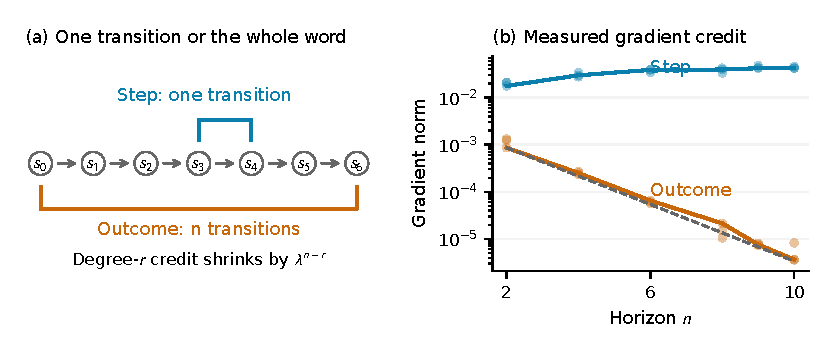
\includegraphics[width=\linewidth]{figures/credit_locality.pdf}
\caption{\textbf{The answer touches $n$ transitions, a step target only one.} (a)~A degree-$r$
feature of the answer is damped by $\mixrate^{n-r}$, and a step target shortens the horizon to $1$.
(b)~Measured on a two-block Transformer at initialization, the answer gradient decays at the
predicted rate $\mixrate=0.5$ per letter and the step gradient does not
(\cref{tab:spectrum}).}
\label{fig:credit}
\end{figure}

\paragraph{Results.} Let $n$ be the horizon, $\initscale$ the initialization scale, and
$\mixrate<1$ the contraction per unseen move. We answer three questions.
\begin{itemize}[leftmargin=*,itemsep=3pt,topsep=3pt]
\item \textbf{Does a solution exist? Yes: exact two-block executors for both formats (\cref{prop:represent}).}
\item \textbf{How does training start? With a credit gap (\cref{thm:main,thm:separation}).}
Outcome interaction credit is at most $C\initscale^6\mixrate^{n-3}$. For counting with a fixed query,
step rule credit is of order $\initscale^6/n$ with high probability, with no factor $\mixrate^n$.
\item \textbf{Is a solution reached? Not by outcome training (\cref{thm:outcome-end}); by step
training once its loss is small (\cref{thm:basin}).} From a zero readout, outcome training stays near
chance and reaches no exact solution for time $\Omega(\mixrate^{-n})$. Step training whose loss falls
below $\pimin/4$ converges to an exact solution, and greedy decoding is then exact (\cref{cor:exact}).
\end{itemize}
Whether step training from initialization reaches that loss remains open. Experiments test whether
joint training does, and test the credit mechanism in deeper and pretrained models.

\paragraph{Scope.} The credit theorems use two blocks, fixed widths, small initialization,
full-batch gradient descent and a fixed ReLU pattern, without LayerNorm.
Target contraction applies to permutation tasks, including non-commuting moves.
A strong horizon penalty requires $\mixrate$ bounded away from $1$.
The counting executors use widths that grow with $n$, separately from the fixed-width training bounds.

Weak gradients for composed targets are known \citep{shalevshwartz2017failures}.
Our contribution is to resolve credit by interaction degree for both a fixed target and
the Transformer Jacobian. This identifies the signal that disappears and the features
that could receive it.

\begin{table}[t]
\centering\small
\begin{tabular*}{\linewidth}{@{\extracolsep{\fill}}lll@{}}
\toprule
Format & Row ($K=3$, start $1$, query \texttt a, word \texttt{banana}) & Loss on\\
\midrule
Outcome & \texttt{1 a b a n a n a SEP : 1 EOS} & ${:}\ \ 1\ \ \textsc{eos}$\\
Step & \texttt{1 a b a n a n a SEP 1 2 2 0 0 1 : 1 EOS} & \texttt{1 2 2 0 0 1} ${:}\ \ 1\ \ \textsc{eos}$\\
\bottomrule
\end{tabular*}
\caption{\textbf{The running example.} Count the letter \texttt a in \texttt{banana} modulo $3$,
starting from $1$. Both formats receive the same prompt; step supervision also generates the
running values.}
\label{tab:rows}
\end{table}

\section{Setup}
\label{sec:setting}

\begin{definition}[State-tracking task]
\label{def:task}
A task has $K$ states, a start state $s_0$, a query $q$ and moves $x_1,\ldots,x_n$, which determine
\begin{equation}
 s_t=F(s_{t-1},x_t),\qquad t=1,\ldots,n.
 \label{eq:tracking}
\end{equation}
The answer is $y=s_n$. Given $q$, the moves are i.i.d.\ and independent of $s_0$. The task is a
\emph{permutation task} if every move $x$ permutes the states; $\bm T_x$ is its permutation matrix,
so $\bm e_{s_t}^\top=\bm e_{s_{t-1}}^\top\bm T_{x_t}$.
\end{definition}
For counting, $x_t=\mathbf 1[w_t=q]$ for the $t$-th letter $w_t$, and $F(s,x)=s+x\bmod K$.

\begin{definition}[Contraction coefficient]
\label{def:lambda}
For a permutation task, let $\overline{\bm T}=\E_x\bm T_x$ and
$\mixrate=\max_q\max_{\bm v\perp\one,\|\bm v\|=1}\|\bm v^\top\overline{\bm T}\|$.
\end{definition}
Always $\mixrate\le1$: one unseen move shrinks the centred state by at most a factor $\mixrate$.
For counting over four uniform letters, $\mixrate=0.5$ at $K=2$ and $0.66$ at $K=3$
(\cref{tab:family} gives the other tasks).

\begin{definition}[Outcome and step losses]
\label{def:losses}
Let $\bm z_t(\theta)\in\R^K$ be the state logits at the position that predicts $s_t$, and $\bm z_\theta$
those at the answer position. The \emph{outcome loss} is $\Lout(\theta)=\E[-\log\softmax(\bm z_\theta)_y]$.
The \emph{step loss} is the teacher-forced loss
$\Lstep(\theta)=\frac1n\sum_{t=1}^n\E[-\log\softmax(\bm z_t(\theta))_{s_t}]$; $\Lstep^{\ge2}$ averages
over $t=2,\ldots,n$ only.
\end{definition}

Fix the start state and the query, so the moves are independent. Every square-integrable function
$f$ of the moves has a unique Efron--Stein decomposition $f=\sum_{S\subseteq[n]}f_S$, where $f_S$
depends only on $x_S$ and has mean zero in each $x_t$, $t\in S$ \citep{efron1981jackknife}.

\begin{definition}[Degree]
\label{def:degree}
The component $f_S$ has \emph{degree} $|S|$, and $(f)_r=\sum_{|S|=r}f_S$. Vector- and
matrix-valued functions are decomposed entrywise.
\end{definition}
For centred moves, $x_1+x_2$ has degree $1$ and $x_1x_2$ has degree $2$. Degree counts input
moves, not powers of parameters.

\begin{assumption}[Architecture]
\label{ass:arch}
A causal Transformer with two blocks of softmax heads and ReLU MLPs, learned token and position
embeddings, no LayerNorm, fixed widths and a linear readout $V$; every logit vector is $\bm z=Vh$ with
$h$ independent of $V$.
\end{assumption}

\begin{assumption}[Initialization]
\label{ass:init}
$\theta_0=\initscale\tilde\theta$, where $\tilde\theta$ has MLP biases $|\tilde b_m|\ge1$ and value-token
embeddings with smallest singular value $\varsigma>0$. We work on
$\initball=\{\theta:\|\theta-\theta_0\|\le\ballradius\initscale\}$ with $\ballradius=\min(1/8,\varsigma/4)$.
\end{assumption}

\begin{assumption}[Task]
\label{ass:task}
The task is a permutation task with contraction $\mixrate<1$.
\end{assumption}

\begin{assumption}[Training]
\label{ass:gd}
Full-batch gradient descent $\theta_{j+1}=\theta_j-\stepsize\nabla L(\theta_j)$ on $\Lout$ or $\Lstep$.
\end{assumption}

On $\initball$, for $\initscale$ below a constant, no ReLU unit changes sign on any input
(\cref{app:network}). Constants $c,C>0$ depend only on the widths, $K$ and $\tilde\theta$, never on
$n$, $\initscale$ or $\stepsize$ (details in \cref{app:assumptions}).

\paragraph{Target spectrum.} On a permutation task, every unseen move contracts the centred state. For every set $S$,
\begin{equation}
 \mathbb E\bigl\|(y-\bm u)_S\bigr\|^2\le\Bigl(1-\frac1K\Bigr)\mixrate^{2(n-|S|)},
 \label{eq:horizon}
\end{equation}
A component on $r$ moves averages over the other $n-r$ moves.
Each unseen move contributes one factor $\mixrate$.
Counting attains the exponent (\cref{rem:tight}).
For $\mixrate$ close to $1$, the bound can be weak at short horizons.
We also measure the target spectrum directly.


\section{Both solutions exist}
\label{sec:executors}

For counting, the same architecture can solve both formats.

\begin{proposition}[Both solutions exist]
\label{prop:represent}
For every $K$, alphabet size and $n$, there is one architecture as in \cref{ass:arch}, with widths
growing linearly in $n$, and parameters $\thstep$ and $\thout$ at which greedy
decoding produces the correct step continuation and the correct outcome continuation, respectively,
on every counting prompt. Both have a positive logit margin on every supervised position and are
exact on an open neighbourhood.
\end{proposition}

\paragraph{Construction.} Block~1 copies the query to each letter and computes its match bit
$b_t=\mathbf 1[w_t=q]$. In the step executor, Block~2 reads $s_{t-1}$ and $b_t$, then looks up
$(s_{t-1}+b_t)\bmod K$. In the outcome executor, it averages the bits, rescales by $n$, and
looks up $(s_0+\sum_t b_t)\bmod K$ (\cref{fig:executors}).
Unused heads and MLP units are zero, so both use the same architecture.
Finite routing scores keep attention leakage below the readout margin.
The positive margin and continuity give the open neighbourhood at each fixed $n$.
\Cref{app:architectures} gives the parameters and proof.
This follows the approach of explicit Transformer constructions
\citep{akyurek2023icl,ramesh2023capable}.

\begin{figure}[t]
\centering
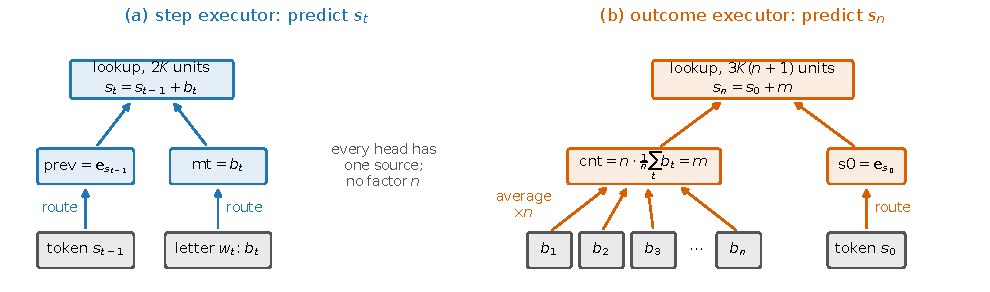
\includegraphics[width=\linewidth]{figures/executors.pdf}
\caption{\textbf{The two executors differ only in their second block.} (a)~The step executor
routes the displayed state and the current bit to a lookup with $2K$ units. (b)~The outcome
executor averages all $n$ bits, multiplies the average by $n$, and looks up $(s_0,m)$ with
$3K(n+1)$ units.}
\label{fig:executors}
\end{figure}


\section{How training starts: a credit gap}
\label{sec:gap}

\paragraph{Model spectrum at initialization.}
At small initialization, attention is nearly uniform and the MLPs are affine on $\initball$.
Uniform attention makes the network additive across positions, with degree at most $1$.
A term with $k\ge1$ attention scores reaches at most $2k+1$ input moves and has Jacobian of size
$C\initscale^2(\attconst\initscale^4)^k$: the first score permits interactions at cost $\initscale^6$, and each
further score costs $\initscale^4$ (\cref{prop:score-degree}).

\subsection{Credit matches degree}
\label{sec:credit}

\begin{definition}[Credit]
\label{def:credit}
For a target signal $g$, a random vector in $\R^K$, let $\cred_g(\theta)=\E\langle\bm z_\theta,g\rangle$.
The \emph{credit} for $g$ is $\|\nabla_\theta\cred_g(\theta)\|$, and the \emph{credit at degrees} $R$ is
$\bigl\|\sum_{r\in R}\E[(\Jz)_r^\top(g)_r]\bigr\|$.
\end{definition}
For the outcome signal $g_{\mathrm{out}}=y-\bm u$, credit is the target-dependent part of the gradient of
$\Lout$ \citep{shalevshwartz2017failures,abbe2025parities}; write $\outcredit=\cred_{g_{\mathrm{out}}}$.
The \emph{interaction credit} is the credit at degrees $r\ge2$.

Represent the answer $y$ as a one-hot vector.
Let $\bm z_\theta$ be the logits, $\hat y=\softmax(\bm z_\theta)$ and $\bm u=\one/K$.
For one prompt, $-\pd{\ell}{\theta}=(\Jz)^\top(y-\hat y)$.
Interactions on different sets of moves are orthogonal.
At uniform prediction, this gives

\begin{equation}
 -\dpd{\Lout}{\theta}
 =\sum_{r=0}^n
 \mathbb E\biggl[
 \Bigl(\dpd{\bm z_\theta}{\theta}\Bigr)_r^{\!\top}
 (y-\bm u)_r
 \biggr].
 \label{eq:grad-split}
\end{equation}
Only matching degrees contribute.
Away from uniform prediction, the same identity holds for the answer-dependent gradient
(\cref{lem:gradient-split}). Define the target and Jacobian spectra by

\begin{equation}
 A_r:=\mathbb E\bigl\|(y-\bm u)_r\bigr\|^2,
 \qquad
 J_r(\theta):=\mathbb E\bigl\|(\Jz)_r\bigr\|_F^2.
 \label{eq:spectra}
\end{equation}
Cauchy--Schwarz gives
\[
 \boxed{\text{degree-$r$ credit}\le\sqrt{A_rJ_r}}.
\]
Credit is small wherever either spectrum has little mass.

\subsection{Why outcome optimization stalls}
\label{sec:spectrum}

\begin{figure}[t]
\centering
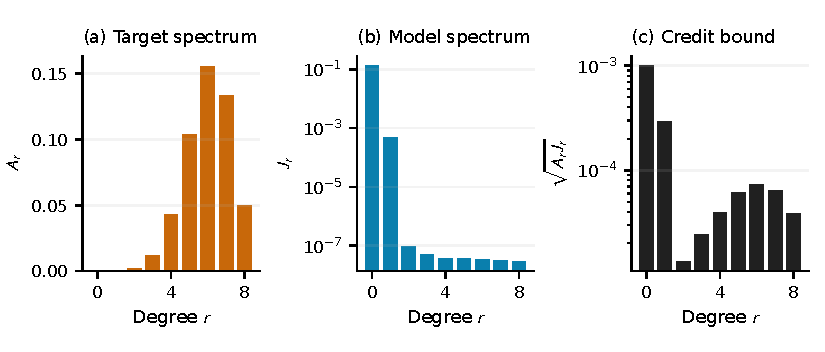
\includegraphics[width=\linewidth]{figures/overlap_spectra.pdf}
\caption{\textbf{The answer and a fresh network barely overlap.} Counting, $K=2$, $n=8$.
(a)~The target spectrum $A_r$ puts its mass at high degree. (b)~The Jacobian spectrum $J_r$ of the
two-block Transformer at initialization is $99.6\%$ degree~$0$. (c)~The bound $\sqrt{A_rJ_r}$ on the
degree-$r$ credit.}
\label{fig:overlap}
\end{figure}

\paragraph{Outcome credit and the plateau.}
\label{sec:main}

\begin{theorem}[Outcome interaction credit]
\label{thm:main}
Suppose \cref{ass:arch,ass:init,ass:task} hold, and fix the start state and the query. For all
$n\ge2$, all $\initscale$ with $\initscale^2\le c\mixrate$, and all $\theta\in\initball$, the interaction credit for
$y-\bm u$ is at most $C\initscale^6\mixrate^{n-3}$.
\end{theorem}

Each attention score costs $\initscale^4$ and reaches at most two more moves, while each unseen move costs
$\mixrate$; summing over scores gives the bound (\cref{eq:score-credit,lem:score-sum}). It holds along every unit direction, including
toward an exact executor. With a nonzero readout, the full gradient is at most
$C\initscale(\initscale^2+\mixrate^n)$, so training stays in $\initball$ for time $\Omega(\min(\initscale^{-2},\mixrate^{-n}))$
(\cref{prop:plateau}); a zero readout removes the cap (\cref{thm:outcome-end}), and from a zero readout the
measured exit time grows at least as fast as $\mixrate^{-n}$ (\cref{fig:regime}).

\subsection{Why step optimization is different}
\label{sec:steps}

Teacher forcing supplies the previous state.
The next target has a one-move horizon.
Its gradient can still learn only the average move rather than the rule.
We separate these two signals:

\[
 \bm e_{s_t}-\bm u
 =\underbrace{\overline{\bm T}^\top\bm e_{s_{t-1}}-\bm u}_{\text{prior}}
 +\underbrace{\bm e_{s_t}-\overline{\bm T}^\top\bm e_{s_{t-1}}}_{\text{rule}}.
\]
The \emph{rule signal} $g_{{\mathrm{rule}},t}=\bm e_{s_t}-\overline{\bm T}^\top\bm e_{s_{t-1}}$ is the part of the
next state not predicted by the previous one. Let $\rulecredit=\E_t\E\langle\bm z_t,g_{{\mathrm{rule}},t}\rangle$,
with $t$ uniform on $\{2,\ldots,n\}$; $\|\nabla\rulecredit\|$ is the credit of \cref{def:credit} with
the local rule as signal.

\begin{theorem}[Step credit]
\label{thm:separation}
Suppose \cref{ass:arch,ass:init,ass:task} hold and the start state is uniform.
\begin{enumerate}[label=(\roman*),leftmargin=*,itemsep=0pt,topsep=2pt]
\item For all $n\ge2$, $\initscale\le c\mixrate$ and $\theta\in\initball$,
$\|\nabla \Lstep^{\ge2}(\theta)\|\ge c\,\initscale\mixrate$ and $\|\nabla \Lout(\theta)\|\le C\initscale(\initscale^2+\mixrate^n)$.
\item For all $n\ge2$, $\initscale\le c$ and $\theta\in\initball$, $\|\nabla\rulecredit(\theta)\|\le C\initscale^6/n$.
\item Consider counting with a fixed query of match probability $p<1/2$, fixed MLP biases as in
\cref{ass:init}, and all other entries of $\tilde\theta$ i.i.d.\ uniform on $[-1,1]$. For every
$\failprob\in(0,1)$ there exist $a_\failprob,\initscale_\failprob>0$ such that for every $n\ge2$, with probability at
least $1-\failprob$ over $\tilde\theta$, $\|\nabla\rulecredit(\initscale\tilde\theta)\|\ge a_\failprob\initscale^6/n$ for all $\initscale\in(0,\initscale_\failprob]$.
\end{enumerate}
\end{theorem}

Part (i) comes from the displayed state and teaches the average move.
The rule also needs the current letter.
It pays $\initscale^6$ for a score correction and $1/n$ to select that letter, but no
exponential horizon factor.

For each fixed $n$ and sufficiently small $\initscale$, step rule credit exceeds the outcome
interaction bound by at least order $\mixrate^{-(n-3)}/n$ with high probability.
This comparison excludes the prior and degrees $0$--$1$ (\cref{tab:matched}).
At $\initscale=0.02$, the measured ratio under a uniform start grows from $64$--$119$ at $n=4$
to $9{,}410$--$21{,}300$ at $n=14$.
The theorem does not certify this scale.

\section{Which solution is reached}
\label{sec:end}
\label{sec:lookup}

Both executors of \cref{prop:represent}, with rescaled readouts, lie in the open basin of their own
loss (\cref{lem:end-nonempty}).
The formats differ in whether training reaches one.

\begin{definition}[Supervised loss and basin]
\label{def:basin}
A \emph{supervised loss} is $L(\theta)=\sum_{i\in\items}\pi_i\ell_i(\theta)$ over a finite set $\items$ of
items, each a prompt with a supervised position, where $\pi_i>0$, $\sum_i\pi_i=1$ and $\ell_i$ is the
cross-entropy of the gold token. Let $\pimin=\min_i\pi_i$. The \emph{basin} of $L$ is
$\basin(L)=\{\theta:L(\theta)<\pimin/4\}$.
\end{definition}
For $\Lstep$ the items are the pairs $(\omega,t)$ of a prompt and a state position, with
$\pi_{(\omega,t)}=\pi_\omega/n$, where $\pi_\omega$ is the probability of prompt $\omega$; for $\Lout$ there is one item per prompt.

\begin{theorem}[Outcome training does not converge]
\label{thm:outcome-end}
Suppose \cref{ass:arch,ass:init,ass:task,ass:gd} hold and the readout of $\tilde\theta$ is zero. There is
$\stepsize_0>0$ such that for all $n\ge2$, $\initscale\le c\mixrate$, $\stepsize\le\stepsize_0$ and $j\le c\mixrate^{-n}/\stepsize$, gradient
descent on $\Lout$ satisfies $\theta_j\in\initball$ and
\[
 \Lout(\theta_j)\ge\log K-C\initscale^2\mixrate^n,
 \qquad
 \E\softmax(\bm z_{\theta_j})_y\le\frac1K+C\initscale\mixrate^{n/2}.
\]
\end{theorem}

The time bound does not depend on $\initscale$; measured times at $\initscale=0.02$ and $0.002$ coincide by $n=14$
(\cref{app:exp-regime}). The same bound holds for gradient flow (\cref{rem:flow}). For $\initscale$ below a constant, $\Lout(\theta_j)\ge\log2-\frac14>\pimin/4$,
so $\theta_j\notin\basin(\Lout)$. A zero readout leaves \cref{thm:separation}
unchanged (\cref{rem:zero-readout}); for $\mixrate=0$ the time is of order $\initscale^{-(2n-1)}$ (\cref{rem:end-parity}).

\begin{assumption}[Backtracking step sizes]
\label{ass:armijo}
From $\theta_j$, the step size is $\stepsize_j=\bar\stepsize\,b^{u_{\mathrm{bt}}}$ for the smallest
$u_{\mathrm{bt}}\ge0$ such that
\begin{equation}
 L(\theta_j-\stepsize_j\nabla L(\theta_j))\le L(\theta_j)-\tfrac{\stepsize_j}2\|\nabla L(\theta_j)\|^2,
 \tag{Armijo}\label{eq:descent}
\end{equation}
with fixed $\bar\stepsize>0$ and $b\in(0,1)$, and $L$ is continuously differentiable near each iterate.
\end{assumption}
This is the Armijo rule \citep{nocedal2006numerical}; with finitely many prompts, $L$ is smooth wherever
no ReLU pre-activation is exactly zero.

\begin{theorem}[Step training converges in the basin]
\label{thm:basin}
Let $L$ be a supervised loss with logits as in \cref{ass:arch}, and let $\theta_{j+1}=\theta_j-\stepsize_j\nabla L(\theta_j)$
with step sizes as in \cref{ass:armijo} for $j\ge \entryidx$. Suppose $\theta_{\entryidx}\in\basin(L)$, and let $L_{\entryidx}=L(\theta_{\entryidx})$,
$\margin_{\entryidx}=\log(\pimin/(2L_{\entryidx}))$ and $\traintime_j=\sum_{i=\entryidx}^{j-1}\stepsize_i$. Then for every $j\ge \entryidx$:
\begin{enumerate}[label=(\roman*),leftmargin=*,itemsep=0pt,topsep=2pt]
\item $\theta_j\in\basin(L)$, and on every item the gold token has the strictly largest logit;
\item $L(\theta_j)\le L_{\entryidx}\big/\bigl(1+\frac{\margin_{\entryidx}^2}{32}\log(1+2L_{\entryidx}\traintime_j/\|V_{\entryidx}\|_F^2)\bigr)$.
\end{enumerate}
\end{theorem}
The rate in (ii) is a worst case that assumes nothing about how the features move.

\begin{corollary}[Exact generation]
\label{cor:exact}
Let $\Lstep^{\mathrm{full}}$ supervise every generated token of the step format: the states, the
formatting tokens and the final answer. Under the hypotheses of \cref{thm:basin} for
$\Lstep^{\mathrm{full}}$, greedy decoding generates the exact step continuation on every supported
prompt at every update $j\ge \entryidx$. If moreover $\traintime_j\to\infty$, then $L(\theta_j)\to0$.
\end{corollary}

\paragraph{Certifying the middle.}
We do not prove that step training from $\theta_0$ enters $\basin(\Lstep)$. Instead, in a full-batch run
that verifies \cref{eq:descent}, the first update $\entryidx$ with $\Lstep(\theta_{\entryidx})<\pimin/4$ certifies
convergence to an exact solution (\cref{thm:basin}).

\begin{table}[t]
\centering\small
\fitwidth{\begin{tabular}{@{}lcccc@{}}
\toprule
part of the gradient at $\theta_0$ & bound scale & $n=4$ & $n=8$ & $n=12$\\
\midrule
\multicolumn{5}{@{}l}{\emph{Absorbed by single-position features}}\\
step: prior & $\initscale\mixrate$ & $3.3\mathrm{e}{-2}$ & $3.3\mathrm{e}{-2}$ & $3.3\mathrm{e}{-2}$\\
outcome: degrees $0$ and $1$ & $\initscale\mixrate^n$ & $1.6\mathrm{e}{-4}$ & $6.7\mathrm{e}{-6}$ & $3.2\mathrm{e}{-7}$\\
\midrule
\multicolumn{5}{@{}l}{\emph{Requires interactions}}\\
step: rule credit $\|\nabla\rulecredit\|$ & $\initscale^6/n$ & $3.3\mathrm{e}{-9}$ & $1.8\mathrm{e}{-9}$ & $1.1\mathrm{e}{-9}$\\
outcome: degrees $\ge2$, start state fixed & $\initscale^6\mixrate^{n-3}$ & $1.4\mathrm{e}{-9}$ & $1.9\mathrm{e}{-10}$ & $1.6\mathrm{e}{-11}$\\
outcome: degrees $\ge2$, uniform start & $\initscale^6\mixrate^{n-3}$ & $2.8\mathrm{e}{-11}$ & $2.6\mathrm{e}{-12}$ & $1.7\mathrm{e}{-13}$\\
\bottomrule
\end{tabular}}
\caption{\textbf{Rule credit has polynomial horizon cost; outcome interaction credit has exponential cost.} Norm of each
part of the gradient at initialization, with the scale of its theorem bound. Counting, $K=2$, $\mixrate=\frac12$,
$\initscale=0.02$, exact over all words (\cref{app:exp-regime}).}
\label{tab:matched}
\end{table}

\begin{figure}[t]
\centering
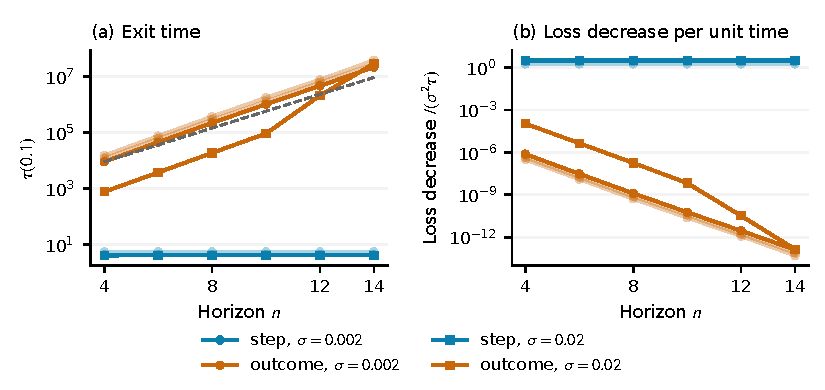
\includegraphics[width=\linewidth]{figures/regime_both.pdf}
\caption{\textbf{Outcome exit time grows at least as fast as $\mixrate^{-n}$; step exit time stays constant.}
Runs satisfy the assumptions of \cref{thm:outcome-end}, with a zero initial readout. Counting, $K=2$, $\mixrate=0.5$,
$\initscale=0.002$ and $0.02$, exact full-batch loss, no ReLU unit switching. (a)~Training time to leave the ball.
(b)~Loss decrease per unit time, in units of $\initscale^2$. Faint lines: two more draws of $\tilde\theta$.}
\label{fig:regime}
\end{figure}

\newpage
\section{Experiments test the mechanism}
\label{sec:validation}

We first test the bounds inside their assumptions (\cref{app:exp-regime}).
We then test the mechanism with LayerNorm, deeper models and LoRA.
Besides counting, we use Boolean-8 and a reversible register machine.
\Cref{tab:main} summarizes held-out accuracy; \cref{app:experiments} gives the protocols.

\begin{table}[t]
\centering\small
\fitwidth{\begin{tabular}{@{}llccccc@{}}
\toprule
Task & Model & $n$ & $\mixrate$ & outcome & step & chance\\
\midrule
count mod $2$ & two-block & $16$ & $0.50$ & $49$--$52$ & $100$ ($9$ of $10$ seeds) & $50$\\
count mod $3$ & two-block & $16$ & $0.66$ & $30$--$50$ & $100$ & $33$\\
first occurrence (control) & two-block & $8$--$24$ & -- & $71$--$100$ & $80$--$99$ & --\\
Boolean-8 & GPT-2L & $8$ & $0.82$ & $7.7$ & $82$ & $6.25$\\
register machine & GPT-2L & $16$ & $0.95$ & $6.3$ & $99.9$ & $5.9$\\
Boolean-8 & Qwen2.5-0.5B LoRA & $8$ & $0.82$ & $11.1$ & $98.3$ & $6.25$\\
\midrule
BBH, $3$ objects & Qwen2.5-0.5B LoRA & $3$ & $0$ & $35.2$ & $98.4$--$100$ & $33$\\
BBH, $5$ objects & Qwen2.5-0.5B LoRA & $5$ & $0.50$ & $80.0$--$94.4$ & $46$--$100$ & $20$\\
BBH, $7$ objects & Qwen2.5-0.5B LoRA & $7$ & $0.67$ & $15.2$--$24.4$ & $96.4$--$100$ & $14$\\
\bottomrule
\end{tabular}}
\caption{\textbf{Answers alone fail where the answer has no low-degree part; steps succeed.}
Accuracy (\%) on held-out prompts, ranges over seeds; the BIG-Bench Hard rows test on the $750$ real
items. First occurrence keeps a degree-$1$ part at every $n$, and outcome learns it. For count mod $2$ at $n=16$,
step accuracy is after $16$k updates and outcome after $32$k, twice the step budget. Protocols and per-seed results are
in \cref{app:experiments}.}
\label{tab:main}
\end{table}

\subsection{Spectra and gradients at initialization}

\paragraph{Predictions 1 and 2: degree mismatch.}
At initialization, the two-block Transformer's Jacobian puts $99.6\%$ of its mass at
degree $0$ (\cref{fig:overlap}). The targets put most of their mass at high degree.
For Boolean-8 and the register machine, $98.9\%$ and $99.9\%$ of answer variance is at
degrees $\ge2$.
The pattern also appears in Qwen2.5-0.5B.
On three-object BIG-Bench Hard, only $0.022\%$ of the LoRA Jacobian energy is at degree $3$,
the answer's only degree (\cref{app:exp-spectra}).

\paragraph{Prediction 3: gradient decay.}
Exact sums over counting prompts give answer-dependent gradient decay of $0.48$--$0.51$
per letter, close to $\mixrate=0.5$.
The step gradient grows $2.4$-fold from $n=2$ to $10$
(\cref{fig:credit,tab:spectrum}).

\subsection{Training}

\begin{samepage}
\paragraph{Prediction 4: plateau and escape.}
Across $120$ counting runs at $n=6$--$16$, outcome training solves none and step training
solves $60$ (\cref{app:exp-plateau}).
Step learning is still slow and seed-dependent: rule credit starts at order $\initscale^6$.
At $\initscale=0.1$, every tested step seed solves, while outcome training stays at chance
at $n=16$.
During the outcome plateau, at most $2\times10^{-6}$ of the Jacobian energy lies above
degree $1$ in the run shown in \cref{tab:main-evidence}.
\par
\end{samepage}

\begin{table}[!b]
\centering\small
\begin{tabular}{@{}lcc@{}}
\toprule
outcome updates & share above degree $1$ & accuracy\\
\midrule
initialization & $2.4\mathrm{e}{-6}$ & --\\
$1{,}000$ & $1.1\mathrm{e}{-8}$ & $52\%$\\
$3{,}000$ & $1.1\mathrm{e}{-8}$ & $48\%$\\
$6{,}000$ & $2.0\mathrm{e}{-6}$ & $48\%$\\
$8{,}000$ (escaping) & $0.155$ & $55\%$\\
\bottomrule
\end{tabular}
\caption{\textbf{The outcome plateau stays low-degree.} Counting, $K=2$, $n=8$: share of the
outcome model's Jacobian energy above degree $1$ during training, and answer accuracy.}
\label{tab:main-evidence}
\end{table}

\subsection{Transfer to a pretrained model}

\paragraph{Prediction 5: real object tracking.}
We train rank-8 LoRA on generated BIG-Bench Hard tracking\_shuffled\_objects items
\citep{suzgun2022challenging}. We test on all $750$ real benchmark items.
At three objects, $\mixrate=0$ and the answer is pure top degree.
Outcome training stays at the majority-option rate; step training reaches $98$--$100\%$.
The five- and seven-object results are less uniform (\cref{tab:main}).
\Cref{sec:discussion} discusses what the low-degree signal can predict.

\section{Related work}
\label{sec:related}

\paragraph{Intermediate supervision.}
Scratchpads and process supervision
\citep{nye2021scratchpads,uesato2022solving,wei2022cot,lightman2023verify}
have been studied through task decomposition \citep{wies2023subtask}, locality
\citep{prystawski2023think,abbe2024globality} and expressivity
\citep{feng2023towards,merrill2024expressive}.
Outcome supervision need not be statistically harder \citep{jia2025verify}.
Chain supervision can have better sample complexity
\citep{hanneke2026samplecomplexityautoregressivereasoning}.
We study how a fixed network distributes gradient credit at initialization.

\paragraph{Composed targets and gradient signal.}
\citet{shalevshwartz2017failures} show exponentially weak target-dependent gradients
across families of composed targets.
We decompose the credit of one fixed target and a concrete Transformer by degree.
Staircase and leap analyses
\citep{abbe2021staircase,abbe2022mergedstaircase,abbe2023sgd}
study when SGD can learn high-degree targets.
For our counting targets at $\mixrate>0$, all degrees are present.
Their size, rather than their absence, limits credit.
Step targets are known to help with parity and group tracking
\citep{wen2024sparse,liu2023automata}. \citet{panigrahi2025progressive} show that intermediate teacher
checkpoints supply low-degree signal that the final teacher lacks, reducing the sample complexity of
sparse parity; intermediate states play the same role here, and we analyze optimization rather than
sample complexity.

\paragraph{Hardness for a single target.}
\citet{abbe2025parities} prove that noisy gradient descent on a two-layer network stays at
chance on high-degree parities for $\exp(o(d))$ steps under Gaussian initialization, while
Rademacher initialization learns them; their argument is limited to the correlation loss.
\Cref{thm:outcome-end} concerns one fixed target for a Transformer under cross-entropy and exact
gradient descent. Its time $\mixrate^{-n}$ comes from the contraction of the target, resolved degree by degree.

\paragraph{Chain of thought for parity.}
\citet{kim2024parity} prove that a one-layer Transformer with position-only attention and a fixed
nonlinearity learns $k$-parity in one teacher-forced gradient step, and that gradient methods
without intermediate supervision fail for a parity drawn at random from a class. Their signal is
the degree-$2$ local interaction that our rule credit measures. Our negative result concerns one
fixed target; our positive result holds once the loss falls below an explicit threshold, for a
Transformer that learns its computation.

\paragraph{Permutation learning.}
\citet{wang2025compositional} study compositions of hidden permutations.
They give a statistical-query lower bound and a curriculum result at depth $O(\log k)$
\citep{sanford2024transformers}.
Our target is fixed, and displayed states permit constant-depth executors.
Their convergence result uses simplified dynamics; ours is local (\cref{thm:basin}).
\citet{li2025noise} decompose the target using Efron--Stein; we also decompose the Jacobian.
In single-layer Transformers on Markov data, the unigram solution can be stationary
\citep{makkuva2025attention,makkuva2024local}.
Here, outcome credit is small but need not vanish.

\section{Discussion}
\label{sec:discussion}

\paragraph{When do steps help?}
Low-degree answer variance estimates how much signal a fresh network can use; it is a diagnostic.
Five-object BIG-Bench Hard has only $1.56\%$ at degrees $0$--$1$, yet outcome training learns.
Its degree-$1$ signal is damped by $\mixrate^4=1/16$, rather than removed.
Low-degree share orders learning in the fixed-swap pilots, but not across swap counts (\cref{tab:bbh-pilot}).

\paragraph{Initialization scale.}
The target spectrum does not depend on initialization; the Jacobian spectrum does.
Larger initialization can improve step training, as the measured runs show.
The small-initialization bounds do not rule out outcome learning at other scales.

\paragraph{Parity.}
Counting modulo $2$ with match probability $1/2$ has $\mixrate=0$: only degree $n$ remains, giving
leap $n$ \citep{abbe2023sgd}. \Cref{rem:lambda-zero} handles this case.

\paragraph{Limitations.}
The assumptions in \cref{sec:intro} restrict the credit theorems.
AdamW runs allow ReLU switching and test the mechanism outside that regime
(\cref{rem:two-block-bias}).
The missing training result is entry into the step basin.
We have not tested large-scale training.

\paragraph{Conclusion.}
Interaction degree links the target to the gradient features available for learning,
explaining weak outcome credit and the signal retained by step targets.
Proving that step training reaches the basin is the remaining step.
            % abstract through conclusion

%%%%%%%%%%%%%%%%%%%%%%%%%%%%%%%%%%%%%%%%%%%
%%% Bibliography
\clearpage
\bibliographystyle{plainnat}
\bibliography{main}

%%%%%%%%%%%%%%%%%%%%%%%%%%%%%%%%%%%%%%%%%%%%%%%%%%%%%%%%
% APPENDIX (appendix.tex): notation; A model and constructions; B proofs for
% permutation tasks; C the transition model; D proofs for wrong traces;
% E experimental details; F reproducibility.
%%%%%%%%%%%%%%%%%%%%%%%%%%%%%%%%%%%%%%%%%%%%%%%%%%%%%%%%

\clearpage
\appendix
\counterwithin{theorem}{section}
\counterwithin{lemma}{section}
\counterwithin{proposition}{section}
\counterwithin{corollary}{section}
\counterwithin{definition}{section}
\counterwithin{remark}{section}
\raggedbottom
\setlength{\parskip}{2pt plus 1pt minus 1pt}
\setlength{\abovedisplayskip}{8pt plus 2pt minus 2pt}
\setlength{\belowdisplayskip}{8pt plus 2pt minus 2pt}
\setlist[itemize]{itemsep=2pt,topsep=3pt}
\setlist[enumerate]{itemsep=2pt,topsep=3pt}

% !TEX root = main.tex
% Appendix. A: executors. B: theorem arguments followed by technical verification.
% C: numerical verification of the theory. D: experiments by prediction. E: reproducibility.
\providecommand{\Zk}{\mathbb Z_K}
\providecommand{\reg}[1]{\ensuremath{\mathsf{#1}}}
\providecommand{\op}[1]{\textsc{#1}}

\section*{Roadmap}
\addcontentsline{toc}{section}{Roadmap}

The table maps results to assumptions, proofs and numerical checks.
\Cref{app:experiments} gives the training protocols and results.
\Cref{app:reproducibility} lists the code and compute.

\begin{center}\small
\fitwidth{\begin{tabular}{@{}llll@{}}
\toprule
Result & Assumptions & Proof & Numerical check\\
\midrule
\Cref{eq:grad-split}: credit matches degree & independent moves & \cref{app:tools} & exact gradients, \cref{app:exp-spectra}\\
\Cref{eq:horizon}: every unseen move costs $\mixrate$ & (A3) & \cref{lem:target-contraction} & \cref{tab:verify}, row 1\\
\Cref{prop:represent}: both executors in two blocks & (A1) & \cref{app:exact} & \cref{tab:verify}, row 8\\
\Cref{thm:main}: outcome interaction credit & (A1)--(A3), $0<\mixrate<1$ & \cref{app:thm1} & \cref{tab:verify}, rows 2--3\\
\Cref{prop:plateau}: plateau with a nonzero readout & (A1)--(A4), $0<\mixrate<1$ & \cref{app:thm1} & \cref{tab:verify}, row 4; \cref{app:exp-regime}\\
\Cref{thm:separation}: horizon-free gradient and rule credit & (A1)--(A3), uniform start & \cref{app:thm2} & \cref{tab:verify}, rows 5--7; \cref{app:exp-regime}\\
\Cref{thm:outcome-end}: outcome never reaches the basin & (A1)--(A3), $\initscale\le c\mixrate$, $\tilde V=0$ & \cref{app:end} & --\\
\Cref{thm:basin}, \cref{cor:exact}: convergence in the basin & Armijo steps, \cref{ass:armijo} & \cref{app:end} & --\\
\bottomrule
\end{tabular}}
\end{center}

%=============================================================================
\section{Exact two-block executors}
\label{app:architectures}

We prove \cref{prop:represent} and list the nonzero parameters.

\subsection{Program overview}

The table specifies the operations in each block.
$\widetilde s_{t-1}$ denotes the displayed previous state.
All state arithmetic is modulo $K$.

\begin{center}\small
\begin{tabular}{@{}llll@{}}
\toprule
Program part & Reads & Writes & Purpose\\
\midrule
Block 1, head & query token & $\reg{qry}$ & copy the query to letter positions\\
Block 1, MLP & letter, $\reg{qry}$ & $\reg{match}$ & compute $b_t$\\
\midrule
Step, block 2, head 1 & previous value & $\reg{prev}$ & copy $\widetilde s_{t-1}$\\
Step, block 2, head 2 & $\reg{match}$ at letter $t$ & $\reg{mt}$ & copy $b_t$\\
Step, block 2, MLP & $\reg{prev}$, $\reg{mt}$ & $\reg{out}$ & compute $s_t$\\
\midrule
Outcome, block 2, head 1 & $\reg{match}$ at all letters & $\reg{cnt}$ & compute $m=\sum_tb_t$\\
Outcome, block 2, head 2 & start value & $\reg{s0}$ & copy $s_0$\\
Outcome, block 2, MLP & $\reg{s0}$, $\reg{cnt}$ & $\reg{out}$ & compute $s_n$\\
\bottomrule
\end{tabular}
\end{center}

A \emph{route} copies a register from one source position.
An \emph{average} reads several sources.
A \emph{lookup} maps an input pair to its output.

\subsection{Architecture, layout and primitives}
\label{app:construction}
\label{app:model}

\textbf{Architecture.} Each block has three heads and one MLP, without LayerNorm.
For this construction, the head dimension $d$ equals the number of positions:

\begin{align*}
 h_i&\leftarrow h_i+\sum_{h=1}^{3}\sum_{j\le i}
 \operatorname{softmax}_{j\le i}\!\Big(\tfrac{1}{\sqrt d}(W^{(h)}_Qh_i)^{\!\top}W^{(h)}_Kh_j\Big)\,W^{(h)}_Vh_j,\\
 h_i&\leftarrow h_i+W_{\mathrm{out}}\relu(W_{\mathrm{in}}h_i+b_{\mathrm{in}}),
 \qquad
 \mathrm{logits}_i=V\,h_i .
\end{align*}

\textbf{Registers.} The residual stream is split into the registers of the table, in this order,
with $d=2n+6$ positions and MLP width $\max\{|\Sigma|,3K(n+1),2n+1\}$:
\[
 \underbrace{\reg{tl}}_{|\Sigma|}\;\underbrace{\reg{tv}}_{K}\;\underbrace{\reg{pos}}_{d}\;
 \underbrace{\reg{qry}}_{|\Sigma|}\;\underbrace{\reg{match}}_{1}\;\underbrace{\reg{prev}}_{K}\;
 \underbrace{\reg{mt}}_{1}\;\underbrace{\reg{cnt}}_{1}\;\underbrace{\reg{s0}}_{K}\;
 \underbrace{\reg{out}}_{K},
 \qquad d_{\mathrm{res}}=2|\Sigma|+4K+d+3 .
\]
$\reg{tl}$ and $\reg{tv}$ hold the token (a letter or a value) and $\reg{pos}$ the position, all
one-hot. $\reg r[a]$ is coordinate $a$ of register $\reg r$, and $E_{\reg a\leftarrow\reg b}$ is the
$d_{\mathrm{res}}\times d_{\mathrm{res}}$ matrix that copies register $\reg b$ into register $\reg a$.

\textbf{Tokens and positions.} Letters are $0,\ldots,|\Sigma|-1$, value $v$ is $|\Sigma|+v$, and SEP,
``:'' and EOS follow. Positions are $0$-indexed:
\begin{align*}
 \text{prompt: }&\ s_0@0,\quad q@1,\quad w_t@(1+t),\quad \text{SEP}@(n+2),\\
 \text{step: }&\ s_t@(n+2+t),\quad \text{``:''}@(2n+3),\quad s_n@(2n+4),\\
 \text{outcome: }&\ \text{``:''}@(n+3),\quad s_n@(n+4).
\end{align*}
Position $i$ predicts the token at $i+1$, so $n+1+t$ predicts $s_t$ in the step row and $n+3$
predicts $s_n$ in the outcome row.

\textbf{Route and average.} Give source positions score $\beta_n$ and all others score $0$.
Let $\mathrm{src}(i)\subseteq\{0,\ldots,i\}$ be the source set.
Unlisted positions use the fallback $\{f\}$.
Set $C_Q=\beta_n\sqrt d$ and $\beta_n=\max\{16,3\log(8(n+3))\}$:

\begin{equation}
 \begin{aligned}
 (W_K)_{j,\reg{pos}[j]}=1,\quad
 (W_Q)_{j,\reg{pos}[i]}&=C_Q\quad(j\in\mathrm{src}(i)),\\
 \tfrac1{\sqrt d}(W_Qh_i)^\top W_Kh_j&=\beta_n\,[j\in\mathrm{src}(i)].
 \end{aligned}
 \label{eq:route}
\end{equation}
With $W_V=E_{\reg a\leftarrow\reg b}$, the head writes the average of register $\reg b$ over $\mathrm{src}(i)$
into $\reg a$, up to a small leak. One source is a route and several are an average. A fallback
$f>i$ gives uniform attention at a position that predicts nothing supervised.

\textbf{Lookup.} Use one unit per input pair.
For one-hot inputs, let $\mathrm{pre}_{s'x'}=[s=s']+[x=x']-3/2$.
Only the matching pair has positive pre-activation, equal to $1/2$.
Output weights $2\bm e_{F(s',x')}$ give

\begin{equation}
 \textstyle\sum_{s',x'}2\,\bm e_{F(s',x')}\relu(\mathrm{pre}_{s'x'})=\bm e_{F(s,x)}.
 \label{eq:lookup}
\end{equation}

\subsection{Both programs are exact}
\label{app:exact}


\begin{proof}[Proof of \cref{prop:represent}]
\proofstep{Ideal routing.}
The parameters in \cref{app:params} give
\begin{align*}
 \reg{match}_{1+t}
 &=2\sum_{a\in\Sigma}\relu([w_t=a]+[q=a]-3/2)=b_t,\\
 \reg{prev}_{n+1+t}&=\bm e_{s_{t-1}},\qquad
 \reg{mt}_{n+1+t}=b_t,\\
 2\relu([s_{t-1}=j]+[b_t=\iota]-3/2)
 &=[(s_{t-1},b_t)=(j,\iota)],\\
 \reg{out}_{n+1+t}
 &=\sum_{j,\iota}\bm e_{j+\iota}[(s_{t-1},b_t)=(j,\iota)]
 =\bm e_{s_t}.
\end{align*}
For the outcome program,
\begin{align*}
 \reg{cnt}_{n+3}&=n\left(\frac1n\sum_{t=1}^nb_t\right)=m,
 \qquad\reg{s0}_{n+3}=\bm e_{s_0},\\
\end{align*}
\[
 \relu(m-a+1)-2\relu(m-a)+\relu(m-a-1)=[m=a].
\]
\begin{align*}
 \reg{out}_{n+3}&=\sum_{j,a}\bm e_{j+a}[s_0=j][m=a]\\
 &=\bm e_{s_0+m}=\bm e_{s_n}.
\end{align*}
All state indices are modulo $K$; the readout in \cref{app:params} supplies formatting and the final answer.

\proofstep{Finite-score error.}
With $d=2n+6$ and $\beta_n=\max\{16,3\log(8(n+3))\}$,
\[
 \rho_n=(d-1)e^{-\beta_n}
 <\frac{2(n+3)}{(8(n+3))^3}
 =\frac1{256(n+3)^2}.
\]
The routing and lookup errors satisfy
\begin{align*}
 |\reg{match}-b_t|&\le2\rho_n,\\
 \|\reg{prev}-\bm e_{s_{t-1}}\|&\le\rho_n,
 \quad |\reg{mt}-b_t|\le3\rho_n,\\
 \mathrm{pre}_{\mathrm{correct}}&\ge\tfrac12-4\rho_n>0>\mathrm{pre}_{\mathrm{other}},
 \quad\reg{out}_{s_t}\ge1-8\rho_n,\\
 |\reg{cnt}-m|&\le3n\rho_n,
 \quad\|\reg{s0}-\bm e_{s_0}\|\le\rho_n,\\
 e_{\mathrm{leak}}&=3n\rho_n+(n+2)\rho_n<\tfrac1{192},\\
 \reg{out}_{s_n}&\ge1-e_{\mathrm{leak}},
 \quad\reg{out}_{\mathrm{other}}\le e_{\mathrm{leak}}.
\end{align*}
The three-ReLU equality test is $1$-Lipschitz. Thus every supervised position has margin
\[
 z_{\mathrm{correct}}-\max_{a\ne\mathrm{correct}}z_a
 \ge\min\{20(1-8\rho_n),20(1-2e_{\mathrm{leak}})\}>19.
\]

\proofstep{Open neighbourhood.}
For fixed $n$, let $\mathcal P_n$ be the finite set of supported gold prefixes and prediction positions.
Continuity and the preceding margin give $\ballradius_{\mathrm{exec},n}>0$ such that
\[
 \|\theta-\theta^\star\|<\ballradius_{\mathrm{exec},n}
 \quad\Longrightarrow\quad
 \max_{P\in\mathcal P_n}\|\bm z_\theta(P)-\bm z_{\theta^\star}(P)\|_\infty<19/2.
\]
Every greedy prediction remains correct. Induction over the continuation proves the claim.
\end{proof}


\subsection{Explicit parameters}
\label{app:params}

All unspecified entries are zero.
The reconstruction script checks these tensors against the implementation entry by entry
(\cref{app:reproducibility}).

\textbf{Embeddings.}
$(W_{\mathrm{te}})_{a,\reg{tl}[a]}=1$, $(W_{\mathrm{te}})_{|\Sigma|+v,\reg{tv}[v]}=1$ and $(W_{\mathrm{pe}})_{i,\reg{pos}[i]}=1$.

\textbf{Block 1 (shared): the match bit.} A route copies the query letter to each letter
position, and a lookup with one unit per letter tests whether the two letters agree:
\begin{align*}
 \text{head 1: }&\ \mathrm{src}(1+t)=\{1\}\ (t=1,\ldots,n),\quad f=0,\quad W_V=E_{\reg{qry}\leftarrow\reg{tl}},\\
 \text{MLP unit }a:&\ (W_{\mathrm{in}})_{a,\reg{tl}[a]}=(W_{\mathrm{in}})_{a,\reg{qry}[a]}=1,\quad
 (b_{\mathrm{in}})_a=-\tfrac32,\quad (W_{\mathrm{out}})_{\reg{match},a}=2,
\end{align*}
so $\reg{match}_{1+t}=2\sum_a\relu([w_t=a]+[q=a]-\frac32)=b_t$. Heads 2 and 3 are zero, and non-letter
positions get $\reg{qry}=\reg{match}=0$.

\textbf{Step executor, block 2.} Two routes bring the previous state and the current bit to the
position predicting $s_t$, and a third lets the answer position copy $s_n$:
\begin{align*}
 \text{head 1: }&\ \mathrm{src}(n+2)=\{0\},\ \mathrm{src}(n+1+t)=\{n+1+t\}\ (t=2,\ldots,n),\ f=1,\\
 &\ W_V=E_{\reg{prev}\leftarrow\reg{tv}},\\
 \text{head 2: }&\ \mathrm{src}(n+1+t)=\{1+t\}\ (t=1,\ldots,n),\ f=0,
 \quad W_V=E_{\reg{mt}\leftarrow\reg{match}},\\
 \text{head 3: }&\ \mathrm{src}(2n+3)=\{2n+2\},\ f=1,
 \quad W_V=E_{\reg{out}\leftarrow\reg{tv}}.
\end{align*}
The MLP is the lookup \cref{eq:lookup} for $F(s,b)=s+b$, with $2K$ units $u=2j+\iota$ for $j\in[K]$ and
$\iota\in\{0,1\}$:
\[
 (W_{\mathrm{in}})_{u,\reg{prev}[j]}=1,\quad
 (W_{\mathrm{in}})_{u,\reg{mt}}=2\iota-1,\quad
 (b_{\mathrm{in}})_u=-\tfrac12-\iota,\quad
 (W_{\mathrm{out}})_{\reg{out}[j+\iota\bmod K],\,u}=2 .
\]

\textbf{Outcome executor, block 2.} An average over the letter positions, scaled by $n$, gives
the count $m$, and a route copies $s_0$:
\begin{align*}
 \text{head 1: }&\ \mathrm{src}(n+3)=\{2,\ldots,n+1\},\ f=0,\quad W_V=n\,E_{\reg{cnt}\leftarrow\reg{match}},\\
 \text{head 2: }&\ \mathrm{src}(n+3)=\{0\},\ f=1,\quad W_V=E_{\reg{s0}\leftarrow\reg{tv}}.
\end{align*}
The count $m$ is a scalar. Three ReLUs test equality to $a$:
$[m=a]=\relu(m-a+1)-2\relu(m-a)+\relu(m-a-1)$.
A gate $b_{\mathrm{gate}}=n+2$ disables the test unless $s_0=j$.
Use $3K(n+1)$ units $u=3((n+1)j+a)+u_{\mathrm{hinge}}$, for $j\in[K]$, $a\in\{0,\ldots,n\}$ and
$(u_{\mathrm{hinge}},\chi,w_\chi)\in\{(0,1,1),(1,0,-2),(2,-1,1)\}$:

\begin{gather*}
 (W_{\mathrm{in}})_{u,\reg{cnt}}=1,\qquad
 (W_{\mathrm{in}})_{u,\reg{s0}[j]}=b_{\mathrm{gate}},\\
 (b_{\mathrm{in}})_u=\chi-a-b_{\mathrm{gate}},\\
 (W_{\mathrm{out}})_{\reg{out}[j+a\bmod K],\,u}=w_\chi .
\end{gather*}
The three units of $(j,a)$ add to $[s_0=j]\,[m=a]$, so $\reg{out}=\bm e_{s_0+m}=\bm e_{s_n}$. The table has one
triple per pair $(s_0,m)$, which is why it grows with $n$.

\textbf{Readout.} $V_{|\Sigma|+v,\reg{out}[v]}=20$ and $V_{\text{``:''},\reg{pos}[i_:]}=V_{\mathrm{EOS},\reg{pos}[i_E]}=20$, with
$(i_:,i_E)=(2n+2,2n+4)$ for the step program and $(n+2,n+4)$ for the outcome program.

%=============================================================================
\section{Proofs of the theorems}
\label{app:damping-proof}
\label{app:mainproofs}

\paragraph{Proof map.}
The outcome theorem pairs the target bound in \cref{lem:target-contraction} with the
Jacobian bound in \cref{prop:score-degree}, then sums the credit.
The step theorem reuses the model bound.
Its local signal instead requires the current move and a state, with a position-selection
cost of order $1/n$.
\Cref{app:end} proves the end-of-training results.
\Cref{app:network} verifies the Transformer bounds after these theorem arguments.

\subsection{Common assumptions and degree calculus}
\label{app:assumptions}

(A1)--(A4) restate \cref{ass:arch,ass:init,ass:task,ass:gd} with the details the proofs use.

\begin{enumerate}[label=(A\arabic*),leftmargin=*,itemsep=1pt,topsep=2pt]
\item \emph{Architecture.} Use the two-block causal Transformer of \cref{app:model}.
Each block has three softmax heads and a ReLU MLP.
Token and position embeddings are learned. There is no LayerNorm.
A linear readout produces $K$ value logits $\bm z_\theta$.
Widths are fixed; constants may depend on them.
The executors instead use widths growing with $n$.

\item \emph{Initialization.} Let $\theta_0=\initscale\tilde\theta$ with fixed $\tilde\theta$ and $\initscale\le\initscale_0$.
Every MLP bias of $\tilde\theta$ has absolute value at least $1$.
Its value-token embeddings are linearly independent.
Write $\varsigma$ for their smallest singular value.
The bounds below hold on every ball of radius $\ballradius'\initscale$ around $\theta_0$ with
$\ballradius'\le\min(1/4,\varsigma/2)$. We fix $\ballradius=\min(1/8,\varsigma/4)$ and
$\initball=\{\theta:\|\theta-\theta_0\|\le\ballradius\initscale\}$, so the ball of radius $2\ballradius\initscale$ is covered too.

\item \emph{Task.} A permutation task with $y=s_n$ and contraction $\mixrate$, with moves that are
independent and identically distributed given the query.
\item[(A3$'$)] \emph{Uniform start.} The start state is uniform.
\item \emph{Training.} Full-batch gradient descent $\theta_{j+1}=\theta_j-\stepsize\,\pd{L}{\theta}(\theta_j)$ with any step size $\stepsize$;
$j\stepsize$ is the training time after $j$ updates. $\Lout$ is the cross-entropy of the
answer. For teacher-forced state-token losses $\ell_t$,
\[
 \Lstep=\frac1n\sum_{t=1}^n\E\ell_t,\qquad
 \Lstep^{\ge2}=\frac1{n-1}\sum_{t=2}^n\E\ell_t.
\]
The step-credit theorem and its quantitative checks use $\Lstep^{\ge2}$.
Formatting tokens and the final answer position are excluded from both state losses.
\item \emph{Programs.} $\thstep$ and $\thout$ are the exact step and outcome executors of
\cref{prop:represent}.
\end{enumerate}

\paragraph{Contraction.} Write $\bm T_x$ for the permutation matrix of move $x$, so that
$\bm e_{s_t}^\top=\bm e_{s_{t-1}}^\top\bm T_{x_t}$. With the query fixed,
\begin{equation}
 \overline{\bm T}:=\mathbb E_x\bm T_x,
 \qquad
 \mixrate:=\max_{\bm v\perp\one,\ \|\bm v\|=1}\|\bm v^\top\overline{\bm T}\|,
 \label{eq:lambda}
\end{equation}
maximized over queries if the move law depends on the query. Since $\|\bm v^\top\overline{\bm T}\|\le\mathbb E_x\|\bm v^\top\bm T_x\|=\|\bm v\|$,
always $\mixrate\le1$. With finitely many moves, $\mixrate<1$ if and only if, for every query, the products
$\bm T_x\bm T_{x'}^{-1}$ generate a group acting transitively on the states \citep{levin2017markov}.



\begin{remark}[The bias condition]
\label{rem:two-block-bias}
The bias condition in (A2) fixes one ReLU activation pattern for all inputs on $\initball$. The AdamW
runs violate it: at their initialization ($n=8$, MLP width $54$, $\initscale=0.02$, Gaussian biases), $10$ to
$19$ of the $54$ units per block switch with the letters. This is why those runs lie outside the
regime of the theorems, and why \cref{app:exp-regime} repeats the key measurements inside it.
\end{remark}

% Generated by tools/generate_notation_table.py. Edit notation.tex.
\begin{center}\small
\fitwidth{\begin{tabular}{@{}ll@{}}
\toprule
Symbol & Meaning\\
\midrule
$n,K,\Sigma$ & horizon, number of states, alphabet\\
$t,j,i,r,k$ & sequence index, update, item/position, degree, score count\\
$\theta,\tilde\theta,\initscale$ & parameters, initialization direction, initialization scale; \cref{ass:init}\\
$\ballradius,\initball$ & relative ball radius and initialization ball; \cref{ass:init}\\
$\failprob,\stepsize$ & failure probability and step size\\
$s_t,x_t,b_t,q$ & state, move, match bit, query; \cref{sec:setting}\\
$p,\omega$ & match probability and prompt/context\\
$\mixrate$ & contraction per unseen move; \cref{def:lambda}\\
$S,(f)_r$ & move-support set and degree-$r$ component; \cref{def:degree}\\
$\Lout,\Lstep,\Lstep^{\ge2}$ & outcome and state losses; \cref{def:losses}\\
$\Lstep^{\mathrm{full}}$ & loss on every generated step-format token; \cref{cor:exact}\\
$\cred_g,\outcredit,\rulecredit$ & credit functionals; \cref{def:credit,sec:steps}\\
$\rulecred,g_t$ & rule-credit norm and rule signal; \cref{sec:steps}\\
$A_r,J_r$ & target and Jacobian spectra; \cref{eq:spectra}\\
$\Jtotal,\Jhigh$ & total energy $\Jtotal=\sum_r J_r$ and higher-degree energy $\Jhigh=\sum_{r\ge2}J_r$\\
$J^{[k]}$ & Jacobian coefficient with $k$ scores; \cref{prop:score-degree}\\
$V,h,\bm z,\bm u$ & readout, feature, logits, uniform token distribution\\
$\items,\pi_i,\pi_\omega,\pimin$ & supervised items, item/prompt weights, smallest item weight; \cref{def:basin}\\
$\basin(L),\entryidx$ & loss basin and basin-entry update; \cref{def:basin,thm:basin}\\
$\margin_i,\margin_{\entryidx},\execmargin$ & item, entry-time, and executor logit margins\\
$\traintime_j,\traintime(\ballradius)$ & accumulated training time and ball-exit time\\
$\thstep,\thout$ & exact counting executors; \cref{prop:represent}\\
$\bm T_x,\overline{\bm T}$ & move permutation and its mean; \cref{eq:lambda}\\
$\xi,\zeta,\mu_j$ & score scale, Fourier root of unity, Fourier eigenvalue\\
$m_i,l_t,\kappa_{l,i}$ & visible-position count, current-letter position, positional dilution\\
$D,M_\ell,\bm o_\ell$ & fixed ReLU pattern, affine block map, bias offset; \cref{app:network}\\
$\partial_v,\partial^k$ & directional and higher differentials; \cref{app:network}\\
$\attconst,c,C$ & constants depending only on widths, $K$, and $\tilde\theta$\\
$\Ktokens,\blocks$ & number of output tokens and Transformer blocks\\
\bottomrule
\end{tabular}}
\captionof{table}{\textbf{Notation.} Symbols used in one proof only are defined there.
Named subscripts are roman; indices are italic.}
\label{tab:notation}
\end{center}


\paragraph{Degree calculus.}
\label{app:tools}

\paragraph{Efron--Stein decomposition \citep{efron1981jackknife,odonnell2014analysis}.}
For independent $x_1,\ldots,x_n$, a square-integrable $f$ has the unique decomposition
$f=\sum_S f_S$, where
$f_S=\sum_{U\subseteq S}(-1)^{|S\setminus U|}\E[f\mid x_U]$.
Each component depends only on $x_S$ and is centred in each move in $S$.
Orthogonality gives $\E[f_S^\top g_{S'}]=0$ for $S\ne S'$.
If $f$ depends only on $x_U$, then $f_S=0$ unless $S\subseteq U$.

\paragraph{Credit matches degree.} For a matrix-valued $f$ and a vector-valued $g$ of the moves, by
orthogonality and Cauchy--Schwarz,
\begin{gather}
 \mathbb E\bigl[f^\top g\bigr]=\sum_S\mathbb E\bigl[f_S^\top g_S\bigr]=\sum_{r=0}^n\mathbb E\bigl[f_r^\top g_r\bigr],
 \nonumber\\
 \bigl\|\mathbb E[f_r^\top g_r]\bigr\|\le\Bigl(\sum_{|S|=r}\mathbb E\|f_S\|_F^2\Bigr)^{1/2}\Bigl(\sum_{|S|=r}\mathbb E\|g_S\|^2\Bigr)^{1/2}.
 \label{eq:matching}
\end{gather}
At $\hat y=\bm u$ the outcome gradient is $-\pd{\Lout}\theta=\mathbb E[(\Jz)^\top(y-\bm u)]$, so \cref{eq:matching} with $f=\Jz$
and $g=y-\bm u$ is \cref{eq:grad-split}. No permutation property is used.

\begin{lemma}[Gradient split at any parameter value]
\label{lem:gradient-split}
For every differentiable model under the independent-move law, with
$\outcredit(\theta)=\mathbb E\langle\bm z_\theta,y-\bm u\rangle$,
\[
 \dpd{\Lout}{\theta}
 =\underbrace{\mathbb E\bigl[(\Jz)^\top(\hat y-\bm u)\bigr]}_{\text{answer-independent}}
 -\underbrace{\dpd\outcredit\theta}_{\text{answer-dependent}},
\]
\[
 \Bigl\|\dpd\outcredit\theta\Bigr\|\le\sqrt{(A_0+A_1)(J_0+J_1)}+\sqrt{(1-\tfrac1K)\,\Jhigh}.
\]
\end{lemma}

\begin{proof}
Substitute $\hat y-y=(\hat y-\bm u)-(y-\bm u)$ in the per-prompt gradient.
Apply \cref{eq:matching} to the degree groups $\{0,1\}$ and $\{\ge2\}$, using
$\sum_r A_r=\mathbb E\|y-\bm u\|^2=1-1/K$ for the second group.
\end{proof}

\paragraph{Carbery--Wright inequality \citep{carbery2001distributional}.} A polynomial $f$ of degree $d$
under a log-concave law satisfies $\Pr[|f|\le t_{\mathrm{CW}}(\mathbb Ef^2)^{1/2}]\le C_{\mathrm{CW}}\,d\,t_{\mathrm{CW}}^{1/d}$, with $C_{\mathrm{CW}}$ absolute.

\subsection{Target spectrum: unseen-move contraction}
\label{app:target-spectrum}

Every move outside a component's support is averaged out.
The next lemma charges one factor $\mixrate$ for each such move.

\begin{lemma}[Contraction of the target components]
\label{lem:target-contraction}
Assume (A3), and fix the start state and the query. For every $S\subseteq[n]$,
the target has the product representation \cref{eq:product-rep} and satisfies
\[
 \mathbb E\|(y-\bm u)_S\|^2\le(1-\tfrac1K)\mixrate^{2(n-|S|)},
 \qquad A_r\le\tbinom nr(1-\tfrac1K)\mixrate^{2(n-r)}.
\]
\end{lemma}


\begin{proof}
Expand each move into its mean and fluctuation:
\[
 y^\top=\bm e_{s_0}^\top\prod_{t=1}^n
 [\overline{\bm T}+(\bm T_{x_t}-\overline{\bm T})],\qquad
 \bm P_t^{(S)}=
 \begin{cases}\bm T_{x_t}-\overline{\bm T},&t\in S,\\
 \overline{\bm T},&t\notin S.\end{cases}
\]
Each $S$-term is centred in every $x_t$, $t\in S$, and depends only on $x_S$. Hence
\begin{equation}
 (y-\bm u)_S^\top=(\bm e_{s_0}-\bm u)^\top\prod_{t=1}^n\bm P_t^{(S)}.
 \label{eq:product-rep}
\end{equation}
Set $\bm v_0=\bm e_{s_0}-\bm u$ and $\bm v_t^\top=\bm v_{t-1}^\top\bm P_t^{(S)}$.
Every factor preserves $\one^\perp$, so
\begin{align*}
 \|\bm v_t\|^2&\le\mixrate^2\|\bm v_{t-1}\|^2&& (t\notin S),\\
 \E_{x_t}[\|\bm v_t\|^2\mid\bm v_{t-1}]
 &=\|\bm v_{t-1}\|^2-\|\bm v_{t-1}^\top\overline{\bm T}\|^2
 \le\|\bm v_{t-1}\|^2&& (t\in S),\\
 \E\|(y-\bm u)_S\|^2&\le(1-1/K)\mixrate^{2(n-|S|)},\\
 A_r&=\sum_{|S|=r}\E\|(y-\bm u)_S\|^2
 \le\binom nr(1-1/K)\mixrate^{2(n-r)}.
\end{align*}
\end{proof}


\begin{remark}[Counting, and tightness of the exponent]
\label{rem:tight}
\label{cor:counting}
For counting with a query letter of frequency $p$, $\overline{\bm T}=(1-p)\bm I+p\bm P_{\mathrm{cyc}}$ with $\bm P_{\mathrm{cyc}}$ the cyclic shift.
In the Fourier basis $(\bm f_j)_a=\zeta^{jk}/\sqrt K$, $\zeta=e^{2\pi\mathrm i/K}$, every move is diagonal, and with independent
factors in \cref{eq:product-rep},
\begin{gather*}
 \mu_j=1-p+p\zeta^j,
 \qquad
 \mixrate=\max_{j\ne0}|\mu_j|=\sqrt{1-2p(1-p)\bigl(1-\cos\tfrac{2\pi}K\bigr)},
 \\
 A_r=\tbinom nr\tfrac1K\textstyle\sum_{j\ne0}|\mu_j|^{2(n-r)}(1-|\mu_j|^2)^r .
\end{gather*}
The exponent $n-r$ of \cref{lem:target-contraction} cannot be improved. For $X_t=\zeta^{b_t}$, with mean $\nu$ of modulus $\mixrate$, take the
pure degree-$r$ feature and the model
\[
 \psi_S=e^{\mathrm i\alpha}\zeta^{s_0}\frac{\prod_{t\in S}(X_t-\nu)}{(1-\mixrate^2)^{r/2}},
 \quad e^{\mathrm i\alpha}=(\nu/|\nu|)^{n-r},
 \qquad
 z_a=\theta\operatorname{Re}(\zeta^{-a}\psi_S).
\]
Since $\sum_a\zeta^{-a}=0$, $\mathbb E\overline{X_t}=\overline\nu$ for $t\notin S$ and $\mathbb E[\overline{X_t}(X_t-\nu)]=1-\mixrate^2$ for $t\in S$,
\[
 \Bigl|\dpd{\Lout}\theta\Big|_{\theta=0}\Bigr|=\mixrate^{n-r}(1-\mixrate^2)^{r/2},
 \qquad \mathbb E|\psi_S|^2=1 .
\]
The Cauchy--Schwarz bound $\sqrt{A_rJ_r}$ is attained by $\bm z_\theta=\theta(y-\bm u)_r$ at $\theta=0$.
\end{remark}


\begin{remark}[Control: first occurrence]
\label{rem:control}
\label{cor:controls}
First occurrence is not a permutation task, and its answer keeps a degree-$1$ piece that does not
decay. With query frequency $p$, $\mathbf 1[y=1]=b_1$, so for every $n$
\[
 \mathbb E\|(y-\bm u)_{\{1\}}\|^2\ge\mathbb E(b_1-p)^2=p(1-p).
\]
The theory therefore predicts that outcome training can learn it, and it does (\cref{tab:main}).
\end{remark}

%-----------------------------------------------------------------------------

\subsection{Model spectrum: score count, size and support}
\label{app:model-spectrum}

The statement below is the model ingredient used by both credit theorems.
A score adds at most two sites and costs four powers of $\initscale$.
Its technical proof is in \cref{app:network}.

\paragraph{The score expansion.} For $\xi\in[0,1]$ let $\bm z(\xi)$ be the network with every score $\psi_{il}$, in both
blocks, replaced by $\xi\psi_{il}$. Then $\bm z(1)=\bm z_\theta$, and by Taylor's theorem in $\xi$, for every $\bar k\ge0$,
\begin{equation}
 \bm z_\theta=\sum_{k=0}^{\bar k}\bm z^{[k]}+\bm z^{{\mathrm{rem}},\bar k},
 \qquad
 \bm z^{[k]}:=\frac{\bm z^{(k)}(0)}{k!},
 \qquad
 \bm z^{{\mathrm{rem}},\bar k}:=\int_0^1\frac{(1-\xi)^{\bar k}}{\bar k!}\,\bm z^{(\bar k+1)}(\xi)\,d\xi .
 \label{eq:score-split}
\end{equation}

\begin{proposition}[Score count and degree]
\label{prop:score-degree}
Fix the start state and the query, so the sites of the answer position are the letters. For $\theta\in \initball$,
and every $\bar k\ge0$, there is a constant $\attconst$ such that the Jacobian splits as $\Jz=\sum_{k=0}^{\bar k}J^{[k]}+J^{{\mathrm{rem}},\bar k}$ along \cref{eq:score-split} and satisfies
\begin{equation*}
 \begin{gathered}
 \sup\|J^{[0]}\|_F\le C\initscale,
 \qquad
 \sum_{|S|=1}\sup\|J^{[0]}_S\|_F\le C\initscale^2,
 \qquad
 J^{[0]}_S=0\ \ (|S|\ge2),
 \\
 \sum_S\sup\|J^{[k]}_S\|_F\le C\initscale^2(\attconst\initscale^4)^k\ \ (k\ge1,\text{ all sets }S),
 \qquad
 J^{[k]}_S=0\ \ (|S|>2k+1),
 \\
 \sup\|J^{{\mathrm{rem}},\bar k}\|_F\le C\initscale^2(\attconst\initscale^4)^{\bar k+1},
 \end{gathered}
 \tag{P1}\label{eq:P1}
\end{equation*}
and the same holds for $\bm z^{[k]},\bm z^{{\mathrm{rem}},\bar k}$ with one more factor $\initscale$. The suprema are over inputs. The constants do not depend on $n$, $k$ or $\bar k$.
\end{proposition}

Fix $\attconst$ large enough for this proposition and the position-selection bound
\cref{lem:dilution}. It depends on widths and the scaled initialization, not on $n$.
All theorem-level bounds below use this one constant.

\subsection{Spectral overlap: outcome starvation and plateau}
\label{app:thm1}

We prove the parts of \cref{thm:main} in order.

\paragraph{Spectral overlap.} Set $\rho_\initscale=\attconst\initscale^4$ and $q_{\mathrm{att}}=\rho_\initscale/\mixrate^2$, and let
$\operatorname{credit}_k=\|\E[(J^{[k]})^\top(y-\bm u)]\|$ be the credit of the $k$-score part of the Jacobian. For $0<\mixrate<1$,
\cref{lem:target-contraction,prop:score-degree} give
\begin{equation}
 \operatorname{credit}_k
 \le C\initscale^2\rho_\initscale^k\,\mixrate^{\max(n-2k-1,0)}
 \le C\attconst\initscale^6\mixrate^{n-3}q_{\mathrm{att}}^{k-1},\qquad k\ge1:
 \label{eq:score-credit}
\end{equation}
the first factor is the model size and the second the target contraction. When $q_{\mathrm{att}}\le1/2$ these
form a summable geometric bound; \cref{lem:score-sum} also controls the remainder.

\begin{lemma}[Credit summation]
\label{lem:score-sum}
Assume (A1)--(A3), $\theta\in \initball$, $0<\initscale\le\initscale_0$, and $0<\mixrate<1$.
Fix the start state and the query, and set $\bar k=\lceil(n-1)/2\rceil$ and
$q_{\mathrm{att}}=\attconst\initscale^4/\mixrate^2$, where $\attconst$ is as in \cref{prop:score-degree}.
If $q_{\mathrm{att}}\le\frac12$, then
\[
 \biggl\|\sum_{r\ge2}\mathbb E[(\Jz)_r^\top(y-\bm u)_r]\biggr\|
 \le C\initscale^6\mixrate^{n-3}.
\]
Moreover, if $\initscale\le c\mixrate$ with $c\le\min(1,(2\attconst)^{-1/4})$, then
$q_{\mathrm{att}}\le\frac12$ automatically, and $\outcredit(\theta)=\mathbb E\langle\bm z_\theta,y-\bm u\rangle$
satisfies
\begin{equation}
 \Bigl\|\dpd\outcredit\theta\Bigr\|\le C\initscale\mixrate^n,
 \qquad
 |\outcredit|\le C\initscale^2\mixrate^n.
 \label{eq:thm1-full}
\end{equation}
These bounds also hold after averaging over the start state and query.
\end{lemma}


\begin{proof}
Use \cref{lem:target-contraction,prop:score-degree} with $\bar k=\lceil(n-1)/2\rceil$.
For any selected degrees, let $\mathrm{cr}_k$ be the $k$-score credit and $\mathrm{cr}_{\mathrm{rem}}$ the remainder credit.
\begin{align*}
 \|\E[f_S^\top(y-\bm u)_S]\|
 &\le\sup\|f_S\|_F\mixrate^{n-|S|},\\
 \mathrm{cr}_0&\le C\initscale\mixrate^n+C\initscale^2\mixrate^{n-1},\\
 \mathrm{cr}_k&\le C\initscale^2(\attconst\initscale^4)^k\mixrate^{\max(n-2k-1,0)}
 \le C\attconst\initscale^6\mixrate^{n-3}q_{\mathrm{att}}^{k-1},\\
 \mathrm{cr}_{\mathrm{rem}}&\le C\initscale^2(\attconst\initscale^4)^{\bar k+1}
 =C\attconst\initscale^6\mixrate^{2\bar k}q_{\mathrm{att}}^{\bar k}
 \le C\attconst\initscale^6\mixrate^{n-3}q_{\mathrm{att}}^{\bar k}.
\end{align*}
The $k$-score bound uses $\max(n-2k-1,0)\ge n-2k-1$ and $\mixrate<1$.
At degrees $r\ge2$, $\mathrm{cr}_0=0$, so
\[
 \left\|\sum_{r\ge2}\E[(\Jz)_r^\top(y-\bm u)_r]\right\|
 \le C\attconst\initscale^6\mixrate^{n-3}
       \left(\sum_{k=1}^{\bar k}q_{\mathrm{att}}^{k-1}+q_{\mathrm{att}}^{\bar k}\right)
 \le C\initscale^6\mixrate^{n-3}.
\]
At all degrees, including the extra factor $\initscale$ for logits,
\begin{align*}
 \|\nabla\outcredit\|&\le C(\initscale\mixrate^n+\initscale^2\mixrate^{n-1}+\initscale^6\mixrate^{n-3}),\\
 |\outcredit|&\le C(\initscale^2\mixrate^n+\initscale^3\mixrate^{n-1}+\initscale^7\mixrate^{n-3}).
\end{align*}
If $\initscale\le c\mixrate$ with $c\le\min\{1,(2\attconst)^{-1/4}\}$, then
\[
 q_{\mathrm{att}}\le\tfrac12,\qquad
 \frac{\initscale^2\mixrate^{n-1}}{\initscale\mixrate^n}=\frac\initscale\mixrate\le1,\qquad
 \frac{\initscale^6\mixrate^{n-3}}{\initscale\mixrate^n}
 =\left(\frac\initscale\mixrate\right)^5\mixrate^2\le1.
\]
This proves \cref{eq:thm1-full}. Averaging the uniform conditional bounds preserves them.
\end{proof}


\begin{proof}[Proof of \cref{thm:main}]
The hypothesis $\initscale^2\le c\mixrate$ with $c\le(2\attconst)^{-1/2}$ implies
$q_{\mathrm{att}}\le\frac12$. Apply \cref{lem:score-sum}.
\end{proof}


The main-text plateau with a nonzero readout is the following statement.

\begin{proposition}[Plateau with a nonzero readout]
\label{prop:plateau}
Suppose (A1)--(A4) hold with $0<\mixrate<1$ and $\initscale\le c\mixrate$. Gradient descent on $\Lout$ with step size $\stepsize$
satisfies $\theta_j\in\initball$ and $\log K-\Lout(\theta_j)\le C\initscale^2\mixrate^n$ for every $j$ with
$j\stepsize\le c/(\initscale^2+\mixrate^n)$, that is, for $\Omega(\min(\initscale^{-2},\mixrate^{-n})/\stepsize)$ updates.
\end{proposition}

\begin{proof}[Proof of \cref{prop:plateau}]
On $\initball$, \cref{lem:gradient-split,lem:size,lem:score-sum} give
\begin{align*}
 \nabla \Lout&=\E[(\Jz)^\top(\hat y-\bm u)]-\nabla\outcredit,\\
 \sup\|\Jz\|_F&\le C\initscale,\qquad
 \sup\|\hat y-\bm u\|\le C\sup\|\bm z\|\le C\initscale^2.
\end{align*}
Thus
\begin{equation}
 \|\nabla \Lout\|\le C\initscale(\initscale^2+\mixrate^n).
 \label{eq:outcome-grad}
\end{equation}
If the preceding iterates lie in $\initball$, then
\[
 \|\theta_j-\theta_0\|
 \le\stepsize\sum_{i<j}\|\nabla \Lout(\theta_i)\|
 \le Cj\stepsize\initscale(\initscale^2+\mixrate^n)\le\ballradius\initscale
 \quad\left(j\stepsize\le\frac{\ballradius/C}{\initscale^2+\mixrate^n}\right).
\]
Induction keeps every such iterate in $\initball$. Finally,
\begin{align*}
 \log\sum_ae^{z_a}&\ge\log K+\langle\bm u,\bm z\rangle,\\
 \log K-\Lout(\theta_j)&\le\E\langle\bm z_{\theta_j},y-\bm u\rangle
 =\outcredit(\theta_j)\le C\initscale^2\mixrate^n,\\
 \frac1{\initscale^2+\mixrate^n}&\ge\tfrac12\min\{\initscale^{-2},\mixrate^{-n}\}.
\end{align*}
\end{proof}


\begin{remark}[Credit along a direction]
\label{rem:direction}
For any direction $\bm d$, \cref{eq:matching} with $f=(\Jz)\bm d$ gives
$\langle\pd\outcredit\theta,\bm d\rangle=\sum_r\mathbb E\langle((\Jz)\bm d)_r,(y-\bm u)_r\rangle$. Each credit norm bound applies to every unit direction.
For general $\bm d$, multiply it by $\|\bm d\|$.
This includes directions toward an exact outcome solution.
\end{remark}

\begin{remark}[Where the cap $\initscale^{-2}$ comes from]
\label{rem:cap}
Initial logits put predictions $O(\initscale^2)$ away from uniform, which gives the cap. With $\tilde V=0$
the cap disappears (\cref{thm:outcome-end}). The runs of \cref{fig:regime} use a zero readout; the other experiments
use a nonzero one.
\end{remark}

\begin{remark}[The case $\mixrate=0$]
\label{rem:lambda-zero}
If $\mixrate=0$, the hypotheses of \cref{thm:main} force $\initscale=0$, so this case needs its own statement.
\Cref{lem:target-contraction} gives $(y-\bm u)_S=0$ unless $S=[n]$. Take $\bar k=\lceil(n-1)/2\rceil$ in \cref{prop:score-degree}. The parts $J^{[k]}$ with
$2k+1<n$, that is $k<\bar k$, have no component on $[n]$, so only $J^{[\bar k]}$ and $J^{{\mathrm{rem}},\bar k}$ pair with the answer.
For $\initscale\le\initscale_0$ with $\attconst\initscale_0^4\le1$, the remainder is at most the $\bar k$-score term, and
\[
 \Bigl\|\dpd\outcredit\theta\Bigr\|\le C\initscale^2(\attconst\initscale^4)^{\bar k},
 \qquad
 |\outcredit|\le C\initscale^3(\attconst\initscale^4)^{\bar k},
 \qquad
 4\bar k+2=\begin{cases}2n,&n\text{ odd},\\2n+2,&n\text{ even}.\end{cases}
\]
The proof of \cref{prop:plateau} holds with $\mixrate^n$ replaced by $0$: the loss stays within $C\initscale^3(\attconst\initscale^4)^{\bar k}$ of chance for a training
time of order $\initscale^{-2}$. So the answer-dependent gradient is of order $\initscale^{4\bar k+2}$, an exponent of at least $2n$, where the
second-order expansion gave only $\initscale^{10}$.
Counting modulo $2$ at match probability $\frac12$ is this case, and so is BIG-Bench Hard tracking
with three objects. With a zero readout, the proof of \cref{thm:outcome-end} holds with
$C_2\initscale^2\mixrate^n$ replaced by $C\initscale^3(\attconst\initscale^4)^{\bar k}$, and the induction in its proof allows
$j\stepsize\le c\,\initscale^{-1}(\attconst\initscale^4)^{-\bar k}$, a time of order at least $\initscale^{-(2n-1)}$.
\label{rem:end-parity}
\end{remark}

\subsection{Local targets: step rule credit}
\label{app:thm2}
\label{app:separation}
\label{app:rule}

We first identify contributing terms, then bound a nonzero readout derivative.

\paragraph{Notation.} Let $\bm g_t=\bm e_{s_t}-\overline{\bm T}^\top\bm e_{s_{t-1}}$ and $\rulecredit(\theta)=\mathbb E_t\mathbb E\langle\bm z_t,\bm g_t\rangle$, so $\rulecred:=\|\partial\rulecredit/\partial\theta\|$. Average over $t=2,\ldots,n$.
Letter $w_t$ sits at $l_t=1+t$.
Position $i_t=n+1+t$ predicts $s_t$ and holds $s_{t-1}$.
Thus $m_{l_t}=t+2$ and $m_{i_t}=n+2+t$. The tokens visible from $i_t$ are $s_0$, the query, the letters and the displayed
states, each a function of $(s_0,q,w_{<t})$. \Cref{lem:size,lem:support,lem:dilution} hold at every position.
\begin{lemma}[Average positional dilution]
\label{lem:dilution-average}
For $n\ge2$ and the step positions above, with $t$ uniform on $\{2,\ldots,n\}$,
\begin{equation}
 \mathbb E_t\,\kappa_{l_t,i_t}\le\frac1{n+4}\Bigl(1+\log2+\frac{n+2}{n-1}\Bigr)\le\frac6n .
 \label{eq:dilution-avg}
\end{equation}
\end{lemma}


\begin{proof}
Using $m_j=j+1$, $m_{i_t}\ge n+4$ and an integral bound,
\begin{align*}
 \sum_{l_t<j\le i_t}\frac1{m_j}
 &\le\log2+\log\frac{n+2}{t+2},\\
 \sum_{t=2}^n\log\frac{n+2}{t+2}
 &\le\sum_{k=1}^{n+2}\log\frac{n+2}{k}\le n+2,\\
 \E_t\kappa_{l_t,i_t}
 &\le\frac1{n+4}\left(1+\log2+\frac{n+2}{n-1}\right)\le\frac6n.
\end{align*}
\end{proof}


\begin{lemma}[Only the letter and a state earn rule credit]
\label{lem:rule-sites}
Under (A3$'$), a term $\term$ of $\bm z_t$ or $h^2_{i_t}$ has $\mathbb E\langle \term,\bm g_t\rangle=0$ unless it contains the letter input $x_{l_t}$ and
the input of a state ($s_0$ or a displayed state). In particular no term of $\bm z^{[0]}_t$ contributes.
\end{lemma}


\begin{proof}
Let $A$ be the term's input sites. If $l_t\notin A$, condition on $(s_0,q,w_{\ne t})$:
\[
 \E[\bm g_t\mid s_0,q,w_{\ne t}]=0,
 \qquad\E\langle\term,\bm g_t\rangle=0.
\]
If $A$ contains no state input, the term is a function of $(q,w)$, and (A3$'$) gives
\[
 \E[\bm g_t\mid q,w]=\bm u-\overline{\bm T}^\top\bm u=0,
 \qquad\E\langle\term,\bm g_t\rangle=0.
\]
Every contributing term has at least two sites; \cref{lem:support}(a) excludes $k=0$.
\end{proof}


For readout indices $a,b$, let
\[
 Q_t:=\sum_{\ell=1,2}\ \sum_{\mathrm{heads}}\ \frac1{m_{i_t}}\sum_{j\le i_t}W_Vx_j\bigl(\psi^{(0)}_{i_tj}-\bar\psi^{(0)}_{i_t}\bigr),
\]
\[
 \psi^{(0)}_{il}=\frac{(W_Qx_i)^\top W_Kx_l}{\sqrt{d_{\mathrm{h}}}},
 \qquad
 \bar\psi^{(0)}_i=\frac1{m_i}\sum_{l\le i}\psi^{(0)}_{il},
\]
the one-score term of \cref{lem:support}(c) with every residual replaced by its input, and
$P_n(\tilde\theta):=\mathbb E_t\,\mathbb E\bigl[(\bm g_t)_a(Q_t)_b\bigr]\big|_{\theta=\tilde\theta}$.

\begin{lemma}[Leading rule coefficient]
\label{lem:leading}
Assume (A3$'$). Fix a readout entry $V_{ab}$ and define the directional derivative
\[
 F_n(\initscale):=\left.\frac{\partial\rulecredit(\theta)}{\partial V_{ab}}\right|_{\theta=\initscale\tilde\theta}
 =\left.\mathbb E_t\mathbb E[(\bm g_t)_a h^2_{i_t,b}]\right|_{\theta=\initscale\tilde\theta}.
\]
The coordinate direction has unit norm, hence $\rulecred(\theta_0)\ge|F_n(\initscale)|$.
Let $P_n$ be defined from $Q_t$ above.
\begin{enumerate}[label=(\roman*),leftmargin=*,itemsep=0pt,topsep=2pt]
 \item $P_n$ is a homogeneous polynomial of degree $6$ in the attention and embedding entries of $\tilde\theta$, the
 same for every activation pattern, and for $\initscale\le\initscale_0$
 \[
 F_n(\initscale)=\initscale^6P_n(\tilde\theta)+\varrho_n(\initscale),
 \qquad
 |\varrho_n(\initscale)|\le\frac{C'}{\initscale_0}\cdot\frac{\initscale^7}n+\frac{C\initscale^{10}}n .
 \]
 \item For counting with a fixed query of match probability $p<\frac12$, $P_n$ contains a monomial $\prod_{y\in \mathcal E}y$ in six
 entries of $\tilde\theta$ with coefficient $a_{\mathcal E}\ge a_{\mathrm{match}}/n$ for every $n\ge2$, where $a_{\mathrm{match}}:=\frac{p(1-p)\min(1-2p,\frac14)}{3K\sqrt{d_{\mathrm{h}}}}>0$.
\end{enumerate}
\end{lemma}


\begin{proof}
\proofstep{(i) Leading term.}
Take $\bar k=2+\lceil\log_2 n\rceil$ and $\rho_\initscale=\attconst\initscale^4\le1/2$.
By \cref{lem:rule-sites,lem:dilution,eq:dilution-avg},
\begin{align*}
 \E[(\bm g_t)_a h_{i_t,b}^{2,[0]}]&=0,\\
 2C\initscale^2\E_t\kappa_{l_t,i_t}\sum_{k=2}^{\bar k}\rho_\initscale^k
 &\le C\initscale^{10}/n,\\
 2C\initscale^2\rho_\initscale^{\bar k+1}
 &\le C\attconst^2\initscale^{10}2^{-(\bar k-1)}\le C\initscale^{10}/n.
\end{align*}
With fixed activation matrices, one-score monomials satisfy
\[
 \term(\initscale\tilde\theta)=\initscale^{\deg\term}\term(\tilde\theta),\qquad
 \deg\term\ge6.
\]
Degree $6$ consists exactly of $Q_t$. An MLP matrix correction adds two degrees;
a bias output replacing an input adds one. The higher-degree terms obey
\[
 \initscale^{\deg\term}\le(\initscale/\initscale_0)^7\initscale_0^{\deg\term},\qquad
 2(\initscale/\initscale_0)^7C\initscale_0^6\E_t\kappa_{l_t,i_t}
 \le\frac{C'}{\initscale_0}\frac{\initscale^7}{n}.
\]
Consequently,
\[
 F_n(\initscale)=\initscale^6P_n(\tilde\theta)+\varrho_n(\initscale),\qquad
 |\varrho_n(\initscale)|\le\frac{C'}{\initscale_0}\frac{\initscale^7}{n}+\frac{C\initscale^{10}}n.
\]

\proofstep{(ii) A nonzero coefficient.}
Choose a block-2 head, a state $s^\ast$, an output coordinate $b$ and $a=s^\ast+1$.
Retain only these six entries:
\[
 \mathcal E=\{\tilde E_{s^\ast,0},\tilde E_{q,1},\tilde E_{q,2},
       (\tilde W_Q)_{0,0},(\tilde W_K)_{0,1},(\tilde W_V)_{b,2}\}.
\]
Set them to $1$ and all others to $0$, giving $\tilde\theta^{\mathcal E}$.
The sole surviving monomial is $\prod_{y\in \mathcal E}y$, with coefficient $a_{\mathcal E}=P_n(\tilde\theta^{\mathcal E})$.
Writing $\phi_j=[\text{token at }j=q]$ and $m=n+2+t$,
\begin{align*}
 N&=\sum_{j\le i_t}\phi_j=1+b_t+N',\\
 W_Vx_j&=\phi_j\bm e_b,\qquad
 \psi^{(0)}_{i_tj}=\frac{[s_{t-1}=s^\ast]\phi_j}{\sqrt{d_{\mathrm{h}}}},\\
 (Q_t)_b&=\frac{[s_{t-1}=s^\ast]}{\sqrt{d_{\mathrm{h}}}}
                  \left(\frac Nm-\frac{N^2}{m^2}\right),\\
 \bm g_t&=(b_t-p)(\bm e_{s_{t-1}+1}-\bm e_{s_{t-1}}),\\
 \E[(b_t-p)N]&=p(1-p),\\
 \E[(b_t-p)N^2]&=p(1-p)[3+2(n-1)p].
\end{align*}
The uniform start makes $s_{t-1}$ independent of all letters. Therefore
\begin{align*}
 a_{\mathcal E}&=\frac1{K\sqrt{d_{\mathrm{h}}}(n-1)}
      \sum_{t=2}^n\frac{p(1-p)}{n+2+t}
       \left(1-\frac{3+2(n-1)p}{n+2+t}\right),\\
 3+2(n-1)p&\le\max\{2p,3/4\}(n+4),\\
 a_{\mathcal E}&\ge\frac{p(1-p)\min\{1-2p,1/4\}}{K\sqrt{d_{\mathrm{h}}}(2n+2)}
 \ge\frac{a_{\mathrm{match}}}n.
\end{align*}
\end{proof}

\begin{proof}[Proof of \cref{thm:separation}(i)] At the position $i$ predicting $s_t$,
$h^{(0)}_i=E_{\mathrm{val}}^\top\bm e_{s_{t-1}}+P\bm e_i$, and \cref{lem:size}(a) gives $h_i=h^{(0)}_i+O(\initscale^2)$ and $\hat y_i-\bm u=O(\initscale^2)$.
Using $\mathbb E[\bm e_{s_t}-\bm u]=0$ and $\mathbb E[\bm e_{s_t}\bm e_{s_{t-1}}^\top]=\frac1K\overline{\bm T}^\top$,
\[
 \dpd{\Lstep^{\ge2}}{V}=-\mathbb E\bigl[(\bm e_{s_t}-\bm u)h_i^{(0)\top}\bigr]+O(\initscale^2)=-\bm\Gamma E_{\mathrm{val}}+O(\initscale^2),
 \qquad
 \bm\Gamma=\tfrac1K\bigl(\overline{\bm T}^\top-\tfrac1K\one\one^\top\bigr).
\]
By (A2), $E_{\mathrm{val}}$ has full row rank and
$\varsigma_{\min}(E_{\mathrm{val}})\ge\initscale\varsigma/2$ on $\initball$.
The largest singular value of $\bm\Gamma$ is $\mixrate/K$.
For $\initscale\le\mixrate\varsigma/(4KC)$, this gives
\[
 \Bigl\|\dpd{\Lstep^{\ge2}}{\theta}\Bigr\|\ge\Bigl\|\dpd{\Lstep^{\ge2}}{V}\Bigr\|_F\ge\|\bm\Gamma E_{\mathrm{val}}\|_F-C\initscale^2\ge\frac{\initscale\mixrate\varsigma}{4K}.
\]
The outcome bound is \cref{eq:outcome-grad}.
\end{proof}


\begin{proof}[Proof of \cref{thm:separation}(ii)]
Set $\rho_\initscale=\attconst\initscale^4\le1/2$ and $\bar k=1+\lceil\log_2 n\rceil$.
By \cref{lem:rule-sites,lem:dilution,lem:dilution-average},
\begin{align*}
 \rulecred(\theta)
 &\le2C\initscale^2\E_t\kappa_{l_t,i_t}\sum_{k=1}^{\bar k}\rho_\initscale^k
     +2C\initscale^2\rho_\initscale^{\bar k+1}\\
 &\le C\attconst\initscale^6\left(\E_t\kappa_{l_t,i_t}+2^{-\bar k}\right)
 \le C\attconst\initscale^6\left(\frac6n+\frac1{2n}\right)
 \le\frac{C\initscale^6}{n}.
\end{align*}
The remainder uses \cref{lem:size}(b), with constants independent of $\bar k$.
\end{proof}


\begin{proof}[Proof of \cref{thm:separation}(iii)]
Fix $n$. The non-bias entries are independent uniform variables on $[-1,1]$.
The monomial in \cref{lem:leading}(ii) is the unique degree-$6$ term with support $\mathcal E$, so
\[
 \E P_n(\tilde\theta)^2\ge a_{\mathcal E}^2\prod_{y\in \mathcal E}\E y^2
 =a_{\mathcal E}^2\,3^{-6}\ge\frac{a_{\mathrm{match}}^2}{729n^2}.
\]
For $t_{\mathrm{CW}}=(\failprob/(6C_{\mathrm{CW}}))^6$, Carbery--Wright gives
\[
 \Pr\left(|P_n(\tilde\theta)|\ge\frac{t_{\mathrm{CW}} a_{\mathrm{match}}}{27n}\right)\ge1-\failprob.
\]
The bounded entries and fixed biases give common constants in \cref{lem:leading}(i).
Choose
\[
 \initscale_\failprob=\min\left\{\initscale_0,
    \frac{t_{\mathrm{CW}} a_{\mathrm{match}}\initscale_0}{108C'},
    \left(\frac{t_{\mathrm{CW}} a_{\mathrm{match}}}{108C}\right)^{1/4}\right\}.
\]
On the preceding event, for every $\initscale\le\initscale_\failprob$,
\begin{align*}
 |\varrho_n(\initscale)|
 &\le\frac{C'}{\initscale_0}\frac{\initscale^7}n+\frac{C\initscale^{10}}n
 \le\frac{t_{\mathrm{CW}} a_{\mathrm{match}}}{54}\frac{\initscale^6}n,\\
 \rulecred(\theta_0)&\ge|F_n(\initscale)|
 \ge\initscale^6|P_n|-|\varrho_n(\initscale)|
 \ge\frac{t_{\mathrm{CW}} a_{\mathrm{match}}}{54}\frac{\initscale^6}n
 =a_\failprob\frac{\initscale^6}n.
\end{align*}
\end{proof}


%-----------------------------------------------------------------------------
\subsection{End of training: basins and the outcome plateau}
\label{app:end}

This subsection proves \cref{thm:outcome-end,thm:basin,cor:exact}. The table lists what each result uses.

\begin{center}\small
\fitwidth{\begin{tabular}{@{}lll@{}}
\toprule
Result & Uses & Hypotheses\\
\midrule
\Cref{lem:end-barrier}: small loss forces margins & definitions only & $L(\theta)<\pimin/4$\\
\Cref{lem:end-readout}: readout direction & \cref{lem:end-barrier} & $L(\theta)<\pimin/4$, logits $Vh$\\
\Cref{thm:basin}: convergence in the basin & \cref{lem:end-barrier,lem:end-readout} & \cref{eq:descent} for $j\ge \entryidx$, $\theta_{\entryidx}\in\basin(L)$\\
\Cref{lem:end-nonempty}: the basin contains the executor & proof of \cref{prop:represent} & positive margins\\
\Cref{cor:exact}: exact generation & \cref{thm:basin} & as \cref{thm:basin}, for $\Lstep^{\mathrm{full}}$\\
\Cref{lem:end-smooth}: smoothness near $\theta_0$ & \cref{lem:softmax-all}, fixed ReLU pattern & (A1), (A2) on $\initball'$\\
\Cref{thm:outcome-end}: outcome does not converge & \cref{lem:score-sum,lem:end-smooth}, Pinsker & (A1)--(A3), $\initscale\le c\mixrate$, $\tilde V=0$\\
\bottomrule
\end{tabular}}
\end{center}

\paragraph{Setting.} $L=\sum_{i\in\items}\pi_i\ell_i$ is a supervised loss as in \cref{sec:end}.
For item $i$ with logits $\bm z_i=Vh_i$ and gold token $y_i$, write
$\hat y_i=\softmax(\bm z_i)$, $q_i=\hat y_{i,y_i}$ and
$\margin_i=\min_{a\ne y_i}(z_{i,y_i}-z_{i,a})$.

\paragraph{Small loss forces correct predictions.}

\begin{lemma}[Correctness barrier]
\label{lem:end-barrier}
If $L(\theta)<\pimin/4$, then for every item $i$: $\ell_i<1/4$, $q_i>1/2$, the gold token has the
strictly largest logit, and
\[
 \margin_i\ \ge\ \log\frac{\pi_i}{2L(\theta)}\ \ge\ \log\frac{\pimin}{2L(\theta)}\ >\ \log2 .
\]
\end{lemma}

\begin{proof}
Write $L=L(\theta)$. Every term of $L$ is nonnegative, so $\pi_i\ell_i\le L<\pimin/4\le\pi_i/4$; hence $\ell_i<1/4$
and $q_i=e^{-\ell_i}>e^{-1/4}>1/2$. The sum in
$\ell_i=\log\bigl(1+\sum_{a\ne y_i}e^{-(z_{i,y_i}-z_{i,a})}\bigr)$ contains the term of the competitor that attains
$\margin_i$, so $\ell_i\ge\log(1+e^{-\margin_i})$ and $e^{-\margin_i}\le e^{\ell_i}-1\le2\ell_i$, using $e^x-1\le2x$ on
$[0,1]$. Therefore, with $\ell_i\le L/\pi_i$ and $L<\pimin/4$,
\[
 \margin_i\ \ge\ \log\frac1{2\ell_i}\ \ge\ \log\frac{\pi_i}{2L}\ \ge\ \log\frac{\pimin}{2L}\ >\ \log2 .
\]
In particular $\margin_i>0$, so the gold logit is strictly largest.
\end{proof}

\begin{lemma}[The readout direction decreases the loss]
\label{lem:end-readout}
If $L(\theta)<\pimin/4$ and $\margin=\log(\pimin/(2L(\theta)))$, then
\[
 \langle V,\nabla_VL(\theta)\rangle_F\le-\tfrac\margin2\,L(\theta),
 \qquad
 \|\nabla L(\theta)\|\ \ge\ \|\nabla_VL(\theta)\|_F\ \ge\ \frac{\margin\,L(\theta)}{2\|V\|_F}.
\]
\end{lemma}

\begin{proof}
Since $\bm z_i=Vh_i$ and $h_i$ does not depend on $V$, $\nabla_V\ell_i=(\hat y_i-\bm e_{y_i})h_i^\top$ and
$\langle V,\nabla_V\ell_i\rangle_F=-\langle\bm z_i,\bm e_{y_i}-\hat y_i\rangle$. As $\sum_a\hat y_{i,a}=1$,
\[
 \langle\bm z_i,\bm e_{y_i}-\hat y_i\rangle=\sum_{a\ne y_i}\hat y_{i,a}(z_{i,y_i}-z_{i,a})
 \ \ge\ \margin_i(1-q_i)\ \ge\ \tfrac12\margin_i\ell_i ,
\]
where the last step uses $\ell_i=-\log q_i\le(1-q_i)/q_i\le2(1-q_i)$, valid because $q_i>1/2$ by
\cref{lem:end-barrier}. Multiplying by $\pi_i$, summing, and using $\margin_i\ge\margin$ (\cref{lem:end-barrier}) gives
$\langle V,\nabla_VL\rangle_F\le-\frac\margin2L$. The second claim follows by Cauchy--Schwarz, since $\nabla_VL$ is a block
of $\nabla L$; here $V\ne0$, because $V=0$ would make all logits equal.
\end{proof}

\paragraph{Convergence in the basin.}

\begin{proof}[Proof of \cref{thm:basin}]
Write $L_j=L(\theta_j)$ and $V_j$ for the readout of $\theta_j$. By \cref{eq:descent}, which \cref{ass:armijo} guarantees,
the losses are non-increasing for $j\ge\entryidx$, so $L_j\le L_{\entryidx}<\pimin/4$ and $\theta_j\in\basin(L)$.
\Cref{lem:end-barrier} then gives part~(i), every margin is at least $\log(\pimin/(2L_j))\ge\margin_{\entryidx}>\log2$,
and $V_j\ne0$.

Summing \cref{eq:descent} over $i=\entryidx,\ldots,j-1$ gives $\sum_i\stepsize_i\|\nabla L(\theta_i)\|^2\le2L_{\entryidx}$.
Since $V$ is a block of $\theta$, the triangle and Cauchy--Schwarz inequalities give
$\|V_j-V_{\entryidx}\|_F\le\sum_i\stepsize_i\|\nabla L(\theta_i)\|\le(\traintime_j\sum_i\stepsize_i\|\nabla L(\theta_i)\|^2)^{1/2}
\le(2L_{\entryidx}\traintime_j)^{1/2}$, hence
\begin{equation}
 \|V_j\|_F^2\le2\|V_{\entryidx}\|_F^2+4L_{\entryidx}\traintime_j .
 \label{eq:end-vgrowth}
\end{equation}
At each $i\ge\entryidx$, \cref{eq:descent} and \cref{lem:end-readout}, which applies because $\theta_i\in\basin(L)$, give
\[
 L_{i+1}\le L_i-\frac{\stepsize_i}2\|\nabla L(\theta_i)\|^2\le L_i(1-a_iL_i),
 \qquad a_i:=\frac{\stepsize_i\margin_{\entryidx}^2}{8\|V_i\|_F^2}.
\]
Since $L_{i+1}>0$, $0\le a_iL_i<1$, and $1/(1-x)\ge1+x$ gives $1/L_{i+1}\ge1/L_i+a_i$. Sum over $i$, bound $\|V_i\|_F^2$ by
\cref{eq:end-vgrowth}, and compare the sum with the integral of the decreasing function $\traintime\mapsto1/(a+b\traintime)$,
where $a=2\|V_{\entryidx}\|_F^2$ and $b=4L_{\entryidx}$, using $\traintime_{i+1}=\traintime_i+\stepsize_i$:
\[
 \begin{aligned}
 \frac1{L_j}&\ge\frac1{L_{\entryidx}}+\frac{\margin_{\entryidx}^2}8\sum_{i=\entryidx}^{j-1}\frac{\stepsize_i}{a+b\traintime_i}
 \ge\frac1{L_{\entryidx}}+\frac{\margin_{\entryidx}^2}8\int_0^{\traintime_j}\frac{d\traintime}{a+b\traintime}\\
 &=\frac1{L_{\entryidx}}\Bigl(1+\frac{\margin_{\entryidx}^2}{32}\log\bigl(1+2L_{\entryidx}\traintime_j/\|V_{\entryidx}\|_F^2\bigr)\Bigr).
 \end{aligned}
\]
Inverting gives part~(ii).
\end{proof}

\begin{lemma}[The basin contains the executor]
\label{lem:end-nonempty}
Let $\theta^\star$ have logit margin at least $\execmargin>0$ on every supervised item, and let $\Ktokens$ be
the number of logits in the softmax. Replacing the readout $V^\star$ by $aV^\star$ with
$a>(\execmargin)^{-1}\log(4(\Ktokens-1)/\pimin)$ gives a point of $\basin(L)$, and $\basin(L)$ is open.
For the executors $\thstep$ and $\thout$ of \cref{prop:represent}, $\execmargin>19$ on every
supervised position, so this holds for $\Lstep$, $\Lstep^{\mathrm{full}}$ and $\Lout$.
\end{lemma}

\begin{proof}
Since $h_i$ does not depend on $V$, replacing $V^\star$ by $aV^\star$ multiplies every logit, hence every margin, by $a$.
Each of the $\Ktokens-1$ competitors then trails the gold logit by at least $a\execmargin$, so
$\ell_i\le\log(1+(\Ktokens-1)e^{-a\execmargin})\le(\Ktokens-1)e^{-a\execmargin}<\pimin/4$ by the choice of $a$, and summing
with weights $\pi_i$ gives $L<\pimin/4$. The set $\basin(L)$ is open because $L$ is continuous. For the executors, the
finite-score step of the proof of \cref{prop:represent} gives margin greater than $19$ at every supervised position,
including the formatting and answer positions.
\end{proof}

\begin{proof}[Proof of \cref{cor:exact}]
By \cref{thm:basin}(i) for $\Lstep^{\mathrm{full}}$, at every $j\ge\entryidx$ the gold token has the strictly largest
teacher-forced logit at every generated position of every supported prompt. Induct on the generated positions: if
the first $t$ greedy tokens agree with the gold continuation, the prefix is the gold prefix, so the next greedy token
is the teacher-forced prediction and hence gold. The gold continuation ends in EOS, where greedy decoding stops.
\end{proof}

\paragraph{Enlarged ball.} For \cref{thm:outcome-end}, take $\ballradius\le\min(1/8,\varsigma/4)$ in (A2) and let
$\initball'=\{\theta:\|\theta-\theta_0\|\le2\ballradius\initscale\}$. Then $2\ballradius$ satisfies the constraint of (A2),
so every bound of \cref{app:mainproofs} that holds on $\initball$ also holds on $\initball'$, with constants
independent of $n$, $\initscale$ and $\stepsize$. A zero readout in $\tilde\theta$ is admissible: (A2) constrains the MLP biases
and the value-token embeddings, not the readout, and a zero block only lowers the norms in those bounds.

\begin{lemma}[Smoothness near initialization]
\label{lem:end-smooth}
Assume (A1) and (A2), with $\initscale\le\initscale_0$. There is $C_1$, independent of $n$ and $\initscale$, such that for every
$\theta\in\initball'$ and every direction $\bm v$,
\[
 \|\nabla \Lout(\theta)\|\le C_1\initscale,
 \qquad
 |\partial^2\Lout(\theta)[\bm v,\bm v]|\le C_1\|\bm v\|^2 .
\]
\end{lemma}

\begin{proof}
Fix a unit direction $\bm v$ and write $F'$, $F''$ for derivatives along $\xi\mapsto\theta+\xi\bm v$. Say $F$ has
\emph{profile} $(a,b,c)$ if $\|F\|\le a$, $\|F'\|\le b$ and $\|F''\|\le c$ on $\initball'$ for every input; each $C$ below
is independent of $n$, $\initscale$, the input and the position. Every parameter block has profile $(a_0\initscale,1,0)$,
with $a_0$ as in \cref{app:network}, and every input $x_j=E\bm e_{\mathrm{tok}_j}+P_{\mathrm{pos}}\bm e_j$ has profile
$(a_0\initscale,2,0)$. By the product rule $(FG)''=F''G+2F'G'+FG''$, a bilinear product of norm at most $1$ of factors
with profiles $(a_F,b_F,c_F)$ and $(a_G,b_G,c_G)$ has profile $(a_Fa_G,\,b_Fa_G+a_Fb_G,\,c_Fa_G+2b_Fb_G+a_Fc_G)$.

We show by induction over the blocks that every residual $h^\ell_i$ has profile $(C\initscale,C,C)$; for $\ell=0$ this is
the input bound. The score $\psi_{ij}=(W_Qh_i)^\top W_Kh_j/\sqrt{d_{\mathrm h}}$ is a product of four factors of profile
$(C\initscale,C,C)$, so $|\psi_{ij}|\le C\initscale^4$, $|\psi_{ij}'|\le C\initscale^3$ and $|\psi_{ij}''|\le C\initscale^2$,
since a second derivative leaves at least two factors undifferentiated. By \cref{lem:softmax-all} with $k=1,2$, the
attention row satisfies $\|\alpha_{i\cdot}'\|_1\le2\|\psi_{i\cdot}'\|_\infty\le C\initscale^3$ and
$\|\alpha_{i\cdot}''\|_1\le8\|\psi_{i\cdot}'\|_\infty^2+2\|\psi_{i\cdot}''\|_\infty\le C\initscale^2$ on any number of positions,
and $\|\alpha_{i\cdot}\|_1=1$. A head output $\bm a_i=\sum_{j\le i}\alpha_{ij}\bm u_j$ with $\bm u_j=W_Vh_j$ of profile
$(C\initscale^2,C\initscale,C)$ therefore satisfies
\[
 \|\bm a_i''\|\le\|\alpha_{i\cdot}''\|_1\max_j\|\bm u_j\|+2\|\alpha_{i\cdot}'\|_1\max_j\|\bm u_j'\|+\max_j\|\bm u_j''\|\le C,
\]
and similarly $\|\bm a_i\|\le C\initscale^2$ and $\|\bm a_i'\|\le C\initscale$; only $\ell_1$ norms of attention rows enter, so
the bounds do not depend on the number of positions. On $\initball'$ the ReLU pattern is fixed, so
$h^\ell_i=(h^{\ell-1}_i+\bm a^\ell_i)+(M_\ell-I)(h^{\ell-1}_i+\bm a^\ell_i)+\bm o_\ell$, where $M_\ell-I=W_{\mathrm{out}}DW_{\mathrm{in}}$ and
$\bm o_\ell=W_{\mathrm{out}}D\bm b$ are products of two parameter blocks with profile $(C\initscale^2,C\initscale,C)$. The product
rule gives $h^\ell_i$ profile $(C\initscale,C,C)$, which completes the induction.

The logits $\bm z=Vh^2$ then have profile $(C\initscale^2,C\initscale,C)$. For one prompt, $\ell=\log\sum_ae^{z_a}-z_y$, so
\[
 |\ell'|=|\langle\hat y-\bm e_y,\bm z'\rangle|\le\sqrt2\,C\initscale,
 \qquad
 |\ell''|=\bigl|\bm z'^\top(\operatorname{diag}\hat y-\hat y\hat y^\top)\bm z'+\langle\hat y-\bm e_y,\bm z''\rangle\bigr|
 \le\tfrac12C^2\initscale^2+\sqrt2\,C,
\]
using $\|\hat y-\bm e_y\|\le\sqrt2$ and that the softmax covariance has operator norm at most $1/2$: for a unit $v$,
$v^\top(\operatorname{diag}\hat y-\hat y\hat y^\top)v=\operatorname{Var}_{\hat y}(v)\le\frac14(\max_av_a-\min_av_a)^2\le\frac12$.
Averaging over prompts and taking the supremum over unit $\bm v$ gives the claim with $C_1=\frac12C^2+\sqrt2C$.
\end{proof}

\paragraph{The outcome plateau without a cap.}

\begin{proof}[Proof of \cref{thm:outcome-end}]
Let $C_1$ be the constant of \cref{lem:end-smooth} and $C_2$ that of \cref{lem:score-sum} on $\initball'$, valid for
$\initscale\le c\mixrate$, so that $|\outcredit(\theta)|\le C_2\initscale^2\mixrate^n$ on $\initball'$. Take
$\stepsize\le\stepsize_0:=\min(1,\ballradius)/C_1$ and $c_{\mathrm{time}}:=\ballradius^2/(2C_2)$, and decrease $\initscale_0$
so that $C_2\initscale_0^2\le1/4$.

For one prompt, $\KL(\bm u\|\hat y)=\log\sum_ae^{z_a}-\log K-\langle\bm u,\bm z\rangle$, so
$\ell=\log K+\KL(\bm u\|\hat y)-\langle\bm z,\bm e_y-\bm u\rangle$. Taking expectations,
\begin{equation}
 \Lout(\theta)=\log K+\E\,\KL(\bm u\,\|\,\hat y_\theta)-\outcredit(\theta).
 \label{eq:lo-identity}
\end{equation}
At $\theta_0$ the readout is zero, so $\bm z=0$, $\hat y=\bm u$ and $\Lout(\theta_0)=\log K$. Since $\KL\ge0$,
\cref{eq:lo-identity} gives the floor
\begin{equation}
 \Lout(\theta)\ge\log K-C_2\initscale^2\mixrate^n,\qquad\theta\in\initball'.
 \label{eq:lo-floor}
\end{equation}

We show by induction that $\theta_j\in\initball$ whenever $j\stepsize\le c_{\mathrm{time}}\mixrate^{-n}$. Suppose
$\theta_0,\ldots,\theta_j\in\initball$ and $(j+1)\stepsize\le c_{\mathrm{time}}\mixrate^{-n}$. For $i\le j$, \cref{lem:end-smooth}
gives $\|\theta_{i+1}-\theta_i\|=\stepsize\|\nabla\Lout(\theta_i)\|\le\stepsize_0C_1\initscale\le\ballradius\initscale$, so the
segment from $\theta_i$ to $\theta_{i+1}$ lies in $\initball'$, where $\Lout$ is smooth with Hessian bounded by $C_1$.
Taylor's theorem with integral remainder and $C_1\stepsize\le1$ give
\[
 \Lout(\theta_{i+1})\le\Lout(\theta_i)-\stepsize\|\nabla\Lout(\theta_i)\|^2\bigl(1-\tfrac{C_1\stepsize}2\bigr)
 \le\Lout(\theta_i)-\tfrac\stepsize2\|\nabla\Lout(\theta_i)\|^2 .
\]
Summing over $i\le j$ and applying \cref{eq:lo-floor} at $\theta_{j+1}\in\initball'$,
$\frac\stepsize2\sum_{i\le j}\|\nabla\Lout(\theta_i)\|^2\le\Lout(\theta_0)-\Lout(\theta_{j+1})\le C_2\initscale^2\mixrate^n$. By the
triangle and Cauchy--Schwarz inequalities,
\[
 \|\theta_{j+1}-\theta_0\|\le\stepsize\sum_{i\le j}\|\nabla\Lout(\theta_i)\|
 \le\bigl(2(j+1)\stepsize\,C_2\initscale^2\mixrate^n\bigr)^{1/2}\le\ballradius\initscale
\]
by the choice of $c_{\mathrm{time}}$. This closes the induction, and \cref{eq:lo-floor} gives the loss bound.

The descent inequality also gives $\Lout(\theta_j)\le\Lout(\theta_0)=\log K$, so \cref{eq:lo-identity} yields
$\E\,\KL(\bm u\|\hat y_j)\le\outcredit(\theta_j)\le C_2\initscale^2\mixrate^n$. Since $\hat y_{j,y}-1/K\le\mathrm{TV}(\hat y_j,\bm u)$,
Pinsker's and Jensen's inequalities give
\[
 \E\,\hat y_{j,y}-\frac1K\le\E\sqrt{\tfrac12\KL(\bm u\|\hat y_j)}\le\sqrt{\tfrac12\E\,\KL(\bm u\|\hat y_j)}\le\sqrt{C_2/2}\;\initscale\mixrate^{n/2}.
\]
Finally $\pimin/4\le1/4<\log2-1/4\le\log K-C_2\initscale_0^2\le\Lout(\theta_j)$, so $\theta_j\notin\basin(\Lout)$. The theorem
holds with $c=c_{\mathrm{time}}$, step-size bound $\stepsize_0$ and $C=\max(C_2,\sqrt{C_2/2})$.
\end{proof}

\begin{remark}[A zero readout leaves \cref{thm:separation} unchanged]
\label{rem:zero-readout}
Both formats can therefore share the initialization of \cref{thm:outcome-end}.
Part~(i) of \cref{thm:separation} uses $\hat y-\bm u=O(\initscale^2)$, which holds exactly at $\theta_0$ when $\tilde V=0$.
Part~(ii) bounds $\rulecred$ from above on $\initball$ for every readout. Its lower bound uses $F_n$ of
\cref{lem:leading}, a derivative in one readout entry equal to $\E_t\E[(\bm g_t)_kh^2_{i_t,l}]$. The residual $h^2$ does
not involve $V$, and $P_n$ depends only on attention and embedding entries, so fixing $\tilde V=0$ changes neither
the law of $P_n$ nor the event in the lower bound.
\end{remark}



\begin{remark}[Gradient flow]
\label{rem:flow}
The bounds of \cref{thm:outcome-end} also hold for gradient flow $\dot\theta=-\nabla\Lout(\theta)$ from $\theta_0$, with
$j\stepsize$ replaced by the time $t$, for all $t\le c\,\mixrate^{-n}$. The proof is the same, with the descent lemma replaced
by $\frac{d}{dt}\Lout(\theta(t))=-\|\nabla\Lout(\theta(t))\|^2$: while $\theta$ stays in $\initball$,
$\int_0^t\|\nabla\Lout\|^2\,ds\le C\initscale^2\mixrate^n$ by \cref{eq:lo-floor}, and
$\|\theta(t)-\theta_0\|\le(t\int_0^t\|\nabla\Lout\|^2\,ds)^{1/2}$ by Cauchy--Schwarz, so the first exit time from
$\initball$ is at least $c\,\mixrate^{-n}$. This uses only that $\Lout$ is smooth on $\initball'$, which the fixed ReLU
pattern gives.
\end{remark}

\begin{remark}[Width: an open point]
\label{rem:end-width}
(A1) fixes the widths, while the outcome executor needs MLP width $3K(n+1)$ and $d=2n+6$ positions.
\Cref{thm:outcome-end} holds at every fixed width. To conclude that an exact outcome solution exists in the same
class but is not reached, the constants $C_1$, $C_2$ and $\attconst$ must be tracked in the widths, through $a_0$,
the head dimension and the coefficient counts of \cref{lem:softmax-all,lem:size}. Polynomial growth in the width
would suffice, since the time bound is exponential in $n$. We have not carried out this tracking.
\end{remark}


\subsection{Technical verification of the score-count bounds}
\label{app:network}
\label{app:two-block}
\label{app:envelope}

This subsection proves the model statement in \cref{app:model-spectrum}.
We use normalized derivatives, Taylor coefficients and input support.

\paragraph{Setting.} Assume (A1) and (A2). Constants depend on the widths, $K$ and $\|\tilde\theta\|$, never
on $n$. Fix $a_0\ge1$ such that on $\initball$ every parameter block has operator norm at most $a_0\initscale$,
and every input $x_j=E\bm e_{{\mathrm{tok}}_j}+P\bm e_j$ has $\|x_j\|\le a_0\initscale$. A \emph{site} is a position whose
token varies: the letters in \cref{thm:main}, and in \cref{thm:separation} also $s_0$, the query
and the displayed states. For a parameter direction $\bm v$, $\partial_{\bm v}$ denotes the directional
derivative; a bound $\|\partial_{\bm v}\bm z\|\le a\|\bm v\|$ for all $\bm v$ gives $\|\Jz\|_F\le\sqrt K\,a$.

\paragraph{Affine MLPs.} A pre-activation is $b_m+(W_{\mathrm{in}}h)_m$.
On $\initball$, $|b_m|\ge\initscale/2$ and $|(W_{\mathrm{in}}h)_m|\le C\initscale^2$.
These bounds hold under score scaling for every $\xi\in[0,1]$.
For $\initscale<\initscale_0:=1/(2C)$, the sign is fixed by $\tilde b_m$.
In each block, a fixed diagonal $0/1$ matrix $D$ describes the ReLUs.
The network is smooth in $(\xi,\theta)$.
Block $\ell$ becomes

\begin{gather*}
 h^\ell_i=M_\ell\bigl(h^{\ell-1}_i+\bm a^\ell_i\bigr)+\bm o_\ell,
 \qquad
 \bm a^\ell_i=\sum_{\mathrm{heads}}\sum_{j\le i}\alpha_{ij}W_Vh^{\ell-1}_j,
 \\
 M_\ell=I+W^\ell_{\mathrm{out}}DW^\ell_{\mathrm{in}},\quad \bm o_\ell=W^\ell_{\mathrm{out}}D\bm b^\ell,
\end{gather*}
with $h^0_i=x_i$, $\bm z_i=Vh^2_i$, $\alpha_{i\cdot}=\mathrm{softmax}(\xi\psi_{i\cdot})$ and $\psi_{il}=(W_Qh_i)^\top W_Kh_l/\sqrt{d_{\mathrm{h}}}$.


\paragraph{Normalized derivatives.}
For $\ell=1,2$ and $k\ge0$, define
\[
 H_{\ell,k}=\sup_{\xi,i}\frac{\|\partial_\xi^kh_i^\ell(\xi)\|}{k!},\quad
 \Psi_{\ell,k}=\sup_{\xi,i,j}\frac{|\partial_\xi^k\psi_{ij}^\ell(\xi)|}{k!},\quad
 Z_k=\sup_{\xi,i}\frac{\|\partial_\xi^k\bm z_i(\xi)\|}{k!}.
\]
A dot adds $\partial_{\bm v}$ and the supremum over $\|\bm v\|=1$.
All suprema also cover $\initball$ and the inputs.

\begin{lemma}[Uniform softmax derivative bound]
\label{lem:softmax-all}
For $\alpha=\softmax(\psi)$ on any number of positions,
\begin{equation}
 \|\partial^k\alpha(\psi)[v_1,\ldots,v_k]\|_1
 \le 2^k k!\prod_{a=1}^k\|v_a\|_\infty,\qquad k\ge1.
 \label{eq:softmax-avg}
\end{equation}
The same bound times $\max_j\|u_j\|$ holds for
$\|\sum_j \partial^k\alpha_j[v_1,\ldots,v_k]u_j\|$.
\end{lemma}

\begin{proof}
Write $\langle f\rangle_\alpha=\sum_j\alpha_jf_j$.
\[
 \partial\alpha(\psi)[v]_j=\alpha_j(v_j-\langle v\rangle_\alpha),\qquad
 \partial_v\langle f\rangle_\alpha
 =\langle vf\rangle_\alpha-\langle v\rangle_\alpha\langle f\rangle_\alpha.
\]
After $k$ derivatives, each summand is a product of at most $k+1$ averages.
Each $v_a$ and $f$ occurs once. If $a_k$ is the sum of absolute coefficients, then
\[
 a_0=1,\qquad a_{k+1}\le2(k+1)a_k,\qquad a_k\le2^k k!.
\]
Thus
\[
 |\partial_{v_1}\cdots\partial_{v_k}\langle f\rangle_\alpha|
 \le2^k k!\|f\|_\infty\prod_a\|v_a\|_\infty.
\]
Take the supremum over $\|f\|_\infty\le1$ for the $\ell_1$ bound.
For vector-valued $f$, one average in each product is vector-valued; the same triangle inequality applies.
\end{proof}

\begin{lemma}[Normalized product and composition bounds]
\label{lem:classes}
Write $f_k=f^{(k)}/k!$. For a bilinear product of norm at most $1$,
\[
 \|(fg)_k\|\le\sum_{a+b=k}\|f_a\|\|h_b\|.
\]
If $\|\partial^jF\|/j!\le a_0 c^j$ and $\|h_k\|\le a b^k$ for $k\ge1$, then
\[
 \|(F\circ h)_k\|\le a_0ca\,b^k(1+ca)^{k-1},\qquad k\ge1.
\]
\end{lemma}

\begin{proof}
Leibniz gives the first bound. The chain rule in normalized form gives
\begin{align*}
 (F\circ h)_k
 &=\sum_{j=1}^k\frac1{j!}\partial^jF(h)
       \sum_{\substack{k_1+\cdots+k_j=k\\k_a\ge1}}
       [h_{k_1},\ldots,h_{k_j}],\\
 \|(F\circ h)_k\|
 &\le a_0 b^k\sum_{j=1}^k\binom{k-1}{j-1}(ca)^j
 =a_0ca\,b^k(1+ca)^{k-1}.
\end{align*}
\end{proof}

\paragraph{Absolute coefficient sums.}
For a fixed expansion $F=\sum_\nu w_\nu\term_\nu$ at $\xi=0$, let
\[
 \|F\|_{\mathrm{abs}}=\sum_\nu|w_\nu|N(\term_\nu),\qquad
 \|\partial F\|_{\mathrm{abs}}=\sum_\nu|w_\nu|
       \sup_{\initball,\,\|\bm v\|=1}\|\partial_{\bm v}\term_\nu\|.
\]
Here $N(\term)$ multiplies the $a_0\initscale$ bounds on parameter and input factors.
Both sums bound the norm before cancellation. The first is subadditive and submultiplicative;
 the tangent sum obeys the product rule.
They are needed when summing over input supports.


\begin{lemma}[Score-count size bound]
\label{lem:size}
There are $\initscale_0>0$, $C$ and $C_{\mathrm{size}}$, independent of $n$ and $k$, such that for $\initscale\le\initscale_0$, $\theta\in \initball$, every position $i$,
every input and every $k\ge1$:
\begin{enumerate}[label=(\alph*),leftmargin=*,itemsep=0pt,topsep=2pt]
 \item $\|h^\ell_i-x_i\|\le C\initscale^2$, $|\psi_{il}|\le C\initscale^4$, $\|\bm z_i\|\le C\initscale^2$ and $\|\partial_{\bm v}\bm z_i\|\le C\initscale\|\bm v\|$, at every $\xi\in[0,1]$.
 \item For every $\xi\in[0,1]$,
 \[
 \frac{\|\bm z_i^{(k)}(\xi)\|}{k!}\le C\initscale^3(C_{\mathrm{size}}\initscale^4)^k,
 \qquad
 \frac{\|\partial_{\bm v}\bm z_i^{(k)}(\xi)\|}{k!}\le C\initscale^2(C_{\mathrm{size}}\initscale^4)^k\|\bm v\|,
 \]
 and the same for $h^2_i$ with $C\initscale^2,C\initscale$ in place of $C\initscale^3,C\initscale^2$. Hence $\|\bm z^{{\mathrm{rem}},\bar k}_i\|\le C\initscale^3(C_{\mathrm{size}}\initscale^4)^{\bar k+1}$ and
 $\|\partial_{\bm v}\bm z^{{\mathrm{rem}},\bar k}_i\|\le C\initscale^2(C_{\mathrm{size}}\initscale^4)^{\bar k+1}\|\bm v\|$ for every $\bar k\ge0$.
 \item $\|\bm z_i^{[k]}\|_{\mathrm{abs}}\le C\initscale^3(C_{\mathrm{size}}\initscale^4)^k$ and $\|\partial\bm z_i^{[k]}\|_{\mathrm{abs}}\le C\initscale^2(C_{\mathrm{size}}\initscale^4)^k$,
 and the same holds for $h^{2,[k]}_i$ with $C\initscale^2,C\initscale$ in place of $C\initscale^3,C\initscale^2$.
\end{enumerate}
\end{lemma}


\begin{proof}
\proofstep{(a) Amplitudes.}
For $\ell=1,2$,
\begin{align*}
 \|\bm a_i^\ell\|&\le3a_0\initscale\max_j\|h_j^{\ell-1}\|\le C\initscale^2,\\
 \|M_\ell-I\|+\|\bm o_\ell\|&\le C\initscale^2,\qquad
 H_{\ell,0}\le C\initscale,\qquad\|h_i^\ell-x_i\|\le C\initscale^2,\\
 \Psi_{\ell,0}&\le C\initscale^2H_{\ell-1,0}^2\le C\initscale^4,
 \qquad Z_0\le\|V\|H_{2,0}\le C\initscale^2.
\end{align*}
Unit parameter directions satisfy
\[
 \dot H_{0,0}\le C,\quad
 \dot \Psi_{\ell,0}\le C\initscale^3,
 \quad \|\partial_{\bm v}\alpha_{i\cdot}^\ell\|_1\le C\initscale^3,
 \quad \dot H_{\ell,0}\le C,\quad \dot Z_0\le C\initscale.
\]

\proofstep{(b) Derivatives and remainder.}
Let $\Xi_{\ell,k}$ be the normalized derivative bound for the scaled score $\xi\psi^\ell$.
Leibniz and \cref{lem:softmax-all,lem:classes} give
\begin{align*}
 \Psi_{\ell,k}&\le C\initscale^2\sum_{a+b=k}H_{\ell-1,a}H_{\ell-1,b},\\
 \Xi_{\ell,k}&\le \Psi_{\ell,k}+\Psi_{\ell,k-1}\quad(k\ge1),\\
 U_{\ell,k}&:=\sup_{\xi,i}\frac{\|\partial_\xi^k\alpha_{i\cdot}^\ell\|_1}{k!}
 \le\sum_{j=1}^k2^j
    \sum_{\substack{a_1+\cdots+a_j=k\\a_r\ge1}}
    \prod_{r=1}^j\Xi_{\ell,a_r},\\
 B_{\ell,k}&:=\sup_{\xi,i}\frac{\|\partial_\xi^k\bm a_i^\ell\|}{k!}
 \le C\initscale\sum_{a+c=k}U_{\ell,a}H_{\ell-1,c},\\
 H_{\ell,k}&\le C(H_{\ell-1,k}+B_{\ell,k}),\qquad Z_k\le C\initscale H_{2,k}.
\end{align*}
Here $U_{\ell,0}=1$ and $H_{0,k}=0$ for $k\ge1$.
For a fixed $b=C\initscale^4$, the first block gives
\[
 U_{1,k}\le b^k,\qquad
 B_{1,k}+H_{1,k}\le C\initscale^2b^k\quad(k\ge1).
\]
The second block then satisfies, after enlarging fixed factors,
\begin{align*}
 \Psi_{2,k}&\le C\initscale^5(k+1)b^k\le C\initscale^5(2b)^k,\\
 \Xi_{2,k}&\le C(2b)^k,\\
 U_{2,k}&\le C\sum_{j=1}^k\binom{k-1}{j-1}C^j(2b)^k
                \le C[C b]^k,\\
 B_{2,k}+H_{2,k}&\le C\initscale^2[C b]^k,\qquad
 Z_k\le C\initscale^3(C_{\mathrm{size}}\initscale^4)^k.
\end{align*}
Each $C$ here is fixed; only two blocks are composed.

For tangents, differentiate the preceding recurrences. In particular,
\begin{align*}
 \dot \Psi_{\ell,k}
 &\le C\initscale\sum_{a+c=k}H_{\ell-1,a}H_{\ell-1,c}
     +C\initscale^2\sum_{a+c=k}
       (\dot H_{\ell-1,a}H_{\ell-1,c}+H_{\ell-1,a}\dot H_{\ell-1,c}),\\
 \dot\Xi_{\ell,k}&\le\dot \Psi_{\ell,k}+\dot \Psi_{\ell,k-1},\\
 \dot B_{\ell,k}
 &\le C\sum_{a+c=k}U_{\ell,a}H_{\ell-1,c}
      +C\initscale\sum_{a+c=k}
       (\dot U_{\ell,a}H_{\ell-1,c}+U_{\ell,a}\dot H_{\ell-1,c}).
\end{align*}
A differentiated softmax term has either one $\dot\Xi$ factor or
$\partial^{j+1}\alpha[\dot\Xi_{\ell,0},\ldots]$.
By \cref{lem:softmax-all}, the extra factor $j+1\le2^k$ is absorbed into the derivative scale.
The two-block induction yields
\[
 \dot U_{\ell,k}\le C\initscale^{-1}(C_{\mathrm{size}}\initscale^4)^k,\quad
 \dot B_{\ell,k}+\dot H_{\ell,k}\le C\initscale(C_{\mathrm{size}}\initscale^4)^k,\quad
 \dot Z_k\le C\initscale^2(C_{\mathrm{size}}\initscale^4)^k.
\]
Taylor's integral remainder gives
\begin{align*}
 \|\bm z_i^{{\mathrm{rem}},\bar k}\|
 &\le\sup_\xi\frac{\|\partial_\xi^{\bar k+1}\bm z_i(\xi)\|}{(\bar k+1)!}
 \le C\initscale^3(C_{\mathrm{size}}\initscale^4)^{\bar k+1},\\
 \|\partial\bm z_i^{{\mathrm{rem}},\bar k}\|
 &\le C\initscale^2(C_{\mathrm{size}}\initscale^4)^{\bar k+1}.
\end{align*}
The same estimates before the readout give the residual bounds.

\proofstep{(c) Coefficient sums.}
At $\xi=0$, every average in the softmax proof is uniform, and
\[
 \left\|\frac1m\sum_j\prod_rF_r(j)\right\|_{\mathrm{abs}}
 \le\prod_r\max_j\|F_r(j)\|_{\mathrm{abs}}.
\]
Thus the recurrences in (b) also bound $\|\bm z_i^{[k]}\|_{\mathrm{abs}}$.
For a monomial with $f(\term)$ parameter and input occurrences,
\[
 \sup\|\partial_{\bm v}\term\|
 \le\frac{2f(\term)}{a_0\initscale}N(\term)\|\bm v\|,
 \qquad f(\term)\le C(k+1),\qquad k+1\le2^k.
\]
The occurrence bound follows by induction over the two blocks and the score factors.
Enlarging $C_{\mathrm{size}}$ gives $\|\partial\bm z_i^{[k]}\|_{\mathrm{abs}}\le C\initscale^2(C_{\mathrm{size}}\initscale^4)^k$.
\end{proof}

\begin{lemma}[Score-count support bound]
\label{lem:support}
For every position $i$ and every $k\ge1$:
\begin{enumerate}[label=(\alph*),leftmargin=*,itemsep=0pt,topsep=2pt]
 \item $\bm z^{[0]}_i=\bm z(0)$ is affine in the inputs: a sum of terms that each contain one input $x_j$
 or none, with total weight at most $C$. A transported input term has $\|\partial_{\bm v}\term\|\le C\initscale^2\|\bm v\|$;
 the direct input term and input-free terms have bound $C\initscale\|\bm v\|$.
 \item Every term of $\bm z^{[k]}_i$, and of $h^{\ell,[k]}_i$, contains at most $2k+1$ inputs.
 \item The one-score part is the first-order term of the softmax, displayed below; each of its terms $\term$
 has $\|\term\|\le C\initscale^7$ and $\|\partial_{\bm v}\term\|\le C\initscale^6\|\bm v\|$.
\end{enumerate}
\end{lemma}


\begin{proof}
\proofstep{(a) Zero scores.}
With $W_V^\ell$ denoting the sum of value maps,
\begin{align*}
 h_j^1(0)&=M_1\left(x_j+\frac1{m_j}\sum_{l\le j}W_V^1x_l\right)+\bm o_1,
 \\
 \bm z_i^{[0]}&=V\left[M_2\left(h_i^1(0)+\frac1{m_i}\sum_{j\le i}W_V^2h_j^1(0)\right)+\bm o_2\right].
\end{align*}
Every term is affine in the inputs. A transported term contains $V,W_V,x_j$;
its tangent is $O(\initscale^2)$. The direct term $VM_2M_1x_i$ has tangent $O(\initscale)$.

\proofstep{(b) Input support.}
Let $d(F)$ count the largest number of input occurrences in an expanded monomial.
\[
 d(F+G)\le\max(d(F),d(G)),\qquad d(FG)\le d(F)+d(G),\qquad d(x_i)=1.
\]
Starting from $d(h^{0,[0]})=1$, induction gives
\begin{align*}
 d(h^{\ell,[a]})&\le2a+1,\\
 d(\psi^{\ell,[b]})
 &\le\max_{a+c=b}\{(2a+1)+(2c+1)\}=2b+2,\\
 d((\xi\psi^\ell)^{[a]})&\le2a\qquad(a\ge1).
\end{align*}
A head coefficient of order $k$ has $a_1+\cdots+a_j+c=k$, so
\[
 d\left(\frac1{j!}\partial^j\alpha(0)
       [\psi^{[a_1-1]},\ldots,\psi^{[a_j-1]}]W_Vh^{[c]}\right)
 \le2a_1+\cdots+2a_j+2c+1=2k+1.
\]
Affine MLPs and the readout introduce no new input products.
Parameter differentiation cannot increase this count.

\proofstep{(c) One score.}
The contribution from differentiating one attention weight is
\[
 \frac1{m_i}\sum_{j\le i}(\psi_{ij}(0)-\bar\psi_i(0))W_Vh_j(0),
 \qquad \bar\psi_i(0)=\frac1{m_i}\sum_{l\le i}\psi_{il}(0).
\]
Each logit term contains $V,W_V,W_Q,W_K$ and three residual inputs. Hence
\[
 \|\term\|\le C\initscale^7,\qquad
 \|\partial_{\bm v}\term\|\le C\initscale^6\|\bm v\|.
\]
\end{proof}


\paragraph{Proof of \cref{prop:score-degree}.}
\begin{proof}
For a term with site set $U$, the Efron--Stein formula gives
\[
 \term_S=0\quad(S\nsubseteq U),\qquad
 \sup\|\term_S\|\le2^{|S|}\sup\|\term\|,
 \qquad \sum_{S\subseteq U}2^{|S|}=3^{|U|}.
\]
At the answer position, the direct input is fixed. By \cref{lem:support}(a),
\[
 \sup\|J^{[0]}\|_F\le C\initscale,\qquad
 \sum_{|S|=1}\sup\|J_S^{[0]}\|_F\le C\initscale^2,\qquad
 J_S^{[0]}=0\quad(|S|\ge2).
\]
For $k\ge1$, \cref{lem:size,lem:support} give
\[
 \sum_S\sup\|J_S^{[k]}\|_F
 \le\sqrt K\,3^{2k+1}\|\partial\bm z^{[k]}\|_{\mathrm{abs}}
 \le C\initscale^2(\attconst\initscale^4)^k,\qquad
 J_S^{[k]}=0\quad(|S|>2k+1),
\]
with $\attconst\ge9C_{\mathrm{size}}$. The remainder bound is \cref{lem:size}(b).
The logit bounds have one additional factor $\initscale$.
\end{proof}


\begin{lemma}[Position-selection penalty]
\label{lem:dilution}
Fix positions $l<i$ and $k\ge1$, and let
\begin{equation}
 \kappa_{l,i}:=\frac1{m_i}\Bigl(1+\sum_{l<j\le i}\frac1{m_j}\Bigr).
 \label{eq:dilution}
\end{equation}
After enlarging $\attconst$, the terms of $\bm z^{[k]}_i$ that contain $x_l$ have $\|\cdot\|_{\mathrm{abs}}$ at most $C\initscale^3(\attconst\initscale^4)^k\kappa_{l,i}$ and $\|\partial(\cdot)\|_{\mathrm{abs}}$ at most $C\initscale^2(\attconst\initscale^4)^k\kappa_{l,i}$, and the same holds for $h^{2,[k]}_i$ with $C\initscale^2,C\initscale$ in place of
$C\initscale^3,C\initscale^2$.
\end{lemma}


\begin{proof}
Let $[F]_l$ collect expanded terms containing $x_l$.
Uniform attention in block 1 gives
\[
 \frac{\|[h_j^{1,[0]}]_l\|_{\mathrm{abs}}}{C\initscale}
 \le\begin{cases}0,&j<l,\\1,&j=l,\\C\initscale/m_j,&j>l.\end{cases}
\]
The same upper bounds hold for the relative tangent sums.
In block 2, replacing one residual factor by its $x_l$ part costs at most
\[
 \frac{C\initscale}{m_i}\quad\text{(query residual)},\qquad
 \frac1{m_i}\quad\text{(key $l$)},\qquad
 \frac{C\initscale}{m_i}\sum_{l<j\le i}\frac1{m_j}\quad\text{(later keys)}.
\]
The residual connection contributes at cost $C/m_i$.
There are at most $C(k+1)$ residual-factor choices in an order-$k$ term. Therefore
\begin{align*}
 \|[\bm z_i^{[k]}]_l\|_{\mathrm{abs}}
 &\le C(k+1)\initscale^3(C_{\mathrm{size}}\initscale^4)^k\kappa_{l,i}
 \le C\initscale^3(\attconst\initscale^4)^k\kappa_{l,i},\\
 \|\partial[\bm z_i^{[k]}]_l\|_{\mathrm{abs}}
 &\le C\initscale^2(\attconst\initscale^4)^k\kappa_{l,i}.
\end{align*}
The same induction before the readout gives the residual estimates.
\end{proof}

%=============================================================================


\section{Numerical verification of the theory}
\label{app:verify}

\Cref{tab:verify} maps claims to exact computations.
Gradients and spectra are summed over all words in float64.
Unless stated otherwise, the bias condition (A2) holds.
The tables below give detailed measurements.

\begin{table}[htbp]
\centering\small
\fitwidth{\begin{tabular}{@{}rllll@{}}
\toprule
& Claim & What is measured & Predicted & Measured\\
\midrule
1 & \Cref{eq:horizon}, counting & answer-dependent gradient vs $n$ & factor $\mixrate=0.5$ per letter & $0.48$--$0.51$ (\cref{tab:spectrum})\\
2 & \Cref{eq:P1}, degree $r$ & exponent of $\sum_{|S|=r}\|(\Jz)_S\|$ in $\initscale$ & $2$; $6$ ($r=2,3$); $\ge10$ & $2.0,6.1,7.0,11.1,12.0$ for $r=1..5$\\
3 & \Cref{eq:P1} gives $\sum_{r\ge2}J_r\le C\initscale^{12}$ & exponent of $\Jhigh/\Jtotal$ in $\initscale$ & $\ge10$ & $10.00$--$10.11$ ($n=4,5$)\\
4 & \Cref{prop:plateau} & $\|\pd{\Lout}\theta(\theta_0)\|/\initscale(\initscale^2+\mixrate^n+\initscale\mixrate^{n-1})$, $n=4..10$ & bounded & $3.9$--$5.3$\\
5 & \Cref{thm:separation}(i) & $\|\pd{\Lstep^{\ge2}}V\|/\initscale$, $n=4,6,8$ & $\|\bm\Gamma\tilde E_{\mathrm{val}}\|_F=0.811$ & $0.807$--$0.816$\\
6 & \Cref{thm:separation}(iii), \cref{lem:leading} & rule credit at $\tilde\theta^\circ$ vs $\initscale^6P_n(\tilde\theta^\circ)$ & equal to leading order & equal to six digits, $n=2..12$\\
7 & \Cref{thm:separation}(ii)--(iii) & $n\rulecred/\initscale^6$, fixed query & flat in $n$ & \cref{tab:verify-query}\\
8 & \Cref{prop:represent} & executors rebuilt from \cref{app:params} & identical tensors, exact & identical; exact up to $n=1000$\\
\bottomrule
\end{tabular}}
\caption{\textbf{Credit and plateau bounds are checked against exact computations.}
All rows use the two-block Transformer of (A1) at width $16$, counting with $K=2$ unless
stated; exponents in $\initscale$ are fitted on $[0.005,0.05]$.}
\label{tab:verify}
\end{table}

\paragraph{Row 2.} Two blocks, width $16$, $n=6$, exact over all $4^6$ words. The proved exponents are
attained at $r=1,2$, the degrees the theorems use.

\paragraph{Rows 4 and 5.} $K=2$, width $16$, exact over all words and both start states. Over $20$ updates at
$\stepsize=0.05$, for $n=4,6,8$ and $\initscale\in\{10^{-2},3\times10^{-3}\}$, the step loss falls by $1.5$--$2.2\,\initscale^2$,
independent of $\initscale$ and $n$, while the outcome loss falls by $7\times10^{-9}$--$7\times10^{-6}\,\initscale^2$.

\begin{table}[htbp]
\centering\small
\begin{tabular}{@{}lccccc@{}}
\toprule
$n$ & $4$ & $5$ & $6$ & $7$ & $8$\\
\midrule
fixed query, $n\rulecred/\initscale^6$, draws 1, 2 & $309$, $133$ & $308$, $130$ & $309$, $130$ & $324$, $131$ & $304$, $134$\\
\bottomrule
\end{tabular}
\caption{\textbf{Row 7: the rule credit is $\Theta(\initscale^6/n)$ for a fixed query.}
$|\Sigma|=4$ uniform letters, $p=\frac14$, $\mixrate=\frac12$, $\initscale=0.02$, exponent in $\initscale$ $6.00$ throughout.}
\label{tab:verify-query}
\end{table}


%=============================================================================
\section{Experiments}
\label{app:experiments}
\label{app:experimental-details}

The subsections follow the predictions in \cref{sec:validation}.

\subsection{Protocol}
\label{app:letter-protocol}

\begin{center}\small
\fitwidth{\begin{tabular}{@{}llll@{}}
\toprule
& Letter tasks (two-block) & Boolean-8, register (GPT-2L) & LoRA (SmolLM2, Qwen2.5)\\
\midrule
Model & \cref{app:model}, $\blocks=2$, $3$ heads & $2$ blocks, $4$ heads, width $128$, LayerNorm & rank $8$\\
Data & $20{,}000$ train, $1{,}000$ test & $20{,}000$ train, $500$--$1{,}000$ test & $12{,}000$ train\\
Initialization & every tensor $\mathrm N(0,0.02^2)$ & default & default LoRA\\
Optimizer & AdamW, lr $10^{-3}$, clip $1$, batch $256$ & AdamW, lr $3\times10^{-4}$, batch $128$ & batch $16$\\
Budget & $8{,}000$ updates ($16$k or $32$k where stated) & $8{,}000$ updates & $800$ updates\\
Seeds & $42$--$44$ ($42$--$51$ at $n=16$) & three or five & $2001$--$2003$\\
\bottomrule
\end{tabular}}
\end{center}
Paired formats share initialization, prompts, batches, optimizer and budget.
Only the supervised continuation differs.
We score greedy decoding on held-out prompts.
Letter tasks use four letters; first-occurrence words contain the query.
For GPT-2L and LoRA, seeds change only initialization.
Their spread does not capture data variability.

\subsection{Experiments inside the theorems' regime}
\label{app:exp-regime}
\label{app:regime}

These runs satisfy (A1)--(A4) and give \cref{fig:regime,tab:matched}. The runs of \cref{fig:regime} and the first
table start from a zero readout, as in \cref{thm:outcome-end}; the other measurements here keep the nonzero readout of
\cref{prop:plateau}.
Use $K=2$, two blocks, width $16$, three heads of dimension $8$, and MLP width $16$.
Every initial scaled bias has $|\tilde b_m|\ge1$.
Compute full-batch gradients in float64; the step objective is $\Lstep^{\ge2}$.
Two letters with match probability $1/4$ allow enumeration up to $n=14$.
They give the same $\mixrate=1/2$ as four uniform letters.
Each update moves the parameters by $10^{-3}\initscale\|\tilde\theta\|$ along $-\nabla L$, and the training time is the sum
of the step sizes. Define $\traintime(\ballradius)$ by $\|\theta_j-\theta_0\|=\ballradius\initscale\|\tilde\theta\|$.
These runs approximate gradient flow (\cref{rem:flow}): at $n=12$, halving or quartering the update length changes
$\traintime(0.1)$ by less than $1\%$ for both losses.
No ReLU switches with the letters in any run.

\paragraph{The outcome loss takes time of order $\mixrate^{-n}$ to leave the ball.} From a zero readout, the outcome time
grows by $4.4$ to $5.1$ per two letters at $\initscale=0.002$, against $\mixrate^{-2}=4$, as \cref{thm:outcome-end} predicts.
At $\initscale=0.02$ it is shorter at small $n$ and meets the $\initscale=0.002$ times by $n=14$. The step time does not
depend on $n$; in that time the step loss falls by $10$ to $13\initscale^2$ at every $n$, which is progress on the prior,
not yet the rule. With the nonzero readout of \cref{prop:plateau}, the outcome times are within a factor of $2$ of these,
so they also grow past its cap $\initscale^{-2}$: the answer-independent part of the gradient removes the bias of the
logits and then vanishes.
\begin{center}\small
\begin{tabular}{@{}lcccccc@{}}
\toprule
$\traintime(0.1)$, zero readout & $n=4$ & $6$ & $8$ & $10$ & $12$ & $14$\\
\midrule
outcome, $\initscale=0.002$, draw 1 & $9.3\mathrm{e}3$ & $4.6\mathrm{e}4$ & $2.3\mathrm{e}5$ & $1.0\mathrm{e}6$ & $4.7\mathrm{e}6$ & $2.2\mathrm{e}7$\\
outcome, $\initscale=0.002$, draw 2 & $1.2\mathrm{e}4$ & $6.1\mathrm{e}4$ & $2.9\mathrm{e}5$ & $1.3\mathrm{e}6$ & $6.2\mathrm{e}6$ & $2.8\mathrm{e}7$\\
outcome, $\initscale=0.002$, draw 3 & $1.5\mathrm{e}4$ & $7.7\mathrm{e}4$ & $3.8\mathrm{e}5$ & $1.8\mathrm{e}6$ & $7.8\mathrm{e}6$ & $3.8\mathrm{e}7$\\
outcome, $\initscale=0.02$, draw 1 & $7.8\mathrm{e}2$ & $3.8\mathrm{e}3$ & $1.9\mathrm{e}4$ & $9.4\mathrm{e}4$ & $2.1\mathrm{e}6$ & $3.0\mathrm{e}7$\\
step, $\initscale=0.002$, draws 1, 2, 3 & \multicolumn{6}{c}{$4.18$, $4.33$, $5.55$ at every $n$ (to three digits)}\\
step, $\initscale=0.02$, draw 1 & $4.17$ & $4.18$ & $4.19$ & $4.19$ & $4.20$ & $4.20$\\
\bottomrule
\end{tabular}
\end{center}
With four letters and $\initscale=0.02$, the initial outcome gradient is $3.9$ to $5.3$ times $\initscale(\initscale^2+\mixrate^n+\initscale\mixrate^{n-1})$ for
$n=4,\ldots,10$, and $(\log K-\Lout)/\initscale^2$ at $\traintime(0.1)$ falls from $2.46$ to $0.010$, as \cref{prop:plateau}
predicts.

\paragraph{The exit time depends on $\mixrate$ and $n$ through $\initscale^2+\mixrate^n$.} Varying the match probability
$p\in\{0.1,0.15,0.25,0.35\}$ separates $\mixrate=1-2p$ from $n$ ($\initscale=0.002$, first draw). The table gives
$\traintime(0.1)(\initscale^2+\mixrate^n+\initscale\mixrate^{n-1})$, which \cref{prop:plateau} bounds below by a constant, since $\initscale\le\mixrate$. Across $\mixrate\in\{0.5,0.7,0.8\}$ it
varies by at most $3\%$ at each $n$, while $\traintime(0.1)$ itself varies by up to a factor of $285$. At $\mixrate=0.3$
and $n\ge8$, $\mixrate^n$ falls to the order of $\initscale^2$ and the time exceeds the bound.
\begin{center}\small
\begin{tabular}{@{}lccccc@{}}
\toprule
& $n=4$ & $n=6$ & $n=8$ & $n=10$ & $n=12$\\
\midrule
$\mixrate=0.8$ & $482$ & $602$ & $724$ & $841$ & $972$\\
$\mixrate=0.7$ & $482$ & $603$ & $726$ & $841$ & $981$\\
$\mixrate=0.5$ & $483$ & $607$ & $731$ & $845$ & $1{,}002$\\
$\mixrate=0.3$ & $485$ & $611$ & $790$ & $1{,}741$ & $26{,}093$\\
\bottomrule
\end{tabular}
\end{center}

\paragraph{Curvature.} The top Hessian eigenvalue of $\outcredit$ at $\theta_0$ falls from $2.2\times10^{-3}$ at
$n=4$ to $1.0\times10^{-6}$ at $n=14$, while that of the step loss stays at $0.25$--$0.26$ ($\initscale=0.02$, Lanczos).

\paragraph{The rule credit is of order $\initscale^6/n$ and has no factor $\mixrate$.} Credits at initialization,
three draws of $\tilde\theta$, $\initscale=0.02$. Between $\initscale=0.005$ and $0.02$ the exponents in $\initscale$ are $1.00$ for the prior,
$6.00$ for the rule and $2.1$ for the total outcome credit, in every row. The total outcome credit is
the larger up to $n=14$, but almost all of it is at degree $0$, which no executor is built from.
\begin{center}\small
\fitwidth{\begin{tabular}{@{}lcccccc@{}}
\toprule
& $n=4$ & $6$ & $8$ & $10$ & $12$ & $14$\\
\midrule
prior credit, draw 1 & $3.3\mathrm{e}{-2}$ & $3.3\mathrm{e}{-2}$ & $3.3\mathrm{e}{-2}$ & $3.3\mathrm{e}{-2}$ & $3.3\mathrm{e}{-2}$ & $3.3\mathrm{e}{-2}$\\
rule credit, draw 1 & $3.3\mathrm{e}{-9}$ & $2.5\mathrm{e}{-9}$ & $1.8\mathrm{e}{-9}$ & $1.3\mathrm{e}{-9}$ & $1.1\mathrm{e}{-9}$ & $8.8\mathrm{e}{-10}$\\
rule credit $\times\,n/\initscale^6$, draws 1, 2, 3 & $207$, $195$, $120$ & $231$, $194$, $112$ & $227$, $175$, $97$ & $208$, $144$, $122$ & $211$, $141$, $145$ & $192$, $147$, $169$\\
total outcome credit, draw 1 & $1.6\mathrm{e}{-4}$ & $3.2\mathrm{e}{-5}$ & $6.6\mathrm{e}{-6}$ & $1.4\mathrm{e}{-6}$ & $3.2\mathrm{e}{-7}$ & $7.1\mathrm{e}{-8}$\\
\bottomrule
\end{tabular}}
\end{center}

\paragraph{The rule credit exceeds the outcome interaction credit by a margin that grows
exponentially.} We split the answer exactly into its Efron--Stein components over the letters,
for each start state, and measure the outcome credit at degrees $\ge2$ under a uniform start. The
interaction credit has exponent $7.0$ in $\initscale$ in every row (observed, not proved). With the start state
fixed, as in \cref{thm:main}, its exponent is $6.0$, and the rule credit exceeds it by $1.3$ to $2.5$
times at $n=4$ and $30$ to $70$ times at $n=12$.
\begin{center}\small
\fitwidth{\begin{tabular}{@{}lcccccc@{}}
\toprule
& $n=4$ & $6$ & $8$ & $10$ & $12$ & $14$\\
\midrule
interaction credit, uniform start, draw 1 & $2.8\mathrm{e}{-11}$ & $9.2\mathrm{e}{-12}$ & $2.6\mathrm{e}{-12}$ & $6.7\mathrm{e}{-13}$ & $1.7\mathrm{e}{-13}$ & $4.2\mathrm{e}{-14}$\\
rule$/$interaction, draws 1, 2, 3 & $119$, $64$, $80$ & $268$, $129$, $150$ & $709$, $315$, $351$ & $2{,}000$, $803$, $1{,}350$ & $6{,}730$, $2{,}600$, $5{,}310$ & $21{,}100$, $9{,}410$, $21{,}300$\\
\bottomrule
\end{tabular}}
\end{center}

\subsection{Predictions 1--3: spectra and gradients at initialization}
\label{app:exp-spectra}
\label{app:spectrum}
\label{app:validation-spectra}

\paragraph{Answer spectra.} For counting, $A_r$ has the closed form of \cref{rem:tight}. For GPT-2L tasks, propagate the second moment of $\bm v_t$
from \cref{lem:target-contraction}.
The resulting $\sum_r A_r$ matches the centred answer variance $1-1/K$.

Boolean-8 has $4$ bits ($K=16$) and NOT, CNOT, SWAP and Toffoli gates on uniformly
random wires ($52$ distinct gates, $n=8$). The register machine has $(x,y)\in\mathbb Z_{17}^2$ ($K=289$), five
instructions chosen uniformly, $n=16$, and answer $x$. Both mix slowly in the worst case, but almost
none of their answer is visible at degrees $0$ and $1$.

\begin{table}[htbp]
\centering\small
\fitwidth{\begin{tabular}{@{}lcccc@{}}
\toprule
Task & $\mixrate$ & share at $r\le1$ & share at $r\ge2$ & mean degree\\
\midrule
Count a letter mod $K$, four letters & $|\frac34+\frac14e^{2\pi i/K}|$ & $\le(1+n)\mixrate^{2(n-1)}$ & -- & linear in $n$\\
Boolean-8 ($n=8$) & $0.820$ & $1.1\%$ & $98.9\%$ & $6.3$\\
Register machine ($n=16$) & $0.953$ & $0.08\%$ & $99.9\%$ & $12.3$\\
First occurrence & -- & $\ge p(1-p)$ at degree $1$ & -- & --\\
\bottomrule
\end{tabular}}
\caption{\textbf{The tasks of the paper.} Share of the answer's variance by degree. First occurrence
is not a permutation task and keeps a degree-$1$ part at every $n$ (\cref{rem:control}).}
\label{tab:family}
\label{tab:validation-spectra}
\end{table}

\paragraph{Jacobian spectra.} \Cref{fig:overlap} uses the AdamW architecture and initialization.
Estimate $J_r$ from $\E\langle\Jz(x),\Jz(x_\varrho)\rangle_F=\sum_r\varrho^rJ_r$.
The coupling keeps each letter with probability $\varrho$ and otherwise redraws it.
At $n=8$, we also compute an exact transform:

for a Gaussian parameter direction $\bm g$, $\mathbb E_{\bm g}\|(\Jz\bm g)_r\|^2=\|(\Jz)_r\|_F^2$, and the
Efron--Stein split of $\Jz\bm g$ over the $4^8$ letter grid is an orthonormal transform along each
letter axis. We average $16$ directions over all eight pairs $(s_0,q)$. At the experiments' scale
$\initscale=0.02$, the share of Jacobian energy above degree $1$ is $2.4\times10^{-6}$ and $1.1\times10^{-5}$ for two seeds. It
grows steeply with $\initscale$ and exceeds $0.99$ at $\initscale=0.5$, so the low-degree Jacobian is a property of
small initialization, not of the architecture alone.

\paragraph{A pretrained model.} \Cref{tab:bbh-spectrum} repeats the exact split for Qwen2.5-0.5B with
rank-8 LoRA on three-object BIG-Bench Hard items, where the answer is pure degree $3$.

\begin{table}[htbp]
\centering\small
\begin{tabular}{@{}lcccc@{}}
\toprule
degree & $0$ & $1$ & $2$ & $3$\\
\midrule
answer, $A_r/\sum A$ & $0$ & $0$ & $0$ & $100\%$\\
LoRA gradient, $J_r/\Jtotal$ & $99.60\msd{}{0.02}\%$ & $0.256\msd{}{0.011}\%$ & $0.118\msd{}{0.007}\%$ & $0.022\msd{}{0.002}\%$\\
\bottomrule
\end{tabular}
\caption{\textbf{A pretrained model's gradient is also low-degree.} Each context fixes the scene,
items, start and query, and its three swaps range over all $6^3$ values. We take the full
Jacobian of the three option-letter logits with respect to the $2.4$M parameters of the LoRA
up-projection and split it exactly by degree. Mean over three LoRA initializations, ten contexts
each. The measured $\|\pd\outcredit\theta\|$ is $2$--$6\%$ of the bound of \cref{lem:gradient-split}.}
\label{tab:bbh-spectrum}
\end{table}

\paragraph{Prediction 3: the answer gradient decays at the predicted rate.} We sum gradients
exactly over all $8\cdot4^n$ prompts. A log-linear fit gives $0.508$ per letter ($R^2=0.995$) for seed $42$,
and seeds $43$ and $44$ give $0.513$ and $0.480$, against $\mixrate=0.5$.

\begin{table}[htbp]
\centering\small
\fitwidth{\begin{tabular}{@{}lcccccc@{}}
\toprule
$n$ & $2$ & $4$ & $6$ & $8$ & $9$ & $10$\\
\midrule
answer-dependent gradient $\|\mathbb E[(\Jz)^\top(y-\bm u)]\|$ & $8.6\mathrm{e}{-4}$ & $2.5\mathrm{e}{-4}$ & $6.5\mathrm{e}{-5}$ & $2.1\mathrm{e}{-5}$ & $7.6\mathrm{e}{-6}$ & $3.6\mathrm{e}{-6}$\\
step supervision gradient & $1.8\mathrm{e}{-2}$ & $3.0\mathrm{e}{-2}$ & $3.9\mathrm{e}{-2}$ & $4.0\mathrm{e}{-2}$ & $4.2\mathrm{e}{-2}$ & $4.3\mathrm{e}{-2}$\\
ratio & $21$ & $119$ & $598$ & $1{,}849$ & $5{,}561$ & $11{,}708$\\
full answer-token gradient & $0.159$ & $0.146$ & $0.165$ & $0.183$ & $0.143$ & $0.168$\\
$J_0$ & $0.111$ & $0.111$ & $0.148$ & $0.143$ & $0.120$ & $0.127$\\
$\sum_{r\ge1}J_r$ & $2.1\mathrm{e}{-4}$ & $3.0\mathrm{e}{-4}$ & $4.2\mathrm{e}{-4}$ & $4.6\mathrm{e}{-4}$ & $4.4\mathrm{e}{-4}$ & $4.0\mathrm{e}{-4}$\\
\bottomrule
\end{tabular}}
\caption{\textbf{The answer signal decays at the predicted rate, but the step signal does not.}
Two-block Transformer at initialization, counting with $K=2$ over four letters ($\mixrate=0.5$), seed
$42$. Almost all of the outcome gradient does not depend on the answer: the answer-dependent part
is $5\times10^{-3}$ ($n=2$) to $2\times10^{-5}$ ($n=10$) of the full gradient.}
\label{tab:spectrum}
\label{tab:spectrum-full}
\end{table}

\subsection{Prediction 4: outcome training plateaus}
\label{app:exp-plateau}
\label{app:basin}
\label{app:tracking}

\paragraph{Outcome training stays at chance across horizons.} \Cref{tab:gap} gives three seeds per
horizon. At $n=16$, with seeds $42$--$51$, step supervision ($K=2$) reaches $100\%$ exact continuation by
$16$k on nine of ten seeds, and outcome stays at chance on nine of ten at $32$k. At $K=3$, $n=16$,
outcome stays at chance on eight of ten; after $32$k, seeds $42$--$44$ give step
exact continuation $100\%$ each and outcome answer accuracy $50.0$, $33.5$ and $30.1\%$ (chance $33\%$). The $K=2$, $n=8$ runs in
\cref{tab:gap} have $49$--$55\%$ accuracy at $8$k and none of seeds $42$--$44$ reaches the
$90\%$ solved threshold by $32$k. A separate $K=3$, $n=8$ experiment, with
$\mixrate^8\approx0.043$, ends at $100.0\%$, $67.7\%$ and $99.9\%$ after $32$k for seeds
$42$, $43$ and $44$, respectively. Two of these modulo-$3$ runs solve the task.

\begin{table}[htbp]
\centering\small
\begin{tabular}{@{}lcccccc@{}}
\toprule
& & \multicolumn{2}{c}{step} & \multicolumn{2}{c}{outcome} &\\
\cmidrule(lr){3-4}\cmidrule(lr){5-6}
Task & $n$ & after $8$k & solved by $16$k & after $8$k & solved by $32$k & chance\\
\midrule
count, $K=2$ & $8$ & $57$--$95$ & $3/3$ & $49$--$55$ & $0/3$ & $50$\\
count, $K=2$ & $12$ & $100$ & $3/3$ & $49$--$51$ & $0/3$ & $50$\\
count, $K=2$ & $16$ & $17$--$26$ & $3/3$ & $49$--$52$ & $0/3$ & $50$\\
count, $K=2$ & $24$ & $74$--$100$ & $3/3$ & $49$--$52$ & $0/3$ & $50$\\
first occurrence & $8$--$24$ & $80$--$99$ & $12/12$ & $71$--$100$ & $11/12^\dagger$ & --\\
\bottomrule
\multicolumn{7}{@{}l}{\footnotesize $^\dagger$ solved by $16$k.}
\end{tabular}
\caption{\textbf{Modulo-$2$ outcome runs remain unsolved at the tested horizons.} Exact-continuation
accuracy (\%) on held-out words, seeds $42$--$44$. ``Solved'': runs reaching $\ge90\%$ by the stated
budget. Both handcoded executors are exact on held-out words at every horizon.}
\label{tab:gap}
\end{table}


\paragraph{Across $120$ runs, outcome solves none.} Counting with $K=2$, $8{,}000$ updates, the same
$\theta_0$, data and batches for both losses per seed, $20$ seeds per horizon. A run is solved if its
final exact continuation is at least $90\%$. ($n=4$ is excluded because it has fewer distinct
prompts than the training set.)
\begin{center}\small
\begin{tabular}{@{}lcccccc@{}}
\toprule
$n$ & $6$ & $8$ & $10$ & $12$ & $14$ & $16$\\
\midrule
step, solved of $20$ & $5$ & $8$ & $13$ & $13$ & $13$ & $8$\\
outcome, solved of $20$ & $0$ & $0$ & $0$ & $0$ & $0$ & $0$\\
outcome, median final exact & $50.2$ & $50.8$ & $49.8$ & $50.5$ & $50.1$ & $50.4$\\
\bottomrule
\end{tabular}
\end{center}

\paragraph{A larger initialization helps step training but not outcome training.} Seeds $42$--$44$,
$8{,}000$ updates, exact-continuation accuracy. Step training becomes reliable at $\initscale=0.1$.
The $\initscale^6$ credit scale would be $5^6\approx1.6\times10^4$ larger than at $0.02$.
This is a qualitative comparison; the theorem does not certify these scales.
Outcome training stays at chance at $n=16$ for all tested scales.
At $\initscale=0.5$, both losses are unstable at this learning rate.

\begin{center}\small
\begin{tabular}{@{}lccc@{}}
\toprule
& $\initscale=0.02$ & $\initscale=0.1$ & $\initscale=0.5$\\
\midrule
outcome, $n=8$ & $49$--$55\%$ & $63$--$65\%$ & $48$--$53\%$\\
outcome, $n=16$ & $48$--$52\%$ & $48$--$50\%$ & $50$--$52\%$\\
step, $n=8$ & $57$--$95\%$ & $100\%$ & $8$--$69\%$\\
step, $n=16$ & $17$--$26\%$ & $100\%$ & $0$--$1\%$\\
\bottomrule
\end{tabular}
\end{center}

\paragraph{Depth does not change the split.} With $\blocks\in\{4,6\}$ blocks, $n\in\{8,12\}$ and seeds
$42$--$44$, step training reaches $31$--$100\%$ after $8$k updates ($10$ of $12$ runs above $80\%$),
outcome training stays at $47.8$--$50.9\%$, and first occurrence reaches $95$--$100\%$ under both.

\paragraph{On the plateau the Jacobian stays low-degree.} We compute exact letter spectra of the
outcome model through training ($n=8$, $K=2$). The two bound columns are the two terms of
\cref{lem:gradient-split}. Above-degree-$1$ leakage is $0.5\%$ of the low-degree term at $1$k and $3$k and
$7\%$ at $6$k, and dominates only after escape. Averaging over $s_0$ cancels a further factor of about
$700$ in the measured credit, which the per-$(s_0,q)$ bound does not use. For seeds $43$ and $44$, $\Jhigh/\Jtotal$ stays
at most $7.6\times10^{-7}$ at every checkpoint, apart from one transient spike of $7.5\times10^{-3}$ for
seed $43$ at $6$k, where its answer-dependent gradient stays $7.8\times10^{-4}$; accuracy stays at
$48$--$52\%$.

\begin{table}[htbp]
\centering\small
\fitwidth{\begin{tabular}{@{}lcccccc@{}}
\toprule
outcome updates & degree-0 share & $\Jhigh/\Jtotal$ & $\sqrt{(A_0+A_1)(J_0+J_1)}$ & $\sqrt{(1-\frac1K)\Jhigh}$ & $\|\pd{\outcredit}{\theta}\|$ & accuracy\\
\midrule
init & $0.9964$ & $2.4\mathrm{e}{-6}$ & $5.0\mathrm{e}{-3}$ & $4.0\mathrm{e}{-4}$ & $2.1\mathrm{e}{-5}$ & --\\
$1{,}000$ & $0.9995$ & $1.1\mathrm{e}{-8}$ & $0.56$ & $3.0\mathrm{e}{-3}$ & $8.8\mathrm{e}{-5}$ & $52\%$\\
$3{,}000$ & $0.9995$ & $1.1\mathrm{e}{-8}$ & $0.41$ & $2.2\mathrm{e}{-3}$ & $1.6\mathrm{e}{-5}$ & $48\%$\\
$6{,}000$ & $0.9973$ & $2.0\mathrm{e}{-6}$ & $0.30$ & $2.2\mathrm{e}{-2}$ & $4.5\mathrm{e}{-4}$ & $48\%$\\
$8{,}000$ & $0.711$ & $0.155$ & $0.25$ & $5.5$ & $7.3\mathrm{e}{-2}$ & $55\%$\\
\bottomrule
\end{tabular}}
\caption{\textbf{On the plateau the outcome model has almost no energy above degree $1$.} Counting,
$K=2$, $n=8$, seed $42$.}
\label{tab:plateau-h1}
\end{table}


\subsection{Other tasks and pretrained models}
\label{app:exp-other}
\label{app:circuits}

GPT-2L uses character tokens.
Boolean-8 samples a gate type uniformly, then its wires.
Rank-8 LoRA on SmolLM2-135M and Qwen2.5-0.5B gives the same supervision gap.
Outcome training remains poor at eight times the budget.
On GPT-2L, answer-first and filler formats give $8.0\pm0.9\%$ and $7.8\pm0.5\%$
over five seeds. Step supervision gives $82.0\pm7.7\%$.
Extra tokens alone do not reproduce the benefit.

\begin{table}[htbp]
\centering\small
\begin{tabular}{@{}llccc@{}}
\toprule
Task & Condition & GPT-2L & SmolLM2-135M & Qwen2.5-0.5B\\
\midrule
Boolean-8 & outcome & $\msd{7.7}{0.3}$ & $\msd{9.9}{0.2}$ & $\msd{11.1}{0.2}$\\
 & outcome, $8\times$ budget & -- & $\msd{11.8}{2.2}$ & $\msd{10.0}{0.9}$\\
 & answer first & $\msd{8.0}{0.9}$ & $\msd{9.3}{0.3}$ & $\msd{10.1}{1.0}$\\
 & step & $\msd{82.0}{7.7}$ & $\msd{89.7}{4.9}$ & $\msd{98.3}{2.3}$\\
\midrule
register machine & outcome & $\msd{6.3}{0.8}$ & -- & --\\
 & step & $\msd{99.9}{0.2}$ & -- & --\\
\bottomrule
\end{tabular}
\caption{\textbf{Pretrained models repeat the split.} Answer accuracy (\%), mean$_{\pm\mathrm{SD}}$
over seeds. Chance is $6.25\%$ for Boolean-8 and $5.88\%$ for the register machine.}
\label{tab:lora}
\label{tab:further}
\end{table}

\subsection{BIG-Bench Hard object tracking}
\label{app:bbh}

\paragraph{Data.} Generate training items using the benchmark's templates, five scenes and item lists.
Sample new assignments and swaps, uniformly over pairs.
Test on the official $250$ items per size; none is used for training.
All $750$ items parse and rebuild exactly.

Zero-shot accuracy is $33.6$, $16.4$ and
$11.2\%$ for $3$, $5$ and $7$ objects, at or below chance, scored by the log-probability of each option
letter. Accuracy on real items tracks that on held-out generated items within about ten points.

\paragraph{Traces.} Each state line lists every holder's item and its option letter, e.g.\
``Alice has Ulysses (A)''. With item names alone, traces were correct but answers stayed at the letter base rate.
We therefore include option letters in the traces.

\paragraph{Low-degree share.} With $m$ objects, the item asked about has $K=m$ states, its holder.
A random swap keeps the holder with probability $p=\binom{m-1}{2}/\binom m2$ and moves it to each other
holder with probability $(1-p)/(m-1)$, so $\mixrate=(mp-1)/(m-1)$, which is $0$, $\frac12$ and $\frac23$ for $m=3,5,7$. The
share of answer variance at degrees $\le1$ after $n$ swaps is $\mixrate^{2n}+n\mixrate^{2(n-1)}(1-\mixrate^2)$.

\begin{table}[htbp]
\centering\small
\begin{tabular}{@{}lcccc@{}}
\toprule
objects (swaps) & degree-$\le1$ share & outcome, three runs & step, three runs & chance\\
\midrule
$3$ ($3$) & $0$ & $35.2$, $35.2$, $35.2$ & $100$, $98.4$, $100$ & $33$\\
$5$ ($5$) & $1.56\%$ & $94.4$, $83.6$, $80.0$ & $100$, $100$, $46.0$ & $20$\\
$7$ ($7$) & $3.34\%$ & $24.4$, $16.0$, $15.2$ & $96.4$, $100$, $100$ & $14$\\
\bottomrule
\end{tabular}
\caption{\textbf{BIG-Bench Hard object tracking on real items.}
Qwen2.5-0.5B, rank-8 LoRA. Runs share training data and order; only initialization changes.
At three objects, outcome runs select the most common option, ``(B)''.
Its base rate is $35.2\%$ on real items and $28.7\%$ on generated test items.
The failed five-object step run also scores $45\%$ on generated items.}
\label{tab:bbh}
\end{table}

\begin{table}[htbp]
\centering\small
\begin{tabular}{@{}lcccccc@{}}
\toprule
objects, swaps & $5$, $3$ & $7$, $6$ & $5$, $6$ & $7$, $10$ & $5$, $10$ & $3$, $10$\\
\midrule
degree-$\le1$ share & $15.6\%$ & $6.55\%$ & $0.46\%$ & $0.41\%$ & $0.003\%$ & $0$\\
outcome & $94.0$ & $77.0$ & $18.7$ & $15.7$ & $21.7$ & $39.7$--$40.7$\\
step & $100$ & $100$ & $100$ & $98.0$ & $100$ & $100$\\
chance & $20$ & $14$ & $20$ & $14$ & $20$ & $33$\\
\bottomrule
\end{tabular}
\caption{\textbf{At a fixed number of swaps the low-degree share orders outcome learning.} Pilot
on a plain template, same model and budget, accuracy (\%) on held-out generated items, one seed
(three for three objects). Outcome learns where the share is at least $6.5\%$ and stays near chance,
or the majority rate ($35.7\%$ at three objects), where it is at most $0.5\%$.}
\label{tab:bbh-pilot}
\end{table}

%=============================================================================
\section{Reproducibility}
\label{app:reproducibility}

Run \texttt{python3} on \path{handcoded/lookup_convergence.py} for the fixed-feature check.
It uses NumPy in float64 and saves losses, barrier-crossing updates and bound checks under
\path{results/lookup_convergence/check.json}.

Code, configurations and seeds are at \url{https://github.com/anonymous/trace}.
\texttt{RUN.md} lists the experiment commands.
Training data are synthetic.
BIG-Bench Hard test items come from the official repository
\citep{suzgun2022challenging} and are stored unchanged in \texttt{data/bbh}.
Other test sets are generated.

Software and models, with licenses: PyTorch $2.14$
\citep{paszke2019pytorch} (BSD-3-Clause), Hugging Face Transformers $5.16$ and PEFT $0.20$
(Apache-2.0), SmolLM2-135M and Qwen2.5-0.5B (Apache-2.0), and the BIG-Bench Hard items (MIT).
Compute: a shared node with four NVIDIA A100 80GB GPUs, one GPU per run. A letter-task run of
$8{,}000$ updates takes about one minute, and a Qwen2.5-0.5B LoRA run of $800$ updates with
evaluation about fifteen minutes. Exploratory runs used more compute than the reported
experiments.


\clearpage
% \section*{NeurIPS Paper Checklist}




\begin{enumerate}

\item {\bf Claims}
    \item[] Question: Do the main claims made in the abstract and introduction accurately reflect the paper's contributions and scope?
    \item[] Answer: \answerYes{}
    \item[] Justification: The abstract and the Contributions paragraph of \cref{sec:intro} state each result with its regime: degree-matched credit and the outcome interaction bound (\cref{thm:main}), the step rule credit (\cref{thm:separation}), the outcome plateau (\cref{thm:outcome-end}, \cref{cor:routing-outcome}), and the staged step result (\cref{thm:routing}) with its seeded scaffold and schedule. \Cref{sec:reach} and \cref{rem:routing-scope} state that the two guarantees fix the model and initialization but not the procedure, and that the polynomial bound separates from the exponential one only asymptotically in $n$. The experimental claims, including exceptions (counting modulo~$3$ at $n=8$, five-object BIG-Bench Hard), are stated in \cref{sec:experiments}.
    \item[] Guidelines:
    \begin{itemize}
        \item The answer \answerNA{} means that the abstract and introduction do not include the claims made in the paper.
        \item The abstract and/or introduction should clearly state the claims made, including the contributions made in the paper and important assumptions and limitations. A \answerNo{} or \answerNA{} answer to this question will not be perceived well by the reviewers. 
        \item The claims made should match theoretical and experimental results, and reflect how much the results can be expected to generalize to other settings. 
        \item It is fine to include aspirational goals as motivation as long as it is clear that these goals are not attained by the paper. 
    \end{itemize}

\item {\bf Limitations}
    \item[] Question: Does the paper discuss the limitations of the work performed by the authors?
    \item[] Answer: \answerYes{}
    \item[] Justification: The Limitations paragraph of \cref{sec:conclusion} states that \cref{thm:main,thm:separation,thm:outcome-end} assume small initialization, full-batch gradient descent and a fixed ReLU pattern (linearized MLPs) that the AdamW runs leave; that \cref{thm:routing} uses a seeded scaffold and a staged schedule that trains the relative bias while the matching outcome plateau holds it fixed; that the separation is asymptotic; that joint training is a conjecture (\cref{conj:reach}); and that some experiments, including five-object BIG-Bench Hard, do not follow the $\mixrate^n$ ordering.
    \item[] Guidelines:
    \begin{itemize}
        \item The answer \answerNA{} means that the paper has no limitation while the answer \answerNo{} means that the paper has limitations, but those are not discussed in the paper. 
        \item The authors are encouraged to create a separate ``Limitations'' section in their paper.
        \item The paper should point out any strong assumptions and how robust the results are to violations of these assumptions (e.g., independence assumptions, noiseless settings, model well-specification, asymptotic approximations only holding locally). The authors should reflect on how these assumptions might be violated in practice and what the implications would be.
        \item The authors should reflect on the scope of the claims made, e.g., if the approach was only tested on a few datasets or with a few runs. In general, empirical results often depend on implicit assumptions, which should be articulated.
        \item The authors should reflect on the factors that influence the performance of the approach. For example, a facial recognition algorithm may perform poorly when image resolution is low or images are taken in low lighting. Or a speech-to-text system might not be used reliably to provide closed captions for online lectures because it fails to handle technical jargon.
        \item The authors should discuss the computational efficiency of the proposed algorithms and how they scale with dataset size.
        \item If applicable, the authors should discuss possible limitations of their approach to address problems of privacy and fairness.
        \item While the authors might fear that complete honesty about limitations might be used by reviewers as grounds for rejection, a worse outcome might be that reviewers discover limitations that aren't acknowledged in the paper. The authors should use their best judgment and recognize that individual actions in favor of transparency play an important role in developing norms that preserve the integrity of the community. Reviewers will be specifically instructed to not penalize honesty concerning limitations.
    \end{itemize}

\item {\bf Theory assumptions and proofs}
    \item[] Question: For each theoretical result, does the paper provide the full set of assumptions and a complete (and correct) proof?
    \item[] Answer: \answerYes{}
    \item[] Justification: \Cref{app:formal} states every assumption (\cref{ass:arch,ass:init,ass:task,ass:gd,ass:armijo}); each theorem names the assumptions it uses. Full proofs are in \cref{app:architectures,app:mainproofs,app:routing}, and \cref{app:verify} checks each proved bound against an exact computation.
    \item[] Guidelines:
    \begin{itemize}
        \item The answer \answerNA{} means that the paper does not include theoretical results. 
        \item All the theorems, formulas, and proofs in the paper should be numbered and cross-referenced.
        \item All assumptions should be clearly stated or referenced in the statement of any theorems.
        \item The proofs can either appear in the main paper or the supplemental material, but if they appear in the supplemental material, the authors are encouraged to provide a short proof sketch to provide intuition. 
        \item Inversely, any informal proof provided in the core of the paper should be complemented by formal proofs provided in appendix or supplemental material.
        \item Theorems and Lemmas that the proof relies upon should be properly referenced. 
    \end{itemize}

    \item {\bf Experimental result reproducibility}
    \item[] Question: Does the paper fully disclose all the information needed to reproduce the main experimental results of the paper to the extent that it affects the main claims and/or conclusions of the paper (regardless of whether the code and data are provided or not)?
    \item[] Answer: \answerYes{}
    \item[] Justification: \Cref{sec:setting} and \cref{app:experiments} specify tasks, architectures, initialization, optimizer, updates, batch size and seeds, and \cref{app:reproducibility} gives the scripts and commands for each experiment.
    \item[] Guidelines:
    \begin{itemize}
        \item The answer \answerNA{} means that the paper does not include experiments.
        \item If the paper includes experiments, a \answerNo{} answer to this question will not be perceived well by the reviewers: Making the paper reproducible is important, regardless of whether the code and data are provided or not.
        \item If the contribution is a dataset and\slash or model, the authors should describe the steps taken to make their results reproducible or verifiable. 
        \item Depending on the contribution, reproducibility can be accomplished in various ways. For example, if the contribution is a novel architecture, describing the architecture fully might suffice, or if the contribution is a specific model and empirical evaluation, it may be necessary to either make it possible for others to replicate the model with the same dataset, or provide access to the model. In general. releasing code and data is often one good way to accomplish this, but reproducibility can also be provided via detailed instructions for how to replicate the results, access to a hosted model (e.g., in the case of a large language model), releasing of a model checkpoint, or other means that are appropriate to the research performed.
        \item While NeurIPS does not require releasing code, the conference does require all submissions to provide some reasonable avenue for reproducibility, which may depend on the nature of the contribution. For example
        \begin{enumerate}
            \item If the contribution is primarily a new algorithm, the paper should make it clear how to reproduce that algorithm.
            \item If the contribution is primarily a new model architecture, the paper should describe the architecture clearly and fully.
            \item If the contribution is a new model (e.g., a large language model), then there should either be a way to access this model for reproducing the results or a way to reproduce the model (e.g., with an open-source dataset or instructions for how to construct the dataset).
            \item We recognize that reproducibility may be tricky in some cases, in which case authors are welcome to describe the particular way they provide for reproducibility. In the case of closed-source models, it may be that access to the model is limited in some way (e.g., to registered users), but it should be possible for other researchers to have some path to reproducing or verifying the results.
        \end{enumerate}
    \end{itemize}


\item {\bf Open access to data and code}
    \item[] Question: Does the paper provide open access to the data and code, with sufficient instructions to faithfully reproduce the main experimental results, as described in supplemental material?
    \item[] Answer: \answerYes{}
    \item[] Justification: Anonymized code, configurations and result archives are provided (\cref{app:reproducibility}). Training data are synthetic and regenerated by the code. The BIG-Bench Hard test items are included unchanged.
    \item[] Guidelines:
    \begin{itemize}
        \item The answer \answerNA{} means that paper does not include experiments requiring code.
        \item Please see the NeurIPS code and data submission guidelines (\url{https://neurips.cc/public/guides/CodeSubmissionPolicy}) for more details.
        \item While we encourage the release of code and data, we understand that this might not be possible, so \answerNo{} is an acceptable answer. Papers cannot be rejected simply for not including code, unless this is central to the contribution (e.g., for a new open-source benchmark).
        \item The instructions should contain the exact command and environment needed to run to reproduce the results. See the NeurIPS code and data submission guidelines (\url{https://neurips.cc/public/guides/CodeSubmissionPolicy}) for more details.
        \item The authors should provide instructions on data access and preparation, including how to access the raw data, preprocessed data, intermediate data, and generated data, etc.
        \item The authors should provide scripts to reproduce all experimental results for the new proposed method and baselines. If only a subset of experiments are reproducible, they should state which ones are omitted from the script and why.
        \item At submission time, to preserve anonymity, the authors should release anonymized versions (if applicable).
        \item Providing as much information as possible in supplemental material (appended to the paper) is recommended, but including URLs to data and code is permitted.
    \end{itemize}


\item {\bf Experimental setting/details}
    \item[] Question: Does the paper specify all the training and test details (e.g., data splits, hyperparameters, how they were chosen, type of optimizer) necessary to understand the results?
    \item[] Answer: \answerYes{}
    \item[] Justification: Training and evaluation details (train and held-out sizes, optimizer, learning rate, updates, batch size, seeds, tokenization) are in \cref{app:experiments}.
    \item[] Guidelines:
    \begin{itemize}
        \item The answer \answerNA{} means that the paper does not include experiments.
        \item The experimental setting should be presented in the core of the paper to a level of detail that is necessary to appreciate the results and make sense of them.
        \item The full details can be provided either with the code, in appendix, or as supplemental material.
    \end{itemize}

\item {\bf Experiment statistical significance}
    \item[] Question: Does the paper report error bars suitably and correctly defined or other appropriate information about the statistical significance of the experiments?
    \item[] Answer: \answerYes{}
    \item[] Justification: Figures show seed ranges or interquartile bands, and tables give per-seed values, ranges or the mean and one sample standard deviation over seeds, with the number of seeds in each caption. Seeds vary the initialization only, so the spread does not include data variability, as \cref{app:experiments} states. We report no significance tests.
    \item[] Guidelines:
    \begin{itemize}
        \item The answer \answerNA{} means that the paper does not include experiments.
        \item The authors should answer \answerYes{} if the results are accompanied by error bars, confidence intervals, or statistical significance tests, at least for the experiments that support the main claims of the paper.
        \item The factors of variability that the error bars are capturing should be clearly stated (for example, train/test split, initialization, random drawing of some parameter, or overall run with given experimental conditions).
        \item The method for calculating the error bars should be explained (closed form formula, call to a library function, bootstrap, etc.)
        \item The assumptions made should be given (e.g., Normally distributed errors).
        \item It should be clear whether the error bar is the standard deviation or the standard error of the mean.
        \item It is OK to report 1-sigma error bars, but one should state it. The authors should preferably report a 2-sigma error bar than state that they have a 96\% CI, if the hypothesis of Normality of errors is not verified.
        \item For asymmetric distributions, the authors should be careful not to show in tables or figures symmetric error bars that would yield results that are out of range (e.g., negative error rates).
        \item If error bars are reported in tables or plots, the authors should explain in the text how they were calculated and reference the corresponding figures or tables in the text.
    \end{itemize}

\item {\bf Experiments compute resources}
    \item[] Question: For each experiment, does the paper provide sufficient information on the computer resources (type of compute workers, memory, time of execution) needed to reproduce the experiments?
    \item[] Answer: \answerYes{}
    \item[] Justification: \Cref{app:reproducibility} states the hardware (a shared node with four NVIDIA A100 80GB GPUs, one GPU per run), typical run times, and that exploratory runs used more compute than the reported experiments.
    \item[] Guidelines:
    \begin{itemize}
        \item The answer \answerNA{} means that the paper does not include experiments.
        \item The paper should indicate the type of compute workers CPU or GPU, internal cluster, or cloud provider, including relevant memory and storage.
        \item The paper should provide the amount of compute required for each of the individual experimental runs as well as estimate the total compute. 
        \item The paper should disclose whether the full research project required more compute than the experiments reported in the paper (e.g., preliminary or failed experiments that didn't make it into the paper). 
    \end{itemize}
    
\item {\bf Code of ethics}
    \item[] Question: Does the research conducted in the paper conform, in every respect, with the NeurIPS Code of Ethics \url{https://neurips.cc/public/EthicsGuidelines}?
    \item[] Answer: \answerYes{}
    \item[] Justification: The work uses synthetic tasks, public pretrained models and a public benchmark. It involves no human subjects or personal data.
    \item[] Guidelines:
    \begin{itemize}
        \item The answer \answerNA{} means that the authors have not reviewed the NeurIPS Code of Ethics.
        \item If the authors answer \answerNo, they should explain the special circumstances that require a deviation from the Code of Ethics.
        \item The authors should make sure to preserve anonymity (e.g., if there is a special consideration due to laws or regulations in their jurisdiction).
    \end{itemize}


\item {\bf Broader impacts}
    \item[] Question: Does the paper discuss both potential positive societal impacts and negative societal impacts of the work performed?
    \item[] Answer: \answerNA{}
    \item[] Justification: This is foundational analysis of training signals on synthetic tasks and small models. We see no direct path to a societal application or misuse.
    \item[] Guidelines:
    \begin{itemize}
        \item The answer \answerNA{} means that there is no societal impact of the work performed.
        \item If the authors answer \answerNA{} or \answerNo, they should explain why their work has no societal impact or why the paper does not address societal impact.
        \item Examples of negative societal impacts include potential malicious or unintended uses (e.g., disinformation, generating fake profiles, surveillance), fairness considerations (e.g., deployment of technologies that could make decisions that unfairly impact specific groups), privacy considerations, and security considerations.
        \item The conference expects that many papers will be foundational research and not tied to particular applications, let alone deployments. However, if there is a direct path to any negative applications, the authors should point it out. For example, it is legitimate to point out that an improvement in the quality of generative models could be used to generate Deepfakes for disinformation. On the other hand, it is not needed to point out that a generic algorithm for optimizing neural networks could enable people to train models that generate Deepfakes faster.
        \item The authors should consider possible harms that could arise when the technology is being used as intended and functioning correctly, harms that could arise when the technology is being used as intended but gives incorrect results, and harms following from (intentional or unintentional) misuse of the technology.
        \item If there are negative societal impacts, the authors could also discuss possible mitigation strategies (e.g., gated release of models, providing defenses in addition to attacks, mechanisms for monitoring misuse, mechanisms to monitor how a system learns from feedback over time, improving the efficiency and accessibility of ML).
    \end{itemize}
    
\item {\bf Safeguards}
    \item[] Question: Does the paper describe safeguards that have been put in place for responsible release of data or models that have a high risk for misuse (e.g., pre-trained language models, image generators, or scraped datasets)?
    \item[] Answer: \answerNA{}
    \item[] Justification: We release only small models and adapters trained on synthetic tasks, and the code that generates them.
    \item[] Guidelines:
    \begin{itemize}
        \item The answer \answerNA{} means that the paper poses no such risks.
        \item Released models that have a high risk for misuse or dual-use should be released with necessary safeguards to allow for controlled use of the model, for example by requiring that users adhere to usage guidelines or restrictions to access the model or implementing safety filters. 
        \item Datasets that have been scraped from the Internet could pose safety risks. The authors should describe how they avoided releasing unsafe images.
        \item We recognize that providing effective safeguards is challenging, and many papers do not require this, but we encourage authors to take this into account and make a best faith effort.
    \end{itemize}

\item {\bf Licenses for existing assets}
    \item[] Question: Are the creators or original owners of assets (e.g., code, data, models), used in the paper, properly credited and are the license and terms of use explicitly mentioned and properly respected?
    \item[] Answer: \answerYes{}
    \item[] Justification: \Cref{app:reproducibility} names the versions and licenses of PyTorch, Transformers, PEFT, SmolLM2-135M, Qwen2.5-0.5B and BIG-Bench Hard, each cited.
    \item[] Guidelines:
    \begin{itemize}
        \item The answer \answerNA{} means that the paper does not use existing assets.
        \item The authors should cite the original paper that produced the code package or dataset.
        \item The authors should state which version of the asset is used and, if possible, include a URL.
        \item The name of the license (e.g., CC-BY 4.0) should be included for each asset.
        \item For scraped data from a particular source (e.g., website), the copyright and terms of service of that source should be provided.
        \item If assets are released, the license, copyright information, and terms of use in the package should be provided. For popular datasets, \url{paperswithcode.com/datasets} has curated licenses for some datasets. Their licensing guide can help determine the license of a dataset.
        \item For existing datasets that are re-packaged, both the original license and the license of the derived asset (if it has changed) should be provided.
        \item If this information is not available online, the authors are encouraged to reach out to the asset's creators.
    \end{itemize}

\item {\bf New assets}
    \item[] Question: Are new assets introduced in the paper well documented and is the documentation provided alongside the assets?
    \item[] Answer: \answerYes{}
    \item[] Justification: The new assets are the code, task generators and result archives, documented in the repository (\cref{app:reproducibility}). No personal data are involved.
    \item[] Guidelines:
    \begin{itemize}
        \item The answer \answerNA{} means that the paper does not release new assets.
        \item Researchers should communicate the details of the dataset\slash code\slash model as part of their submissions via structured templates. This includes details about training, license, limitations, etc. 
        \item The paper should discuss whether and how consent was obtained from people whose asset is used.
        \item At submission time, remember to anonymize your assets (if applicable). You can either create an anonymized URL or include an anonymized zip file.
    \end{itemize}

\item {\bf Crowdsourcing and research with human subjects}
    \item[] Question: For crowdsourcing experiments and research with human subjects, does the paper include the full text of instructions given to participants and screenshots, if applicable, as well as details about compensation (if any)? 
    \item[] Answer: \answerNA{}
    \item[] Justification: The paper involves no crowdsourcing or human subjects.
    \item[] Guidelines:
    \begin{itemize}
        \item The answer \answerNA{} means that the paper does not involve crowdsourcing nor research with human subjects.
        \item Including this information in the supplemental material is fine, but if the main contribution of the paper involves human subjects, then as much detail as possible should be included in the main paper. 
        \item According to the NeurIPS Code of Ethics, workers involved in data collection, curation, or other labor should be paid at least the minimum wage in the country of the data collector. 
    \end{itemize}

\item {\bf Institutional review board (IRB) approvals or equivalent for research with human subjects}
    \item[] Question: Does the paper describe potential risks incurred by study participants, whether such risks were disclosed to the subjects, and whether Institutional Review Board (IRB) approvals (or an equivalent approval/review based on the requirements of your country or institution) were obtained?
    \item[] Answer: \answerNA{}
    \item[] Justification: The paper involves no human subjects, so no IRB approval was required.
    \item[] Guidelines:
    \begin{itemize}
        \item The answer \answerNA{} means that the paper does not involve crowdsourcing nor research with human subjects.
        \item Depending on the country in which research is conducted, IRB approval (or equivalent) may be required for any human subjects research. If you obtained IRB approval, you should clearly state this in the paper. 
        \item We recognize that the procedures for this may vary significantly between institutions and locations, and we expect authors to adhere to the NeurIPS Code of Ethics and the guidelines for their institution. 
        \item For initial submissions, do not include any information that would break anonymity (if applicable), such as the institution conducting the review.
    \end{itemize}

\item {\bf Declaration of LLM usage}
    \item[] Question: Does the paper describe the usage of LLMs if it is an important, original, or non-standard component of the core methods in this research? Note that if the LLM is used only for writing, editing, or formatting purposes and does \emph{not} impact the core methodology, scientific rigor, or originality of the research, declaration is not required.
    %this research? 
    \item[] Answer: \answerNA{}
    \item[] Justification: LLMs are not part of the core methods. SmolLM2-135M and Qwen2.5-0.5B appear only as subjects of fine-tuning experiments (\cref{sec:experiments}). Any LLM assistance was limited to writing, editing and code support.
    \item[] Guidelines:
    \begin{itemize}
        \item The answer \answerNA{} means that the core method development in this research does not involve LLMs as any important, original, or non-standard components.
        \item Please refer to our LLM policy in the NeurIPS handbook for what should or should not be described.
    \end{itemize}

\end{enumerate}

\end{document}
